\documentclass[12pt]{book}
\usepackage{graphicx}
\usepackage{subcaption}
\graphicspath{{C:/Users/huawei/Desktop/images/}} 
\usepackage{setspace}
\usepackage[english]{babel}
\usepackage[utf8x]{inputenc}
\usepackage{amsmath}
\usepackage{hyperref}
\usepackage{apacite}
\usepackage{dcolumn}
\usepackage{lscape}
\usepackage{pdflscape}
\usepackage{tabularx}
\usepackage{xcolor}
\usepackage{multirow}
\usepackage{times}
\usepackage{booktabs}
\usepackage{fancyhdr}
\usepackage[margin=3cm]{geometry}
\usepackage{color}
\usepackage{dcolumn}
\usepackage{siunitx}
\usepackage{array}
\usepackage{longtable}
\usepackage{multicol}
\sisetup{
        input-symbols=(),
        group-digits=false,
        table-align-text-post=false,
        explicit-sign
        }
\hypersetup{
    colorlinks=true, % make the links colored
    linkcolor=black, % color TOC links in blue
    urlcolor=black, % color URLs in red
    linktoc=black, % 'all' will create links for everything in the TOC
citecolor = black
}

\newcolumntype{d}[1]{D{.}{.}{#1}}
\def\sym#1{\ifmmode^{#1}\else\(^{#1}\)\fi}
\renewcommand\baselinestretch{1.5}

\title{Inglorious Measures: \\ A Linear Mixed Effects Models for modeling implicit measures data within a Rasch framework}
\author{Ottavia M. Epifania}

\begin{document}


	\frontmatter
	
	%\vspace*{3mm}
	\thispagestyle{empty}
	
	\begin{center}
		
\includegraphics[width=0.25\linewidth]{unipd.png}
	\end{center}
	
\begin{center}
	\begin{Large}
		\textbf{University of Padova}
		
		Department of Philosophy, Sociology, Education, and Applied Psychology (FISPPA)
	\end{Large}
	
\end{center}

\vspace{3mm}
\begin{center}
	\begin{large}
		Ph.D Course in Psychological Sciences (XXXIII Cycle)
	\end{large}
	
	\begin{huge}
		\bfseries
		Inglorious Measures: \\ A Linear Mixed Effects Models approach for modeling implicit measures within a Rasch framework
	\end{huge}
	
	
\end{center}

\vspace{2cm}
\begin{multicols}{2}
	\begin{flushleft}
		\begin{large}
			\textbf{Advisor:} Prof. Egidio Robusto
			
			\textbf{Co-Advicor:} Prof. Gianmarco Altoè
		\end{large}
		
	\end{flushleft}
	\columnbreak
	\begin{flushright}
		\vspace{1.5cm}
		\begin{large}
			\textbf{Ph.D. Candidate:} Ottavia M. Epifania
		\end{large}
	\end{flushright}
	
\end{multicols}

\begin{center}
	Academic Year: 2019/2020
\end{center}


\newpage


\vspace*{5cm}
\thispagestyle{empty}

\begin{multicols}{2}
	\vspace*{\textheight}
	\columnbreak
	\begin{flushright}
		\slshape \onehalfspacing
		Muchos años después, frente al pelotón de fusilamiento, el coronel Aureliano Buendía había de recordar aquella tarde remota en que su padre lo llevó a conocer el hielo.
		\\ \vspace{2cm} A Francesco Epifania
	\end{flushright}
	
\end{multicols}


\frontmatter


\tableofcontents

\newpage



\chapter{Preface} \label{chap:preface}

The advent of measures able to infer mental processes from the speed of respondents to computerized categorization tasks opened the access to the assessment of processes that lie beyond people's awareness.  
Despite they are outside of awareness, these processes influence people's attitudes, preferences, and behaviors towards different objects. 
They can be captured by measures that are specifically deigned for tapping into them, measures that are know as ``implicit measures''. The use of implicit measures became more and more popular in social sciences, also thanks to the availability of more and more software for the administration of computerized categorization tasks.
Implicit measures received a lot of positive and negative attention throughout the past two decades, and they became extremely popular in social sciences. However, a lot of work needs to be done to find a psychometrically sound approach to their modeling.

Usually, implicit measures are scored by averaging across stimuli to obtain respondents-specific scores to be used in further analyses. 
This approach has the clear advantage of being extremely easy and to provide a clear and interpretable measure of the implicit construct under investigation.  
However, the systematic variability between the stimuli, as well as the variability between the observations on the same respondent, are overlooked. 
These sources of uncontrolled error variance may generate statistically significant mean results that cannot be replicated when different samples of respondents and/or stimuli are used \cite{judd2012}. 
Given the replicability crisis that has been hitting psychology, and specifically Social psychology, from the past few years, the need for more sound, accurate, and reliable analyses for data set obtained with typical Social psychology methodologies, such as implicit measures, is of the uttermost importance. 

The main objective of the Thesis is to provide new methods for more rigorous analyses of implicit measures data. 
In the long term, the repercussion of more rigorous data analyses can be observed in the replicability of the obtained results.
%One fo the repercussions of more rigorous methods is the improvement of the results replicability. 
For pursuing this aim, three paths are followed, one for a more sound approach to implicit measures data (sound path), one for a fairer comparison between implicit measures (fair path), and one for an easier (and more rigorous) way to compute implicit measures scores (easy path).
% for analyzing implicit measures data within a statistically more sound approach (i.e., sound objective), for providing a fairer comparison between implicit measures (i.e., ), and for an easier (and more rigorous) scoring of implicit measures

The sound path, which is also the main one, is an attempt at finding new approaches for the analysis of implicit measures. This is done by combining a classic of Psychometric Theories, the Rasch model, with a Linear Mixed Effects Models approach. The focus is mostly on one of the most popular, used, and studied implicit measures, the Implicit Association Test \cite<IAT;>{Greenwald1998}, and on its single category version, the Single Category IAT \cite<IAT;>{karpinski2006}.
%pursuing this aim by presenting a Rasch analysis of implicit measures within a Linear Mixed Effects models approach. 
Accuracy and time responses of implicit measures are modeled separately with distinct models. 
Consequently, the parameters are either explaining the processes leading to the accuracy responses or those leading to the time responses. 
The relationship linking these parameters can be explained and understood in a second level modeling \cite{VanDerLinden2009}.
%\textcolor{blue}{However, this second level of modeling is needed only if the aim is to investigate a population of respondents. In this case, the estimates explaining the accuracy and time performance are dependent between each other, hence the need of a second level of modeling to account for that \cite{van2006}.}
%\textcolor{blue}{In case of a fixed person, conditional independence is granted by the speed-accuracy trade-off. In other words, the person operates at a constant ability and speed, constrained by the speed-accuracy trade-off, and they are not left free to vary. Once a speed-accuracy trad-off is decided, the response times distribution is solely influenced by person's speed.}

Traditionally, Item Response Theory and Rasch modeling treats items (stimuli) as fixed factors (i.e., unknown constants that do not vary as a function of the observational units), while respondents are treated as random factors (i.e., effects that vary according to the observational units, drawn from a larger distribution) \cite{DeBoeck2011}.
In this work, a slightly different approach was followed, also grounding on the data structure characterizing implicit measures. 
Indeed, the fully-crossed design characterizing the IAT (see Chapter \ref{sec:cross}) allow one to conceptualize the stimuli as a manifestation of the super-ordered category they represent. Consequently, they are just one the possible set of stimuli that can be drawn from the same population of stimuli.  
Following this line of reasoning, it made more sense to consider them as random factors, and to treat them as random effects.
Besides being a statistically more sound approach,
%stimuli were assumed to be the manifestations of the category they represent
%stimuli have been considered as random factors, hence they were assumed to be just a set of all the possible stimuli belonging to their same population. This approach is particularly sound given both the peculiar data structure characterizing implicit measures and the conceptualization of the stimuli as manifestations of the category they represent (see Chapter \ref{sec:cross}).}
acknowledging the sampling variability of the stimuli implies that each stimulus potentially has a different functioning, and, consequently, a different impact on the observed responses.
Therefore, if stimuli are treated as random and their random variability is accounted for, it is possible to exploit it for the best for gathering all the information they convey  \cite{wols2017}.
Considering both respondents and stimuli as sample drawn from larger population and hence treating them as random factors  allows for obtaining detailed and generalizable information not only at the respondents level, but also to consider, investigate, the functioning of each stimulus and its impact to the observed responses.

This approach can be followed also when multiple implicit measures are administered concurrently, which is a quite common practice in experimental psychology. 
In such cases, new sources of variability are added to the one already present in each implicit measure. 
By exploiting the flexibility of Linear Mixed Effects Models, a comprehensive modeling of multiple implicit measures within a Rasch approach is possible and can be used for gaining more reliable and comparable estimates at both the respondents and stimuli levels, for each implicit measure. 

However, using Linear Mixed Effects Models for the conjoint analysis of multiple implicit measures within a Rasch framework is not a common approach to implicit measures data. The fair path is an attempt at providing scoring methods for a fairer comparison between the IAT and the SC-IAT in terms of their predictive capacity of behavioral outcomes. 
The approach followed in the fair path is more in line with the typical analyses performed on implicit measures data.
Size effect measures are the most popular and used scoring procedures for the IAT and the SC-IAT, and they are often used for comparing their performance on several variables used as criteria, such as the prediction of behavioral outcomes. 
The scoring procedures of both the IAT and the SC-IAT are affected by several artifacts, one of which is the lack of control on the sources of random variability in the data. Furthermore, both the scoring and the administration procedures present minor differences, such as the inclusion of a response time window or not, that might still influence the comparison in their predictive ability, ending up in misleading results.
New scoring algorithms for the IAT and the SC-IAT are introduced in the attempt of minimizing not necessary procedural differences potentially affecting the comparison.
The computation procedure of effect size measures itself cannot overcome the issues of the sources of random variability characterizing implicit measures data. 
By aligning the differences in the scoring procedure of the IAT and the SC-IAT, the new scoring alternatives should at least provide a means for a fairer comparison between the IAT and the SC-IAT. 
Consequently, the new, aligned, scoring algorithms should produce more reliable results regarding the comparison between the two measures on different criteria, such as the prediction of behavioral outcomes.

Finally, the easy path is oriented at providing open source and easy-to-use tools for the computation of the IAT and the SC-IAT scores. By automating the computational procedure and providing it open source, computational mistakes are prevented, the algorithms will always end in the same results, and the results can be easily and openly replicated. In the long term, this would help for the replicability of the results obtained through implicit measures.

%A brief description of the structure of the thesis is here provided. 

In the first Chapter, brief definitions of automatic and controlled processes are provided, and the main theoretical frameworks that have been proposed for conceptualizing the distinction between the two processes are outlined.  
The description of the IAT follows, along with the results of a literature review where the IAT use in different fields of application was investigated.
%of one of the most popular measures used for the implicit assessment of psychological constructs, the Implicit Association Test \cite<IAT;>{Greenwald1998} is presented. 
%As the results of a recent literature review point out, the IAT has seen a growth in its use in a constantly wider and more varied range of topics throughout the past two decades.

Despite its wide use, the IAT is not the only available implicit measure and sometimes its use is not in line with one's aims. 
Given its structure, the IAT always results in a relative measure of the preference towards one target object contrasted to its (alleged) opposite. 
However, there are cases in which the object under investigation does not have a ``natural'' category to which it can be contrasted to. There might be also cases in which the focus is not on the relative preference but on the absolute positive or negative evaluation of one object. In these occurrences, the IAT is not able to provide the measure of interest. 
Other implicit measures have been introduced with the aim of providing an absolute measure of a target object. The SC-IAT \cite{karpinski2006} is a direct modification of the IAT procedure, where one of the target objects is dropped. It is often used as an alternative to the IAT when the aim is to obtain an absolute measure towards one object. 
The description of the SC-IAT is provided in Chapter \ref{chap:intro}. 
%IAT and SC-IAT can also be administered together when the interest is in investigating both the relative preference between two objects and the absolute positive or negative evaluation towards each of them
The Chapter ends with a description of the fully-crossed design characterizing implicit measures, and with the reasons why this structure might undermine the replicatibility of the results it it is not correctly accounted for. 

Fair and easy paths are both presented in Chapter \ref{chap:classicscore}.  
The typical and new, modified scoring procedures of the IAT and the SC-IAT are illustrated.
The alignment of both administration and scoring procedures of the IAT and the SC-IAT in the new scoring algorithms, should provide a comparison between the predictive ability of the two measures more centered on the implicit measures themselves than on the scoring/administration avoidable differences.
%Since results of previous study where the IAT and the SC-IAT have been compared might have been biased by avoidable difference concerning both the scoring and administration procedure, the new scoring methods are introduced to provide a comparison between the IAT and the SC-IAT more centered on the implicit measure itself than on scoring artifacts. 
The comparison is usually based on the implicit measures predictive ability of behavioral outcomes, and the IAT tends to outperform the SC-IAT.
%The new scoring procedures were introduced to provide a fairer comparison between the predictive ability of the IAT and the SC-IAT. 
%Previous studies \cite<e.g.,>{karpinski2006} found that the measure obtained from the IAT outperforms the one obtained from the SC-IAT in predicting behavioral outcomes. 
%However, the comparison between the predictive performance might have been affected by many differences concerning both the administration and the scoring of the procedures. 
%In this Chapter, both the typical scoring procedures of the IAT and the SC-IAT are presented, along with the introduction of new scoring procedures aimed at smoothing the differences between the IAT and the SC-IAT. 
The rationale for the introduction of the new scoring algorithms is that, if by aligning the administration and scoring procedures of the two implicit measures, while acknowledging their main features, the IAT still outperforms the SC-IAT, its better performance should be ascribable to the measure itself, and not to procedural artifacts.
The results of an empirical study where typical and modified scoring procedures were compared are reported. Regardless of the scoring algorithms, the measure obtained from the IAT always outperformed the one obtained from the SC-IAT. Limitations of these results might be related to the choice task considered as a behavioral outcome, as further illustrated in the Chapter.

Regarding the easy path component of Chapter \ref{chap:classicscore}, two open source alternatives for the computation of the IAT and the SC-IAT typical scoring procedures are illustrated. 
One of them is a Shiny app (DscoreApp) for the computation of the IAT \emph{D} score, while the other is an \verb*|R| package for the computation of the IAT and the SC-IAT \emph{D} scores (\verb*|implicitMeasures|). 
DscoreApp was developed with the aim of providing researchers using the IAT an Open Source tools able to make the \emph{D} score computation easier, without requiring for any programming experience. Beyond making the computation easier, it also guarantees for the replicability of the results. Indeed, researchers often fail to report the specific \emph{D} score algorithm they have used for scoring the IAT. 
Additionally, replicability of the results is undermined by the high number of steps that are required for cleaning and preparing the data \cite{ellithorpe2015}.
% Despite the actual computation of the \emph{D} score is not complicated \emph{per se}, many steps are required for cleaning and preparing the data. 
%The overall procedure for computing the \emph{D} score is a long and error-prone procedure, which can easily raise issues related to the reproducibibility of the results \cite{ellithorpe2015}. 
By automating the procedure and providing clear labels and descriptions for the identification of each scoring algorithm, these errors should be prevented, and the results replicability should be enhanced.

Among others, DscoreApp presents two main shortcomings. One of them is an intrinsic limitation of Shiny apps. 
By putting the code into the shiny interface, it is not possible to call it and run it from the command line, hence making it impossible to reproduce. 
However, this issue can be overcome by storing the code in a public repository, such as GitHub, as it was done for DscoreApp.
Another important issue is that DscoreApp only computes the score for the IAT. 

\verb*|implicitMeasures| is an \verb*|R| package developed for overcoming the two main limitations of DscoreApp. The package also comes with functions for cleaning the data sets of both the IAT and the SC-IAT and for plotting their results at either the individual level or sample level.

Chapter \ref{chap:formalModel} provides an overview of the main modeling frameworks that have been introduced for modeling IAT data. 
These frameworks can be distinguished according to the type of responses used for the estimation of the parameters. 
Quad model \cite{Conrey2005} and ReAL model \cite{Meissner2013} are based on accuracy responses, while Diffusion model \cite{Klauer2007} and Discrimination-Association model \cite{stefanutti2013} account for both accuracy and time responses. 

Regardless of the type of responses they consider, these models are able to disentangle the most automatic from the most controlled processes intervening during the performance at the IAT. 
A common finding is that automatic associations are just one of the possible processes intervening during the performance at the IAT, and that other controlled processes, such as recoding the stimuli (ReAL, Diffusion Model) or suppressing the automatically activated response (Quad model), play an important role as well. 
Despite their usefulness for the disentanglement of the IAT effect, these models come with some limitations. Most importantly, none of them can provide a detailed information at the level of the individual stimulus. This is a crucial point, also given that previous studies highlighted the importance of stimuli selection for a correct functioning of the IAT \cite<e.g.,>{bluemke2006}. Moreover, the fully-crossed structure of the IAT is overlooked.

Rasch modeling of IAT does provide a detailed information on the stimuli functioning. By pinpointing the stimuli that give the highest contribution to the IAT effect, it is possible to delve deeper on the automatic associations driving the IAT effect, and hence to have a better understanding of the measure itself. 
The applications of the Rasch model to IAT data that have been done so far are not save from criticisms. The most outstanding one is related to the discretization of the time responses, which might cause a large loss of information. Moreover, also Rsach modeling does not account for the random noise in the data. The random noise due to the different sources of variability in the IAT data brings sources of dependency that are very likely breaking the local independence assumption. 

An introduction to the Rasch model is provided in the first section of Chapter \ref{chap:modelsIAT}. Its similarities with Generalized Linear (Mixed Effects) Models and its limitations when it comes to its application to complex data structures, such as that of the IAT, are presented as well. 
Given that Rasch model is equivalent to a Generalized Linear Model (GLM) with a \emph{logit} link function (i.e., the natural link function for binomial responses), the model matrix of the  GLM can be extended to include the random effects able to address the sources of dependency in IAT data. This allows for obtaining Rasch model estimates from IAT data by employing Generalized Linear Mixed Effects Models (GLMMs). 
The use of GLMMs for estimating Rasch model parameters accounts for the sources of random variability generating local dependence at the trials levels, hence resulting in more reliable estimates of the model parameters. 

The log-normal model is introduced in the first section of Chapter \ref{chap:modelsIAT} as well. By considering the normal density distribution of the log-time responses, the log-normal model allows for obtaining a parametrization of the data analogous to that provided by the Rasch model. 
Therefore, the discretization of the time responses needed for the application of the Many Facet Rasch Model (Chapter \ref{chap:formalModel}) can be avoided. 
The estimates of the log-normal model parameters can be obtained by applying Linear Mixed Effects Models (LMMs) to the IAT log-transformed time responses, hence the sources of dependency are addressed.
%Moreover, by applying Linear Mixed Effects Models on the log-time responses of the IAT, the non-independence of the observations is accounted for, resulting in more reliable estimates of the log-normal model parameters.  


Rasch model and log-normal estimates are not directly resulting from the application of the (G)LMMs to either the accuracy responses or the log-time responses. 
They are obtained by adding the marginal modes of each level of the random factors (Best Linear Unbiased Predictors, BLUP) to the estimated fixed effects. The specification of  models with different random structures allows for obtaining different degrees of details on either the respondents or the stimuli.

The second section of Chapter \ref{chap:modelsIAT} presents the specification of models with different random structures for a meaningful Rasch and log-normal analysis of IAT data. 
Three models for accuracy responses and three models for log-time responses are specified for obtaining Rasch model and log-normal estimates, respectively. 
Besides the assumption on the distribution of the error term, the random structures of the accuracy and log-time models are the same. The error term for the accuracy responses is modeled by assuming a logistic distribution, while the one for the log-time responses is supposed to follow a normal distribution. 
The random structures of the models are ordered according to their complexity, with the first one being the simplest one (i.e., Null model). 
The second and third models do have the same degree of complexity. They differentiate themselves according to the random factor on which they allow for the multidimensionality of the error variance, either the stimuli or the respondents. 

Two empirical applications of the models presented in the second section of Chapter \ref{chap:modelsIAT} are illustrated in Chapter \ref{chap:IATempirical}.
The first application was aimed at investigation of the validity of the proposed model for the analysis of IAT data. To pursue this aim, a Race IAT was employed and the relationship between the estimates obtained from Rasch and log-normal models and the typical IAT scoring was investigated. By obtaining condition--specific stimuli estimates of the Rasch model, it was possible to investigate the contribution given by each stimulus to the IAT effect, resulting in a better understanding of the measure itself and in the identification of malfunctioning stimuli that should be replaced or removed. The condition--specific respondents' estimates of the log-normal model, combined with the overall respondents' estimates of the Rasch model, brought further evidence in favor of the speed-accuracy trade-off and allowed for a better understanding of the IAT measure as expressed by the typical scoring algorithm. 

The second application was aimed at understanding whether the estimates provided by the proposed modeling framework do result in a better inference of the implicit construct under investigation, and, consequently, lead to a better prediction of behavioral outcomes, than the one given by the typical scoring procedure. 
The second application was also aimed at testing the usefulness of the condition--specific stimuli estimates. If the stimuli estimates truly allows for pinpointing the most informative, as well as the least informative stimuli, a higher amount of information should be obtained by just selecting the most informative stimuli. Therefore, a data set with a fewer number of stimuli, and hence, of trials is obtained. In such data set, the across trials variability due to heterogeneity of the stimuli should be reduced. 
Consequently, the \emph{D} score computed on the reduced data set should be more reliable than the one computed on the entire data set, and it potentially results in a better prediction of behavioral outcomes. 
%A second aim of this study was hence to investigate the validity and usefulness of the estimates at the stimuli for obtaining more reliable \emph{D} scores. 
An IAT for the implicit assessment of the preference for Dark or Milk chocolate (Chocolate IAT) was employed for pursuing these aims. 

%The second study reported in this Chapter investigated whether the model estimates obtained with this modeling approach actually result in a better inference of the implicit construct than the typical IAT scoring method (i.e., the \emph{D} score). For doing so, the predictive ability of the model estimates and that of the \emph{D} score to predict a behavioral outcome have been compared. Additionally, evidence in favor of the usefulness of the information on the contribution of each stimulus to the IAT effect has been brought by computing the \emph{D} score on reduced data sets containing only either the most contributing or the least contributing stimuli. These scores were used to predict again the behavioral outcome. 
Rasch model and log-normal estimates did result in a better inference of the implicit preference that allowed for a better prediction of the behavioral outcome than the one provided by the typical scoring procedure. 
%The estimates obtained with a modeling framework able to address the non-independence of the IAT observations resulted in a better inference of the implicit preference and in a better prediction of the behavioral outcome than the typical scoring procedure affected by the IAT method variance. 
Moreover, the information on the contribution of each stimulus to the IAT effect allowed for reducing the across-trials variability, and the \emph{D} scores computed on the reduced data set did result in a better prediction than those computed on the entire data set. Interestingly, even the \emph{D} score computed on a reduced data set obtained by selecting only the least informative stimuli provided a better prediction than the one computed on the entire data set. 
Grounding on these results, it is possible to speculate that, no matter of the information provided by the stimuli, the across-trials is what mostly biases the \emph{D} score computation, and just by reducing it, it is possible to obtain better measures more related to external variables.

In Chapter \ref{chap:classicscore}, the typical scoring methods of both the IAT and the SC-IAT have been presented, and their predictive ability in respect to a behavioral outcome has been investigated and compared with that provided by new scoring methods. 
The new scoring methods do allow for a fairer comparison between the IAT and the SC-IAT, pointing at a better predictive ability of the IAT. 
However, the approach used in Chapter \ref{chap:classicscore} has a main, outstanding fallacy, that is, the \emph{post hoc} separation of implicit measures administered concurrently to the same respondents. 

The issues related to the data structure of implicit measures administered alone have already been highlighted in Chapter \ref{chap:intro}. When multiple measures are administered concurrently, each of them comes with its peculiar data structure and its method variance. 
Other sources of dependency have to be expected, namely the within--respondents between--measures variability. Moreover, since usually different implicit measures employ the same set of stimuli, also the within--stimuli between--measures variability might be present.
Therefore, on top of the method specific variance of each measures, also other sources of variability should be taken into account to obtain reliable estimates.  

Chapter \ref{chap:comprehensiveModels} presents a comprehensive approach to the modeling of multiple implicit measures administered concurrently. The Chapter firstly introduces the use of the models already presented in Chapter \ref{chap:modelsIAT} for the separate modeling of the IAT and the SC-IAT. Despite this approach overlooks the within--respondents between--measures variability, it should still result in more reliable estimates than the \emph{D} score.
However, the estimates from the application of distinct models are not directly comparable between each other. Consequently, it is not possible to compare respondents' performance between implicit measures. 
The extension of the models to account for other sources of variability, hence allowing for the inclusion of multiple implicit measures in the same model, is illustrated. 

An empirical application of the modeling approach in Chapter \ref{chap:comprehensiveModels} is presented in Chapter \ref{chap:comprehensiveApplications}. Data are the same as those in Chapter \ref{chap:classicscore}, hence including one IAT and two SC-IATs. 
Implicit measures have been modeled separately with the (G)LMMS of Chapter \ref{chap:modelsIAT} for obtaining Rasch model and log-normal estimates from each of them individually. This was done for mainly two reasons. Firstly, to investigate the soundness of the proposed approach for modeling other measures than the IAT. Secondly, to investigate whether and how model estimates change if the within--respondents between--measures variability and the within--stimuli between--measures variability is not accounted for. 
Results pointed out that, just by accounting for the method specific variance of each implicit measure, it is possible to obtain estimates more reliable than the \emph{D} score, resulting in a better prediction of the choice. 
Nonetheless, by analyzing the data from each implicit measure separately, the estimates at the stimuli level might be misleading (e.g., it is not possible to rule whether the different functioning of the stimuli between measures is ascribable to an actual different functioning or to uncontrolled error variance). 
Moreover, the estimates at the respondents' level cannot be compared between implicit measures.
The estimates obtained from the comprehensive modeling are similar to those obtained with the separate modeling of each measure. However, the comprehensive modeling allows for directly comparing the estimates at the levels of both respondents and stimuli. Consequently, a better understating of the functioning of each implicit measure is obtained, and more meaningful inferences can be made.  

Finally, Chapter 9 summarizes the findings of all other chapters, presents the limitation of the approach, and introduces future directions.

\newpage

\mainmatter
\thispagestyle{empty}
\chapter[Theories, Processes, Measurement]{Implicit measures: Between measurement, theories, and cognitive processes}

In this introductory chapter, a brief definition of automatic and controlled processes is provided, along with a summary of the main theoretical frameworks concerning the distinction of these processes. The Implicit Association Test (IAT) is then introduced as well as an overview of its use from the year of its introduction to current days, and its main fields of application. Then, the issues related to the comparative measure that is gathered from the IAT is addressed by presenting an implicit measure able to provide an absolute evaluation towards one target object, namely the Single Category Implicit Association Test (SC-IAT). The chapter ends with the illustration of the data structure resulting from the IAT and the SC-IAT administration.

\newpage

\section{Automatic and controlled processes}
Throughout the past decades, the interest in the implicit investigation of attitudes and preferences has been constantly growing among social scientists. The implicit investigation of psychological and social constructs has been now widely recognized and it earned the label of ``implicit social cognition'' \cite{greenwald95}.

The peculiarity of implicit processes is that they can be activated by a triggering stimulus, but they can remain outside of people's awareness. Despite the lack of awareness, implicit processes can still guide behaviors and decisions \cite<e.g.,>{greenwald95}, as well as social judgments and behaviors \cite{greenwald2020}.

According to dual-process theory of prejudice and social judgments \cite{devine1989}, both implicit (or automatic) processes are concurrently intervening in shaping how people behave in their social environment. Differently for implicit processes, which are automatically activated by triggering stimuli and remain outside of people's consciousness, controlled processes are characterized by their controllability. Besides, controlled processes need for the availability of cognitive resources to be activated. Finally, since controlled processes can be controlled by individuals, they are more susceptible to faking in socially sensitive contexts than implicit processes. 

A common trend for the assessment of the controlled and automatic components of psychological constructs is to administer a measure tapping the former one, like a self-report scale, concurrently with a measure tapping the implicit component. Controlled processes, as assessed by self-report, have been found to be highly correlated with implicit measures investigating the same construct \cite<e.g.,>{nosek2007implicit}. However, this result does not hold when the assessment involves socially sensitive topics, such as racial prejudice \cite{greenwald2009, nosek2007implicit}. The distinction between the different influences of controlled and implicit processes can also be seen in their abilities to predict different type of behaviors.  Controlled processes have been found to have a higher probability of predicting a deliberate behavior, while implicit processes have been found to be particularly effective in predicting non-deliberate and rather automatic behaviors \cite<e.g.,>{wilson2000model, perugini2005}.   
%
%The Model of Dual Attitudes \cite{wilson2000model} appears to be the one giving teh best fitting explanation for the implicit/explicit dissociation. According to this model, dual attitudes are different evaluations of the same attitude object. One evaluation is a direct one that encompasses awareness and control (implicit evaluation), while the other one reiles  
%
%According to \citeA{fazio2003}, implicit and explicit measures of psychological constructs should be considered as deriving from a  single--representation of the specif construct under investigation, and not as deriving from distinct and unrelated representations. The low correlations that sometimes are found between  the implicit and explicit measures of the same construct should be interpreted in light of error due to method--specific variance.  Explicit assessment in based on introspection, awareness and direct evaluation of an object. Implicit assessment is purely based on responses times which are assumed to measure the strength of associations between the concepts and evaluative dimensions. As a consequence, both measures are concurrently playing a role in predictive behaviors \cite<i.e., addittive model, >{perugini2005}. 

Different theoretical models have been introduced to explain the apparent dissociation between automatic (or implicit) and controlled (explicit) processes \cite{perugini2005}.

According to some authors \cite<e.g.,>{fazio2003},  implicit and explicit measures of psychological constructs should be considered as deriving from a  single--representation of the specif construct under investigation, and not as deriving from distinct and unrelated representations. Consequently, both processes are giving a unique contribution in the prediction of the behaviors, and in some cases, one of the attitudes over the other one has the predictive power. 
  
In the Model of Dual Attitudes \cite{wilson2000model}, the coexistence in memory of two attitudes (i.e., different evaluations of the same object) is hypothesized. Corresponding to the combination of awareness of the implicit attitude and the availability of cognitive resources needed by the explicit attitude to be activated, one will override the other. Implicit attitudes are going to solely influence implicit responses and/or non-deliberative behaviors, or, in other words, responses or behaviors that cannot be controlled. Conversely, explicit attitudes are going to influence only explicit responses and/or deliberative behaviors.These responses/behaviors are under conscious control, and ca be understood as the expression of the relevant explicit attitude.

Several paradigms have been introduced fro tapping the implicit component od attitudes, such as the Implicit Association Test \cite<IAT;>{Greenwald1998}, the Go/No-go Association Task \cite<GNAT;>{gnat}, and the Sorting Paired Features task \cite<SPF;>{spf}, just to name a few. 
Nonetheless, the IAT is the implicit measure that presents the best psychometric properties \cite{bar2014}. 
Moreover, by appropriately changing the labels of the attitude objects and leaving its structure unaltered, the IAT is easily adaptable for the investigation of a broad range of topics \cite{zog}, such as stereotypes, attitudes, and self-concept. This characteristic of the IAT fostered its use in many different fields of applications, including law, criminal justice, education, marketing and business  \cite{Epifania2020, greenwald2009, greenwald2020}.
%The IAT is specifically designed to tap the automatic aspects of attitudes, making it more resistant to self-presentation biases \cite<e.g.,>{greenwald2009}. As such, its use is particularly appealing for the investigation of socially sensitive topics, such as racial prejudice.
\section{The Implicit Association Test}\label{sec:iat}

%The assumption underlying the IAT functioning is rather simple: People tend to be faster in associating concepts that are related between each than in associating concepts that are poorly related, and the IAT has been specifically designed to capture and measure this tendency. Specifically, by observing the response latencies in a computed administered categorization task, the IAT assesses the strength of associations between concepts. 

The IAT measures the strength of associations between concepts by considering the speed and accuracy with which prototypical exemplars of two objects  categories (e.g., \emph{Coke} and \emph{Pepsi} images in a Coke-Pepsi IAT) and exemplars of two evaluative dimensions (i.e., \emph{Good} and \emph{Bad} attributes) are sorted in the category to which they belong by means of two response keys. 
The assumption underlying the IAT functioning is that it is easier to sort together the exemplars of two categories when these categories are strongly associated with each other than when they are not.

%The usual structure of a Coke-Pepsi IAT is illustrated in Table \ref{tab:iatstructure}. 
\begin{table}[h!]
	\centering \doublespacing
	\caption{Coke-Pepsi IAT structure \protect\cite<Adapted from >{Greenwald2003}.}
	\label{tab:iatstructure}
	\begin{tabular}{p{1cm} p{1.2cm} p{4cm} p{4cm} p{4cm}}
		\toprule
		Block & Trials & Function  & Left Response key & Right Response key \\
		\midrule
		B1 & 20 & Pure practice & Good words & Bad words \\
		B2 & 20 & Pure practice & Coke & Pepsi \\
		B3 & 20 & Associative practice & Good \& Coke & Bad \& Pepsi \\
		B4 & 40 & Associative test & Good \& Coke & Bad \& Pepsi \\
		B5 & 20 & Pure practice & Pepsi & Coke \\
		B6 & 20 & Associative practice & Good \& Pepsi & Bad \& Coke \\
		B7 & 40 & Associative test & Good \& Pepsi & Bad \& Coke \\
		\bottomrule
		  \multicolumn{5}{p{13cm}}{\onehalfspacing\emph{Note:} The order of presentation of Blocks B3 and B4 and blocks B6 and B7 are counterbalanced across respondents.}
	\end{tabular}
\end{table}

The usual structure of an IAT (illustrated in Table \ref{tab:iatstructure}) is composed of 7 blocks. The first two blocks are pure practice blocks in which the respondents have to sort the stimuli belonging to either the evaluative dimension categories (Block B1) or the stimuli belonging to the object categories (Block B2). These blocks have the purpose of letting the respondents familiarize with both the stimuli and the task. Blocks B3 and B4 form the first associative condition. In these blocks, the object category \emph{Coke} shares the response key with \emph{Good} attributes, while the object category \emph{Pepsi} shares the response key with \emph{Bad} attributes (Coke/Good-Pepsi/Bad condition). 
In Block B5, the locations for the labels of the object categories switch their position, and this block help respondents to familiarize with the new labels locations. 
Block B6 and B7 constitutes the contrasting associative condition, in which the categorization task is reversed. In these blocks, \emph{Pepsi} and \emph{Good} exemplars are sorted with the same response key, while \emph{Coke} and \emph{Bad} exemplars are sorted with the other response key (Pepsi/Good-Coke/Bad condition).  

During the IAT administration, respondents might be given feedback of their performance. Specifically, if the IAT administration includes feedback, a red ``X'' appears every time a stimulus is sorted in the incorrect category. To proceed with the experiment, respondents have to correct their responses. When the IAT does not include feedback in the administration, respondents are not notified when they commit errors, and they keep going with the experiment. 

The so-called IAT effect results from the difference in respondents' performance between the two conditions, and it is usually interpreted by means of the \emph{D-score} \cite[see Chapter \ref{sec:iatD}]{Greenwald2003}.


\section{Fields of application}

A recent literature review \cite{Epifania2020} showed an increasing use of the IAT in wider and more varied fields of applications. \textcolor{blue}{Part of the results of the literature review are reported here.}
Since the year of its first introduction (1998), the IAT has been used in more than 1,400 studies, investigating different topics. By reading the abstracts of 1,418 papers citing and using the IAT (i.e., number of citations from 1998 to October 25\textsuperscript{th} 2019, date of the search on Scopus database), it was possible to identify 6 main fields of application of the IAT: Social psychology ($n = 513$), Clinical and dynamic psychology ($n = 290$), Addiction ($n = 113$) , Food research ($n = 43$), Marketing research ($n = $34), and Other applications ($n = 425$). Figure \ref{fig:topicyear} depicts the trend lines for  each filed of application from 1998 to 2019. 

\begin{figure}
	\centering
	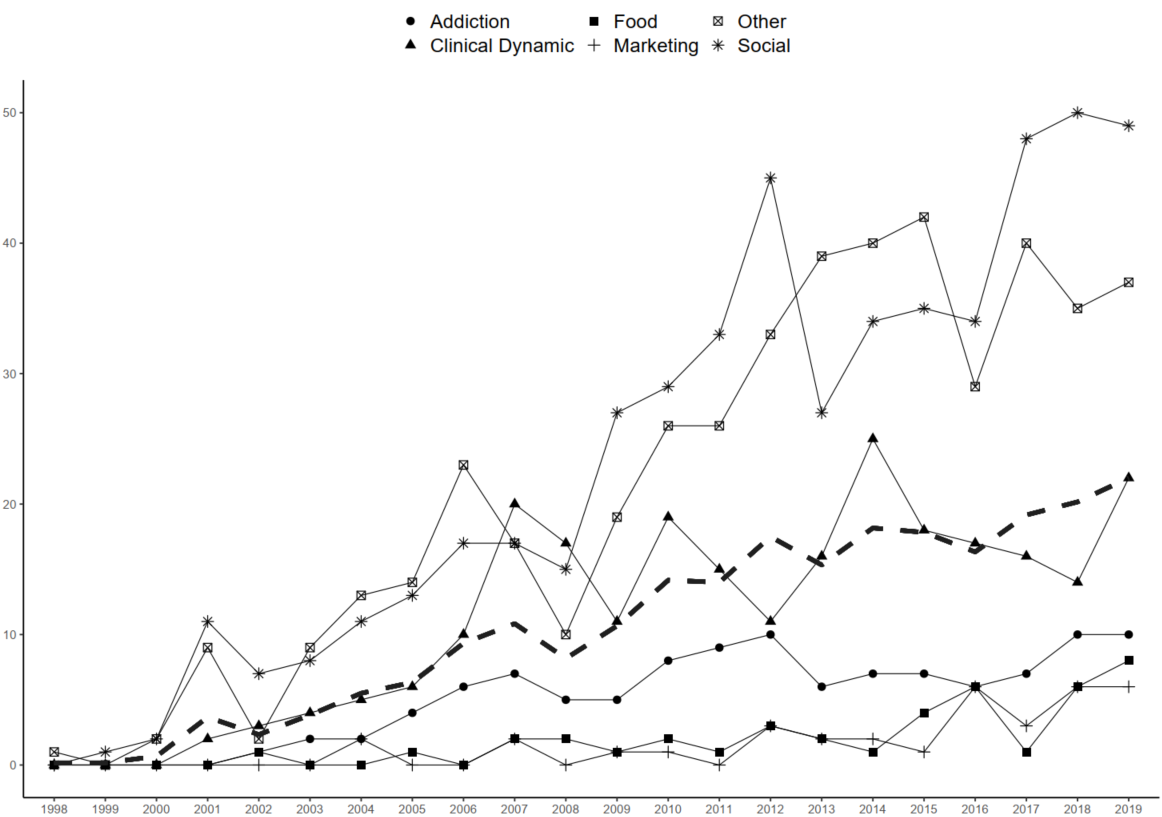
\includegraphics[width=0.8\linewidth]{yeartopic.png}
	\caption{\label{fig:topicyear} Trend lines of each field of application of the IAT throughout from 1998 to 2019. }
\end{figure}

The dashed line in Figure (\ref{fig:topicyear}) represents the average trend of the IAT use across different fields of applications, and it clearly point a constant an on-going growth in the IAT use throughout the years. 

Trend lines for the fields of application Social psychology and Other appear always above the mean trend line. Clinical and dynamic psychology trend line is the most inconsistent one throughout the years. Specifically, it shows a steady growth until 2007-2008, with a drop in 2009, followed by a vacillating trend until 2015, where it encounters a sort of \emph{plateau} with a final peak in 2019. The trend lines of fields pf applications Food and Marketing are similar between each other, both pointing at a higher use of the IAT during the past few years. 

Besides the general fields of applications of the IAT, it is interesting to delve deeper on the specific topics for which the IAT was employed.  

Figure \ref{fig:wordcloud} Reports the most common topics for which the IAT has been used throughout the years. 

\begin{figure}
	\centering
	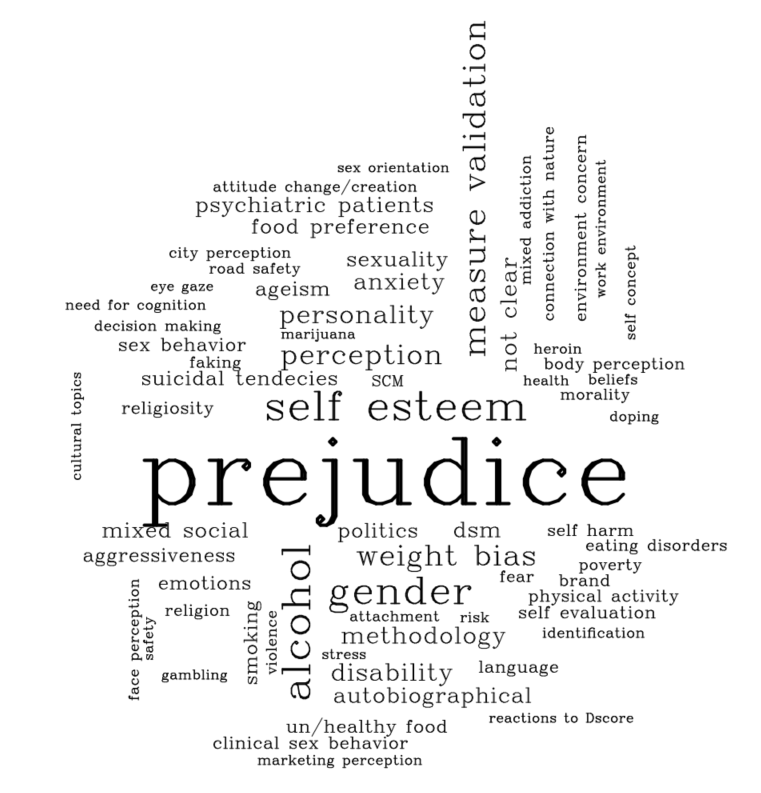
\includegraphics[width=0.5\linewidth]{wordcloudtopic.png}
	\caption{\label{fig:wordcloud} IAT fields of application word cloud.  The bigger the word font, the more common the use of the IAT for the investigation of that specific topic.}
\end{figure}

It is not surprising to note that the most common use of the IAT was for the investigation of implicit stereotypes and attitudes, such as implicit racial prejudice, gender stereotypes, attitudes towards obese people and other social groups, such as psychiatric patients and people with disabilities. Indeed, the IAT was specifically designed for tapping the automatic aspects of attitudes, making it more resistant to self-presentation biases \cite<e.g.,>{greenwald2009}. As such, its use is particularly appealing for the investigation of socially sensitive topics. 

Other interesting application of the IAT concerns the investigation of addiction towards different drugs or unhealthy behaviors, such as alcohol consumption or smoking, personality traits, and self-perception. 

In the following paragraphs, a brief summary of the IAT applications in each of the above-mentioned fields is provided. 

\paragraph{IAT in Social psychology.} Given the IAT resistance to self-presentation strategies and hence to responses altered by social desirability \cite<e.g.,>{greenwald2009}, its use is particularly popular for the investigation of socially sensitive topics. Most of the studies employing the IAT in Social psychology deals with the investigation of out-group stereotypes and prejudice, specifically related to racial prejudice. Studies on this topic are followed by studies focused on gender stereotypes, and on the investigation of illness-related attitudes. Illness-related attitudes indicate attitudes towards people with either mental or physical disabilities, psychiatric patients, people with HIV, cancer patients and day-care patients in general, and suicide survivals.

Despite with lower frequency, IAT is also used to assess attitudes towards people professing different religions, towards non-native English speakers, and bias towards people with low incomes. Papers composed by multi studies in which attitudes towards multiple out-groups (e.g., out-group prejudice and weight bias) were concurrently investigated were common. The IAT was also used to investigate topics related to the Stereotype Content Model  \cite<SCM;>{fiske2002}, including infra-humanization, and to investigate the effectiveness of experimental manipulation to change/induce attitudes, even towards non-real groups.

It is interesting to note the specific samples on which studies using the IAT have been carried out. Specifically, the IAT appears to be widely used among samples composed of hospital personnel (i.e., doctors, nurses, therapists), adults, undergraduates, and work personnel (i.e., CEOs, hiring personnel, university boards). 

The common goal of the studies investigating out-group prejudice and stereotypes, illness related attitudes, and weight bias among hospital personnel was to understand whether the implicit bias towards the specific out-group influenced the quality of the provided care on the probability of suggesting a specific surgery. The IAT was applied in a similar vein on samples composed of work personnel. Specifically, these studies were aimed at understanding whether implicit biases could undermine the probability of people belonging to minority groups, such as African-American people in the US, to be hired in a corporation or to win a position in Academia. Another interesting IAT application was for the investigation of the implicit out-group prejudice or implicit gender stereotypes of teachers. The aim of these studies was to understand whether teachers’ gender implicit attitudes (e.g., implicitly associating males with math and females with humanistic subjects) or their racial implicit attitudes (e.g., associating European-American children with higher intelligence than Hispanic children) could influence their behaviors towards their pupils.

\paragraph{IAT in Clinical and dynamic psychology.} Concerning Clinical and dynamic psychology, the IAT was mostly used for the implicit assessment of self-esteem. Personality traits (e.g., Big Five personality traits), anxiety, and DSM psychological disorders (both personality and mood disorders) were fairly investigated as well. The IAT was also commonly used for the implicit assessment of suicidal tendencies, aggressiveness, emotions, and clinical sex behavior (e.g., pedophilia). 

\paragraph{IAT in Addiction research.} Vast majority of studies using the IAT in research on addiction were focused on the investigation of alcohol addiction, followed by studies on nicotine and smoking addiction. The concurrent investigation of multiple addictions, such as drinking and smoking or drinking and gambling, was quite uncommon. The IAT was used for investigating cocaine addiction in just one study. 
These studies are mostly carried out on clinical samples of people with a diagnosis of addiction to some substance, but also studies carried out on college students are fairly common. 

\paragraph{IAT in Food research.} The most common aim with which the IAT is used in Food research was to investigate the preference for different kind of food, the preference for healthy over unhealthy food, or food perception. IAT was also employed for investigating attitudes towards dieting. Less common topic were food craving, food self--control, and the effect of the time of day on food preference. 

\paragraph{The IAT in marketing research.} Marketing research is one of the most recent field of applications of the IAT. Most of the studies are focused on the implicit evaluation of the preference for a brand over another. Additionally, the IAT has been employed for studying the processes driving the decision to purchase some products, and the role of products labels and packaging in influencing the purchase of that specific product.

\paragraph{The IAT in macro-area Other.} Studies included in this field of application include cover a broad and extensive range of topics, from gender perception of odds and even numbers \cite{gendernumber} to work related stress \cite{workstress} and romantic attachment \cite{romantic}.
Studies aimed at the validation of the IAT are included as well, and they compose the vast majority of the studies in this field of applications. They are followed by studies on human perception and studies on methodology. The distinction between measure validation papers and methodology papers is quite subtle. Measure validation studies include papers aimed at the validation of the IAT procedure \cite<e.g.,>{Greenwald1998}, its score \cite<e.g.,>{Greenwald2003}, and the factors that may affect the IAT effect \cite<e.g.,>{bluemke2006}. Methodology includes studies in which existing formal models were used for modeling IAT data, such as the application of the Many-Facet Rasch Measurement Model \cite{linacre1989} in \citeA{anselmi2011} or the application of the Diffusion Model \cite{ratcliff1978} in \citeA{Klauer2007}. Studies aimed at the validation of \emph{ad-hoc} models for IAT data, such as the Quad Model \cite{Conrey2005} or the Discrimination-Association Model \cite{stefanutti2013} are included under the label methodology as well.

\section{The Single-Category Implicit Association Test}\label{sec:sciat}

The IAT has vastly proven its effectiveness and usefulness in providing a relative measure of the preference towards one object category compared with the contrasted one. Many attitudes or preference objects present a clear contrasted category, so that it is meaningful and useful to investigate the relative preference/attitudes \cite{greenwald2000}. Sticking with the Coke-Pepsi IAT example in Section \ref{sec:iat}, faster responses in the Coke/Good-Pepsi/Bad associative condition might be due to either a preference for Coke (faster responses in sorting \emph{Coke} images and \emph{Good} attributes with the same response key), a dislike for Pepsi (faster responses in sorting \emph{Pepsi} images and \emph{Bad} attributes with the same response key), or even a combination of the two. The resulting IAT effect is not able to actually acknowledge for the specific preference/dislike driving the responses. One could try to decompose the IAT effect by computing separate scores for the trials in which \emph{Good} attributes and \emph{Coke} images are associated and in which \emph{Bad} attributes and \emph{Coke} images are associated. Even by doing so, it is not possible to obtain an absolute measure of the preference towards one of the two beverages \cite{nosek2005}. The IAT is based on a comparative task and, as such, it can only result in a comparative measure.

Clearly, when the focus of the research is on the assessment of the absolute positive or negative evaluation of a single object, the IAT might not represent the best choice. Consider the case of self-esteem evaluation. In this case, the interest would be on how much a person values himself/herself. However, studies that employed the IAT for implicitly investigating this construct contrasted the category \emph{Self} or \emph{Me} with a generic category, like \emph{Other} \cite<e.g.;>{selfesteemOther} or \emph{Not Me} \cite<e.g.,>{selfesteemME}. Consequently, the measure resulted in an indirect evaluation of how much a person valued himself/herself in comparison to others, and not in how much a person valued himself/herself \cite{karpinski2006}. 

Moreover, since the final effect would depend on the relative evaluation between the two categories, the choice of the contrasted category is of the uttermost importance. In some cases, a clear contrasted category is not available, and the researcher has to make arbitrary choices. Consider the Coke-Pepsi IAT example again. The positive or negative evaluation of Coke is strongly dependent on the positive or negative evaluation of Pepsi. By changing the contrasted category, for example from Pepsi to Dr. Pepper, the evaluation of Coke might also change since this evaluation is relative to the alleged opposite of Coke.

Different alternative measures have been introduced to overcome the issue of the relativeness of the implicit measure, like the Single Category Implicit Association Test \cite<SC-IAT;>{karpinski2006}, which results from a slight modification of the IAT procedure. As the IAT, the SC-IAT measures the strength of associations between concepts by considering the speed and accuracy with which different stimuli are sorted in their reference category. The assumption that underlies the functioning of the SC-IAT is the same as that underlying the IAT functioning, namely, that it is easier to sort together exemplars of two categories when they are strongly associated with each other than when they are not. However, differently from the IAT, the exemplars of only one object category (e.g., \emph{Coke} in a Coke SC-IAT), along with the exemplars of two attributes categories, are presented. The usual structure of a Coke SC-IAT is illustrated in Table \ref{tab:sciatstructure}. 

\begin{table}[h!]
	\centering \doublespacing
	\caption{Coke SC-IAT structure \protect\cite<Adapted from >{karpinski2006}.}
	\label{tab:sciatstructure}
	\begin{tabular}{p{1cm} p{1.4cm} p{4cm} p{4cm} p{4cm}}
		\toprule
		Block & Trials & Function  & Left Response key & Right Response key \\
		\midrule
		B1 & 24 & Associative practice & Good \& Coke & Bad \\
		B2 & 72 & Associative Test & Good \& Coke & Bad \\
		B3 & 24 & Associative practice & Good  & Bad \& Coke \\
		B4 & 72 & Associative Test & Good  & Bad \& Coke \\
		\bottomrule
		\multicolumn{5}{p{13cm}}{\onehalfspacing\emph{Note:} The order of presentation of Blocks B1 and B2 and B3 and B4 are counterbalanced across respondents.}
	\end{tabular}
\end{table}

The SC-IAT is usually composed of 4 blocks, two of which (Blocks B1 and B3) are associative practice blocks used to let the respondents familiarize with both the stimuli and the task. 
In the first critical block, that is, the first critical condition, the target object \emph{Coke} and \emph{Good} attributes share the same response key, while \emph{Bad} attributes are sorted with the opposite response key (Coke/Good-Bad condition). In the contrasting associative condition, target object \emph{Coke} is sorted with the same response key as \emph{Bad}, while \emph{Good} words are sorted with the opposite response key (Coke/Bad-Good condition).  
The SC-IAT administration procedure usually includes a response time window (rtw) at 1,500 ms, after which the stimulus disappears and a warning message (e.g., ``Respond more quickly!'') is given to the respondent. Moreover, every correct response is signaled by a green ``O'', while every incorrect response is signaled by a red ``X''. Differently from the IAT, respondents do not have to correct their incorrect responses to go on with the experiment. The presence of the rtw and the feedback for every response are the two characteristics that differentiate the SC-IAT from the Single Target Implicit Association Test \cite<ST-IAT;>{stiat}. Nonetheless, the names (and procedures) of the two measures are used interchangeably \cite<e.g.,>{bar2014}.
The SC-IAT effect results from the difference in respondents' performance between the two contrasting conditions, and it is usually expressed by a modification of the \emph{D-score} \cite[see Chapter \ref{sec:sciatD}]{karpinski2006}.



\section[Fully-crossed design]{Implicit measures fully-crossed design}\label{sec:cross}

In tasks like the IAT and the SC-IAT, stimuli representing each of the reference categories are presented multiple times, both within and between the associative conditions. Each stimulus exemplar is also presented multiple times to each respondent, both within and between the associative conditions. Thus stimuli and respondents are crossed with each other (multiple responses to the same stimulus by the same participant), and they are in turn crossed with the associative conditions (multiple responses on the same stimulus by the same respondents both within and between the conditions). Besides being the design characterizing both the IAT and the SC-IAT, this type of design (i.e, fully-crossed design) is rather common in experimental psychology, from linguistic to social cognition \cite{Westfall2014}. Data deriving from this design should be carefully analyzed to account for the sources of dependencies that might end into misleading results and undermine their replicability.  

The multiple observations on the same respondents and on the same stimulus generate a random noise at the level of the single observation that cannot be ignored to obtain reliable parameters estimates. The fully-crossed structure results in a unique combination respondent $\times$ stimulus for every repetition of the stimuli in each associative condition. Consequently, different sources of variability and dependency -- related to participants, stimuli, conditions, and to their interaction -- have to be expected \cite{Barr2013, Westfall2014, wols2017}. 

Suppose that two respondents, Ben and Angela, are administered with the Coke-Pepsi IAT (or the Coke SC-IAT) presented in Section \ref{sec:iat} (or Section \ref{sec:sciat}). Ben might be, on average, more accurate (or faster) than Angela, and this may be due to different reasons pertaining Ben's and Angela's characteristics. This between--response variability can be considered as the expression of the variability due to respondents' individual differences, across the associative conditions. 

The exemplars used for representing the categories are important as well. Consider the \emph{Coke} category. The logo of the company can be immediately recognized as belonging to the \emph{Coke} category, hence having a higher probability of being immediately (and accurately sorted)  into the correct category. Conversely, an old-fashioned image of a can of Coke might be less familiar and could hence require more time for being recognized and accurately sorted in the correct category. The difference caused by the properties of the stimuli generates a variability at the stimuli level (i.e., between stimuli variability), which can be considered as the expression of the variability due to the stimuli characteristics eliciting different responses, across the associative conditions. 

Ben and Angela's performance might be impaired or facilitated by the associative conditions. For instance, the difference between their performance might be reduced in the condition in which Coke is associated with positive attributes and Pepsi is associated with negative attributes. In this case, Angela might be facilitated because she is particularly fond of Coke and it is easier for her to associate Coke exemplars with positive attributes, while Ben is already a good respondent. In the opposite condition, the difference in their accuracy or speed performance might be exacerbated. Angela, who is already a low accuracy respondents, might find particularly difficult to associate Coke with negative words. This variability (i.e., the within--respondents between conditions variability) can be considered as the effect of the IAT associative conditions on the respondents' performance. It expresses the deviation of each participant from the estimate of the average performance in each condition. 

Also the categorization of the stimuli can benefit from the associative condition in which they are presented. For instance, the Coke exemplars might receive more accurate and faster responses when they share the response key with positive attributes than when they share it with the negative response key. This within--stimuli between--conditions variability can account for this intra-stimulus variability, and can hence be interpreted as the expression of how the IAT associative condition is affecting the stimuli categorization. 

%These are the main sources of variability that can be found in IAT or SC-IAT data and that have to be accounted for in order to obtain reliable estimates. 
%However, there is a part of variability that is due to the reactions of each respondent to each stimulus 
%Nonetheless, there's still a part of variability that is left out, which is the variability due to the presentation of each stimulus to each participant, or, in other words, the reaction of each respondent to each stimulus. 

When these sources of variability are not included into a statistical model able to account for them, they can influence the estimation of any parameters, or the computation of any scores. 
Thus, ignoring the sources of variability and the dependency between the IAT or the SC-IAT observations may result in biased parameter estimates (such as incorrect standard errors), which may lead to an overestimation (or underestimation) of the importance of experimental effects \cite{judd2017, mc1989}. Moreover, by overlooking the sampling variation related to the stimuli, the information that can be gathered from them is completely neglected \cite{wols2017}. 

\subsection{More than one implicit measure}
It is not uncommon that the IAT and the SC-IAT are used concurrently to obtain both a comparative measure between the two objects of interest and an absolute evaluation towards each of them \cite<e.g.,>{bulmer2018implicit, glashouwer2013low}. When both the implicit measures are used, their data are analyzed separately, and their effects are usually expressed by separate \emph{D-score}s. The \emph{D-score}s are effect size measures obtained by standardizing the difference in the average response times between the two contrasting conditions. These indexes are easy to compute and can provide a quick and interpretable measure of the implicit constructs under investigation. Nonetheless, they come with issues that cannot be ignored, both when the IAT and the SC-IAT are used as single measures and when they are concurrently employed.

Beyond the issues related to the computation of scores like the \emph{D-score} on data structure such as those of the IAT and the SC-IAT, there are also issues arising from the concurrent use of the implicit measures. When the IAT and the SC-IAT are used together and separate \emph{D-score}s are computed, the within--respondents between--measures variability is completely ignored, as well as method specific variance. Any possible carry-over effects or dependency due to the multiple observations on the same respondent, both within and between measures and their respective associative conditions, are not accounted for. Furthermore, since the same stimuli are usually employed across the IAT and the SC-IAT, other sources of dependency at the stimuli level have to be expected. Consequently, the resulting \emph{D-score}s are including a proportion of unwanted error variance directly related to the sources of dependency at different levels.   

\chapter{Classic scoring of implicit measures}\label{classicscore}
This chapter deals with the classic scoring measures for the IAT and the SC-IAT. Firstly, the scoring algorithms for both the IAT and the SC-IAT are illustrated and described. Then, new algorithms for the scoring of both implicit measures are presented, and the predictive ability in respect of a behavioral choice of both the classic and the newly developed algorithms is investigated and compared in an empirical study. 
Finally, the development of new tools for easily computing the IAT and SC-IAT scores is presented.

\newpage
\section{IAT D-score}\label{sec:iatD}
\citeA{Greenwald2003} introduced different variations of the \emph{D-score} algorithm, illustrated in Table \ref{tab:Doverview}. These variations result from the combination of error correction strategies (``Error replacement'' in Table \ref{tab:Doverview}) and treatment for fast responses (``Lower tail treatment'' in Table \ref{tab:Doverview}).
\begin{table}[th!]
	\centering \doublespacing
	\caption{\label{tab:Doverview} Overview of \emph{D-score} algorithms. }
	\begin{tabular}{p{2cm}p{7cm}p{7cm}}
		\toprule
		Algorithm & Error replacement & Lower tail treatment\\\hline
		\emph{D}1 & Built-in correction & No \\
		\emph{D}2 & Built-in correction & Delete trials $<$ 400 ms \\
		\emph{D}3 & Mean $+$ 2\emph{sd} & No\\
		\emph{D}4 & Mean $+$ 600 ms & No \\
		\emph{D}5 & Mean $+$ 2\emph{sd} & Delete trials $<$ 400 ms\\
		\emph{D}6 & Mean $+$ 600 ms & Delete trials $<$ 400 ms \\
		\bottomrule
		\multicolumn{3}{p{16cm}}{\onehalfspacing\emph{Note:} For all algorithms, trials with latency $>$ 10,000 ms are discarded. For the algorithm in which error responses are replaced with the average response time plus a penalty, the average response time is computed on correct responses only.}
		\end{tabular}
	\end{table}

Blocks B1, B2, and B5 in Table \ref{tab:iatstructure} are considered as pure practice blocks and are hence discarded from the computation. Only trials from Blocks B3, B4 and B6, B7 are used for the computation.  

The error correction strategies based on the built-in correction (\emph{D1} and \emph{D2}) refer to the IAT administration including feedback, as described in Section \ref{sec:iat}, for which error respondents have to correct their error responses. The response time considered for the computation of the \emph{D-score} is the response time at the first (incorrect) response increased by the time required to correct it. All other algorithms (from \emph{D1} to \emph{D6} in Table \ref{tab:Doverview}) use a \emph{post-hoc} error correction strategy, for which error responses are replaced by the average response time of the correct responses in the block in which the error occurred increased by a standard penalty (i.e., either 600 ms or twice the standard deviation).
The other feature differentiating the \emph{D-score} algorithms is the lower tail treatment, according to which fast trials ($< 400$ ms) are discarded or not.

Regardless of the specific guidelines for each algorithm, the core procedure for computing the \emph{D-score} is the same. Firstly, the \emph{D-score}s for the associative practice blocks (Eq. \ref{eq:practice}) and for the associative test blocks (Eq. \ref{eq:test}) are computed: 
%
\begin{equation}\label{eq:practice}
	D_{\text{practice}} = \frac{M_{\text{B6}} - M_{\text{B3}}}{\text{\emph{SD}}_{\text{B6, B3}}}, 
\end{equation}
%
and 
%
\begin{equation}\label{eq:test}
D_{\text{test}} = \frac{M_{\text{B6}} - M_{\text{B3}}}{\text{\emph{SD}}_{\text{B6, B3}}}.
\end{equation}

In both cases, the difference in the average response time between the two critical blocks is divided by the standard deviation computed on the pooled trials of both blocks. Once $D_{\text{practice}}$ and $D_{\text{test}}$ are obtained, it is possible to compute the actual \emph{D-score}: 
%
\begin{equation}\label{eq:dscore}
	\text{\emph{D-score}} = \frac{D_{\text{practice}} + D_{\text{test}}}{2}.
\end{equation}

The block orders in Equation \ref{eq:practice} and Equation \ref{eq:test} is arbitrary and can be reversed. The resulting \emph{D-score} has to be interpreted accordingly. Sticking with the Coke-Pepsi IAT structure depicted in Table \ref{tab:iatstructure}, if the \emph{D-score} is computed following the order of the blocks in Equation \ref{eq:practice} (i.e., $M_{\text{B6}} - M_{\text{B3}}$) and in Equation \ref{eq:test} (i.e.,$M_{\text{B7}} - M_{\text{B4}}$), a positive score would indicate slower responses in Pepsi/Good-Coke/Bad condition than in Coke/Good-Pepsi/Bad one, probably indicating a preference for Coke over Pepsi. Vice versa, if the order of the Block in Equations \ref{eq:practice} and \ref{eq:test} is reversed (i.e., $M_{\text{B3}} - M_{\text{B6}}$ and $M_{\text{B4}} - M_{\text{B7}}$, respectively), a positive score would indicate slower responses in the Coke/Good-Pepsi/Bad condition than in the Pepsi/Good-Coke/Bad condition, indicating a possible preference for Pepsi over Coke.
			 

\section{SC-IAT D-score}\label{sec:sciatD}

Since blocks B1 and B3 (Table \ref{tab:sciatstructure}) are considered as pure practice blocks, they are not considered for the computation of the SC-IAT \emph{D-score}. If a rtw was included in the administration procedure, all responses exceeding it are considered as non responses and are hence discarded from the computation. All responses with a latency faster than 350 ms are discarded, and error responses are replaced with the average response time of the block in which the error occurred inflated by a standard penalty of 400 ms. 

After cleaning and preparing the data, the SC-IAT \emph{D-score} is simply computed as the difference in the average response time of the two critical blocks (i.e., $M_{\text{B4}} - M_{\text{B2}}$) divided by the standard deviation computed of the correct trials of both blocks. As for the IAT, the order of the critical blocks is arbitrary and the interpretation of the \emph{D-score} depend on that order. 

Consider the Coke SC-IAT in Table \ref{tab:sciatstructure}. If the \emph{D-score} is computed as the difference between Block B4 and Block B2, a positive score would indicate slower responses in the Bad/Coke condition than in the Good/Coke one, standing for a positive evaluation of Coke. Vice versa, if the score is computed in the opposite direction (i.e., $M_{\text{B2}} - M_{\text{B4}}$), a positive score would indicate slower responses in the Good/Coke condition than in the Bad/Coke condition, indicating a plausible negative evaluation of Coke. 


\section[A fairer comparison]{A fairer comparison between the IAT and the SC-IAT}

The aim of this study was to provide a fairer comparison of the predictive ability of the IAT and the SC-IAT in respect to a behavioral choice. 

In Study 1, \cite{karpinski2006} directly investigated and compared the predictive ability of a Soda IAT, that of a Coke SC-IAT, and that of a Pepsi SC-IAT, in respect to a soda, namely Coke vs Pepsi. As their results were suggesting, measures obtained from both the Soda IAT and the Pepsi SC-IAT played  a role in predicting the actual soda choice, while the measure obtained from the Coke Sc-IAT did not contribute to the choice prediction. 
%\citeA[Study 1]{karpinski2006} provided a direct comparison between the IAT and the SC-IAT. These authors investigated the capacity of a Coke-Pepsi IAT, a Coke SC-IAT and a Pepsi SC-IAT of predicting the soda choice between Coke and Pepsi. Results showed that both the Coke-Pepsi IAT and the Pepsi SC-IAT allowed for predicting the soda choice, while the Coke SC-IAT was unrelated to the choice. 
Drawing on this results, authors speculated that the soda choice is more guided by a positive evaluation of Pepsi than by a negative evaluation of Coke. Nonetheless, the direct comparison between the predictive ability of the two implicit measures has been poorly investigated. 
Despite the study by \cite{karpinski2006} provided interesting information on the functioning of implicit processes and the comparison between implicit measures, it also showed some shortcomings that might have undermined the validity of their results. Firstly, the sample size was rather small, and results should hence be interpreted with caution. Moreover, the comparison between the predictive ability of the implicit measures might have been affect by issues concerning both their administration and scoring procedures. The IAT and the SC-IAT differed in both the number of trials and the number of exemplars representing each category. The SC-IAT employed more stimuli than the IAT, for both the evaluative dimensions (twenty-one exemplars for each SC-IAT evaluative dimension versus five exemplars for each IAT evaluative dimension), and the object categories (seven exemplars for each SC-IAT target object category and five exemplars for each IAT target object category). Furthermore, the administration of the SC-IAT included a rtw (i.e., the stimulus was disappearing from the screen after 1,500 ms). Conversely, the IAT did not have such a constraint on the responses. Beyond making the task more difficult, the presence of a rtw produces a sense of urgency that it is otherwise missing \cite{karpinski2006}. Consistently with the SC-IAT administration procedure presented in Section \ref{sec:sciat}, respondents were given feedback for each correct and incorrect response. No feedback, either for correct or incorrect responses, was given in the IAT. The procedures differed also on the labels used for representing the positive and negative evaluative dimensions (\emph{Pleasant} vs \emph{Unpleasant} for the IAT and \emph{Good} vs \emph{Bad} for the SC-IAT). Also the response keys used for sorting the stimuli hanged across measures.  The IAT \emph{D-score}s were computed according to the \emph{D-score} procedure in \citeA{Greenwald2003}, despite \citeA{karpinski2006} fails to report the exact algorithm they have employed. The SC-IAT \emph{D-score} presented in Section \ref{sec:sciatD} was used for computing the SC-IAT \emph{D-score}.

%To the best of our knowledge, only \citeA{karpinski2006} provided a systematic comparison between the predictive ability of the two implicit measures. However, their study presented some drawbacks that might have undermined the validity of their results. Firstly, the sample size was rather small, and results should hence be interpreted with caution. Moreover, the comparison between the predictive ability of the two implicit measures might have been affect by issues concerning bothe their administration and scoring procedures. The IAT and the SC-IAT differed in both the number of trials and the number of stimuli used for representing each category. The SC-IAT employed more stimuli than the IAT, for both the evaluative dimensions (twenty-one stimuli for each SC-IAT evaluative dimension versus five stimuli for each IAT evaluative dimension), and the object stimuli (seven stimuli for each SC-IAT target object category and five stimuli for each IAT target object category). Furthermore, the administration of the SC-IAT included a response time window (RTW), for which after 1,500 ms the stimulus on the screen disappeared. Conversely, the IAT did not have such a constraint on the responses. Beyond making the task more difficult, the presence of a RTW induce a sense of urgency of giving the response which is missing when the RTW is not included \cite{karpinski2006}. According to SC-IAT administration procedure presented in Section \ref{sec:sciat}, respondents were given feedback for each correct and incorrect response,while this was not done in the IAT case. The procedures differed also on the labels used for representing the positive and negative attribute categories (\emph{Pleasant} and \emph{Unpleasant} for the IAT and \emph{Good} and \emph{Bad} for the SC-IAT), and on the response keys used for sorting the stimuli.  The IAT \emph{D-score}s were computed according to the \emph{D-score} procedure in \citeA{Greenwald2003}, despite \citeA{karpinski2006} fails to report the exact algorithm they have employed. The SC-IAT \emph{D-score} presented in Section \ref{sec:sciatD} was used for computing the SC-IAT \emph{D-score}.

Given the differences between administration and scoring, the comparison between the ability of the IAT and that of the SC-IAT to predict a behavioral outcome might have been unfair. To the best of our knowledge, there is neither a scoring procedure employing the same criteria for both the IAT and the SC-IAT, nor an attempt to align the two implicit procedures to allow for a fairer comparison between their predictive capacity. It would be interesting to compare the predictive ability of the two implicit measures by using the same scoring procedure and by keeping the administration as similar as possible, while acknowledging their key features (e.g., block types and usual length of the blocks). If by using the same scoring method and by reducing the differences related to the administration procedures there are still differences in the predictive ability of the two measures, these differences can be reasonably attributed to the implicit procedure itself.

To obtain a fairer comparison between the two implicit measures, both administration (e.g., stimuli, response time window, feedback) and scoring of the two procedures have been aligned.

\subsection{Method}

To test the predictive ability of the new scoring procedures, one Chocolate IAT, one Milk chocolate SC-IAT, and one Dark chocolate SC-IAT were developed. 
The decision to use Chocolate as the object category was driven by different reasons. Firstly, chocolate preference should not be sensitive to social desirability, and hence respondents would have no concerns in reporting their actual chocolate preference. Moreover, it offers the chance to ask for a behavioral choice disguised as a reward for the participation.

Inquisit \cite<3.0;>{inquisit3} was used for administering both implicit measures (i.e., IAT and the two SC-IATs) and the demographic questionnaire.

\paragraph{Participants.}

Participants were recruited at the University of Padova. One-hundred and sixty-one people (F $= 63.55$\%, Age $= 23.95 \pm 2.83$) volunteered to take part in the study, with no compensation. Participants were informed about the confidentiality of the data, and the possibility of withdrawing from the experiment at any time they wished. They were asked for their consent to take part in the study. Majority of the participants were students ($94.08$\%), including both undergraduates, master, and PhD students. Only two participants reported to have a PhD title, while the majority reported to have a bachelor’s degree (43.42\%), immediately followed by those who reported having a high school diploma (32.24\%) and a master’s degree (23.03\%). 

\paragraph{Materials and Procedure.}

Chocolate stimuli were composed by seven images of chocolate that were modified to represent either Dark or Milk chocolate. Seven images for each type of chocolate were used. Three independent judges evaluated the stimuli regarding their properties, specifically whether they were clearly identifiable as Dark or Milk chocolate images. The three judges agreed on the representativeness of the stimulus of the category to which it was supposed to belong. All chocolate images were presented on a white background. 
%The stimuli and the Inquisit script for running the experiment can be retrieved in an online repository (\url{https://osf.io/cnq4u/}). 
In the Chocolate IAT, both Dark and milk chocolate images were used. In the two SC-IATs, only either Dark (Dark SC-IAT) or Milk (Milk SC-IAT) chocolate images were used. In all implicit procedures, evaluative attributes categories were composed by 13 stimuli each. The evaluative categories were labeled as \emph{Positive} (i.e., ``good'', ``laughter'', ``pleasure'', ``glory'', ``peace'', ``happiness'', ``joy'', ``love'', ``wonderful'', ``beautiful'', ``excellent'', ``heaven'', ``marvelous'') or \emph{Negative} (i.e., ``evil'', ``bad'', ``horrible'', ``terrible'', ``annoying'', ``pain'', ``failure'', ``hate'', ``nasty'', ``disaster'', ``agony'', ``ugly'', ``disgust''). Object categories were labeled as \emph{Dark} or \emph{Milk}. Response key ``E'' was used for sorting the stimuli belonging to the categories represented on the left-side of the screen. Response key ``I'' was used for sorting the stimuli belonging to the categories represented on right side of the screen. Differently for the SC-IAT procedure described in Section \ref{sec:sciat}, SC-IAT practice Blocks B1 and B3 were composed of 20 trials, as for the practice blocks of the IAT. Neither the IAT nor the SC-IATs included a built-in correction or a response time window. Respondents did not receive any feedback on their performance, and they were asked to be as fast and accurate as they could in performing the tasks. 

Additionally, respondents were explicitly asked to report their evaluation for Dark and Milk chocolate on two distinct items (``How much do you like Dark/Milk chocolate?'') rated from ``0 – Not at all'' to ``5 – Very much''. The order of presentation of the implicit measures was counterbalanced across participants, and the explicit assessment was kept constant after the administration of implicit measures. 

As a reward for their participation, respondents were offered with a free piece of Dark or Milk chocolate. The experimenter registered respondents' choices after they left the laboratory.

\emph{Chocolate IAT:} The critical blocks were composed of 60 trials each (20 practice and 40 test), defining the Dark-Good/Milk-Bad condition (DGMB), and the Milk-Good/Dark-Bad condition (MGDB). 

\emph{Dark SC-IAT:} The critical blocks were composed of 72 trials each, defining the Dark-Good/Bad (DG) and the Good/Dark-Bad (DB) conditions.

\emph{Milk SC-IAT:} As for the Dark chocolate SC-IAT, the critical blocks were composed of 72 trials each, defining the Milk-Good/Bad (MG) and the Good/Milk-Bad (MB) conditions.

\paragraph{Scoring.}

For the IAT, all \emph{D-score}s not including a built-in correction (algorithms \emph{D}3, \emph{D}4, \emph{D}5 and \emph{D}6 in Table~\ref{tab:Doverview}) were computed. The procedure described in Section \ref{sec:sciatD} was followed for computing the SC-IAT \emph{D-score}.
Since the SC-IAT administration did not include a rtw and there are no guidelines concerning the upper response times treatment, no deletion of upper time responses was applied. 

The scoring algorithms that have been introduced in this study result from different combinations of two main characteristics: The trials on which the standard deviation for the replacement of error responses was computed (i.e., only correct trials or all trials) and the quantity used for standardizing the difference in the response times between conditions (i.e., Cohen's pooled standard deviation or pooled trials standard deviation). 
The resulting eight combinations (identified by the letter ``\emph{m}'') are reported in Table~\ref{tab:modified}. 

\begin{table}[h!]
	\centering \doublespacing 
	\caption{\label{tab:modified} Overview of modified algorithms. for computing IAT and SC-IAT scores.}
	\begin{tabular}{l p{1cm} p{1cm}p{1cm} p{1cm}p{1cm} p{1cm}p{1cm} p{1cm}}
		\toprule
		Features & \emph{m}1 & \emph{m}2  & \emph{m}3 & \emph{m}4 & \emph{m}5 & \emph{m}6 & \emph{m}7 & \emph{m}8 \\
		\midrule
		Lower tail treatment & \multicolumn{8}{c}{$<$ 350 \emph{ms}}\\
		Upper tail treatment & \multicolumn{8}{c}{$>$ 10,000 \emph{ms}}\\
		Error treatment & \multicolumn{4}{c}{Mean (Correct) $+$ 2 \emph{sd} (Correct)}  & \multicolumn{4}{c}{Mean (Correct) $+$ 2 \emph{sd}}\\
		Denominator & \multicolumn{2}{c}{Pooled trials} & \multicolumn{2}{c}{Cohen} & \multicolumn{2}{c}{Pooled trials} & \multicolumn{2}{c}{Cohen}\\  
		Denominator trials & Correct & All  & Correct & All & Correct & All & Correct & All \\
		\bottomrule
	\end{tabular}
\end{table}

While the classical procedure for the SC-IAT includes a default lower tail treatment, the lower tail treatment for the IAT depends on the \emph{D-score} algorithm (see Table~\ref{tab:Doverview}). To have a comparable score, a common lower tail treatment for both procedures was set (i.e., responses with a latency less than 350 \emph{ms} were discarded). Since it is not uncommon to find SC-IATs with no rtw, a common upper tail treatment for response times was proposed for both implicit measures (i.e., responses over 10,000 ms were discarded). Concerning the SC-IAT upper tail treatment, it might be argued that the deletion of the responses higher than 1,500 \emph{ms} (i.e., the rtw cut-off) could be a more appropriate threshold for slow responses. Nonetheless, the presence of the rtw itself produce an urge to respond that is missing when the response time window is not included in the administration procedure \cite{karpinski2006}. 
Since the SC-IAT is known to be an easier task than the IAT \cite{karpinski2006}, the latency of the responses in the SC-IAT tend to be faster than the latency of the responses in the IAT. Therefore, assuming 600 ms as a reasonable time for correcting the error response might be a too strong assumption for the SC-IAT data. Conversely, the penalty used in the SC-IAT (400 ms) might be not enough for acknowledging the response time needed for correcting the error response in the IAT. For this reason, the error responses are replaced by the average response times in the block in which the error occurred inflated by two times the standard deviation of the block.  

The pooled trials standard deviation and Cohen’s pooled standard deviation were computed either considering only correct responses or all trials. In the former case, the variability due to incorrect responses is not accounted for, while it is addressed in the latter case.
Finally, the IAT modified procedures were computed as the difference between the two associative conditions, instead of as the mean of the standardized average response time differences between the practice and test blocks.

Both classic and modified scoring for the IAT were computed so that positive scores indicated faster responses in associating Milk chocolate with positive attributes and Dark chocolate with negative attributes, and hence a likely preference for milk chocolate and/or a dislike for dark chocolate. Conversely, negative scores indicated faster responses in associating Dark chocolate with positive attributes and Milk chocolate with negative attributes, indicating a probable preference for Dark chocolate and/or a dislike for Milk chocolate. 

For the SC-IATs, both the classic and modified procedures were computed so that positive scores indicated faster responses in associating the target chocolate with positive attributes than with negative attributes, hence indicating a likely positive evaluation of the target chocolate. Conversely, negative scores indicated faster responses when the target chocolate was associated with negative attributes, and hence a probable negative evaluation towards the target chocolate.

\subsection{Results}

Data from nine participants were discarded. Eight of them explicitly reported not understanding the tasks they were asked to perform in either the IAT or one of the SC-IATs, while one of them registered too many fast responses, specifically on the Dark chocolate SC-IAT (more than 30\% of responses with a latency lower than 350 ms). The final sample was composed of 152 participants (F $= 63.82$\%, Age $= 24.03 \pm 2.8$2). Milk chocolate was chosen by the $48.03$\% of the participants. 

The median for the explicit evaluation of Dark chocolate was 3 (first quartile = 2, third quartile = 5). The median for the explicit evaluation of Milk chocolate was 4 (first quartile = 3, third quartile = 4). No trials exceeding the threshold of 10,000 ms were found in the SC-IATs. Three trials exceeding the 10,000 ms threshold were found in the IAT, and they were eliminated. 
The lowest percentage of trials faster than both $400$ ms ($1.39$\%) and $350$ ms ($0.19$ \%) were found in the IAT. The two SC-IATs showed similar percentages of trials faster that $350$ ms ($1.00$ \% and $0.90$ \% in Milk SC-IAT and Dark SC-IAT, respectively), as well as of trials faster than $400$ ms ($4.40$\% and $4.32$\% in Dark SC-IAT and in Milk SC-IAT, respectively).
All the implicit measures had the same overall percentage of correct responses ($95$\%).
The two SC-IATs showed similar average response latency (Dark SC-IAT $= 679.45 \pm 328.72$ ms, Milk SC-IAT $= 675.90 \pm 322.31$ ms). IAT average response time was $862.03 \pm 496.50$ ms. Descriptive statistics for all implicit measures, along with their correlation with explicit measures, are reported in Table~\ref{tab:Faircorrclassic}. 

\begin{landscape}
	\begin{table}[h!]
		\caption{\label{tab:Faircorrclassic} Descriptive statistics of the scores and correlations with explicit chocolate evaluations.}
		\centering \onehalfspacing
		\resizebox{\linewidth}{!}{
			%\small
			\begin{tabular}{ll d{2.7} d{2.2} d{2.2} d{1.5} d{1.5} l d{2.7} d{2.2}d{2.2}d{1.5}d{1.5}}
				\toprule
				& Modified & \multicolumn{1}{l}{\emph{M (sd)}}& \multicolumn{1}{l}{\emph{Min}} & \multicolumn{1}{l}{\emph{Max}} &\multicolumn{1}{l}{\emph{r}\textsubscript{Milk}} & \multicolumn{1}{l}{\emph{r}\textsubscript{Dark}}  & Classic &\multicolumn{1}{l}{\emph{M (sd)}} & \multicolumn{1}{l}{\emph{Min}} & \multicolumn{1}{l}{\emph{Max}} & \multicolumn{1}{l}{\emph{r}\textsubscript{Milk}} & \multicolumn{1}{l}{\emph{r}\textsubscript{Dark}} \\ \midrule
				\multirow[t]{8}{*}{IAT}  &  \emph{m 1}   & 0.64\,(0.62) & -1.91 & 1.72 & 0.40\sym{***}&-0.36\sym{***} &  \emph{D3}   & 0.41\,(0.41)  & -1.29 & 1.25 & 0.42\sym{***} & -0.38\sym{***}\\
				&  \emph{m 2}   & 0.64\, (0.60) & -1.86 & 1.69 & 0.40\sym{***}&-0.37\sym{***} &  \emph{D4}   & 0.39\, (0.39)  & -1.26 & 1.27 & 0.41\sym{***} & -0.38\sym{***}\\
				&  \emph{m 3}   & 0.73\, (0.73) & -2.25 & 2.84 & 0.39\sym{***}&-0.34\sym{***} &  \emph{D5}   & 0.40\, (0.41)  & -1.29 & 1.29 & 0.42\sym{***} & -0.37\sym{***}\\
				&  \emph{m 4}   & 0.72\, (0.70) & -2.12 & 2.59 & 0.39\sym{***}&-0.35\sym{***} &  \emph{D6}   & 0.39\, (0.39) & -1.26 & 1.32 & 0.41\sym{***} & -0.37\sym{***}\\
				& \emph{m 5}   & 0.64\, (0.63) & -2.29 & 1.72 & 0.40\sym{***}&-0.35\sym{***} &                  &  &              &    &  & \\
				& \emph{m 6}   & 0.64\, (0.60) & -1.85 & 1.69 & 0.40\sym{***}&-0.36\sym{***} &                  &  &              &    &  & \\
				& \emph{m 7}   & 0.72\, (0.75) & -2.34 & 2.85 & 0.39\sym{***}&-0.34\sym{***} &                  &  &              &    &  & \\
				& \emph{m 8}   & 0.72\, (0.71) & -2.11 & 2.60 & 0.39\sym{***}&-0.35\sym{***} &                  &  &              &    &  & \\
				\multirow[t]{8}{*}{Dark SC-IAT}  &   \emph{m1}   & -0.06\, (0.35) & -0.98 & 1.07 & -0.22\sym{**}&0.18\sym{*} &  \emph{D-Dark}    & -0.05\,(0.31)  & -0.74 & 0.78 & -0.19\sym{*} & 0.17\sym{*}\\
				& \emph{m 2}   & -0.06\, (0.34) & -1.03 & 0.94 & -0.23\sym{**}&0.17\sym{*} &     &     &     &     &     &  \\
				& \emph{m 3}   & -0.06\, (0.36) & -1.01 & 1.07 & -0.22\sym{**}&0.17\sym{*} &     &     &     &     &     &  \\
				&  \emph{m 4}   & -0.06\, (0.35) & -1.05 & 0.94 & -0.22\sym{**}&0.17\sym{*} &     &     &     &     &     &  \\
				&  \emph{m 5}   & -0.06\, (0.36) & -1.00 & 1.13 & -0.20\sym{*}&0.16\sym{*} &     &     &     &     &     &  \\
				&  \emph{m 6}   & -0.06\, (0.35) & -0.95 & 0.99 & -0.20\sym{*}&0.16 &     &     &     &     &     &  \\
				&  \emph{m 7}   & -0.06\, (0.36) & -1.04 & 1.13 & -0.19\sym{*}&0.16 &     &     &     &     &     &  \\
				&  \emph{m 8}   & -0.06\, (0.35) & -0.97 & 1.00 & -0.20\sym{*}&0.16 &     &     &     &     &     &  \\
				\multirow[t]{8}{*}{Milk SC-IAT}  &   \emph{m 1}   & 0.16\,(0.39) & -1.92 & 1.22 & 0.17\sym{*}&0.04 &  \emph{D-Milk}    & 0.15\, (0.33)  & -0.93 & 1.21 & 0.13 & 0.06\\
				&   \emph{m 2}   & 0.16\, (0.39) & -1.93 & 1.13 & 0.17\sym{*}&0.04 &     &     &     &     &     &  \\
				&  \emph{m 3}   & 0.16\, (0.41) & -1.92 & 1.5 & 0.17\sym{*}&0.04 &     &     &     &     &     &  \\
				&   \emph{m 4}   & 0.16\, (0.40) & -1.94 & 1.38 & 0.17\sym{*}&0.04 &     &     &     &     &     &  \\
				&  \emph{m 5}   & 0.16\, (0.38) & -1.39 & 1.23 & 0.15&0.05 &     &     &     &     &     &  \\
				&  \emph{m 6}   & 0.16\, (0.37) & -1.40 & 1.14 & 0.15&0.05 &     &     &     &     &     &  \\
				&  \emph{m 7}   & 0.17\, (0.39) & -1.39 & 1.51 & 0.16\sym{*}&0.05 &     &     &     &     &     &  \\
				&   \emph{m 8}   & 0.16\, (0.39) & -1.40 & 1.39 & 0.16\sym{*}&0.05 &     &     &     &     &     &  \\
				\bottomrule
			\end{tabular}
		}
	\end{table}
\end{landscape}

Regardless of the algorithm used, SC-IAT scores tended to have smaller effect sizes than IAT classic scores.
IAT modified scores showed higher effect sizes than IAT classic scores, and this effect was particularly noticeable for the scores using Cohen's pooled standard deviation. Modified and classic SC-IAT scores were more consistent between each other. 

Explicit Dark chocolate evaluation negatively and moderately correlated with explicit Milk chocolate evaluation ($r = -.39$, $p < .001$). IAT and Dark SC-IAT classic scores significantly correlated with both explicit chocolate evaluations. Milk SC-IAT classic score correlated with neither Dark nor Milk explicit evaluation. IAT modified scores significantly and moderately correlated with the explicit evaluations of both Dark and Milk chocolate. Modified scores of both SC-IATs significantly correlated with Milk chocolate explicit evaluation. Only the first four modified scores of Dark SC-IAT significantly correlated with Dark chocolate explicit evaluation. Correlation between Dark explicit evaluation and Milk SC-IAT scores (both classic and modified) was near zero. 

To check the consistency between the scores, Pearson's correlations were computed between the classic and modified scores and the explicit chocolate evaluations.

Correlation coefficients between classic IAT \emph{D-score}s ranged between $.99$ and $1.00$ (all $p$s $< .001$). Correlations between classic IAT scores and Dark SC-IAT classic score were all $-.21$ (all $p$s $<.010$). No correlations were found between classic IAT \emph{D-score}s and classic Milk SC-IAT score (correlations ranged between $-.04$ and $-.03$, all $p$s $>.050$). Classic \emph{D-Dark} and \emph{D-Milk} positively correlated between each other ($r = .15$, $p > .050$), but the correlation was not significant. Correlations between IAT modified scores ranged between $.97$ and $.99$ (all $p$s $< .001$). Their correlations with modified \emph{D-Dark} ranged between $-.31$ and $-.28$ (all $p$s $<.001$). Modified \emph{D-Milk} and modified IAT \emph{D-score}s did not correlate between each other (correlation coefficients ranged between $-.01$ and $.01$, all $p$s $> .050$). Correlations between modified \emph{D-Dark} ranged between $.98$ and $1.00$ (all $p$s $<.001$). Correlations between modified \emph{D-Milk} ranged between $.99$ and $1.00$ (all $p$s $<.001$). Correlation between modified \emph{D-Milk} and \emph{D-Dark} showed the same direction as the correlation between classic SC-IAT scores, ranging between $.15$ and $.20$. Interestingly, the correlation between all modified \emph{D-Milk} and modified \emph{D-Dark} from 5 to 8 (i.e., the scores in which  error responses were replaced by the mean added with twice the standard deviation computed on all trials) showed slightly stronger and significant correlations, ranging from $.18$ and $.20$ (all $p$s $<.010$). 

\paragraph{Behavioral outcome.}

Both classic and modified scores were regressed on the behavioral chocolate choice, coded as 0 for Dark chocolate choice (DCC) and 1 for Milk chocolate choice (MCC). For the IAT, each score was regressed on the choice in a separate logistic regression. Since the choice is a dichotomous task in which Dark chocolate is contrasted with Milk chocolate, it is plausible that positive and negative attitudes towards both type of chocolates had played a role in determining the actual choice. The scores obtained from each of the SC-IATs convey a unique information regarding the positive or negative evaluation of only one type of chocolate, therefore lacking a part of information that might be crucial in determining the choice. It can also be argued that, since the two SC-IATs are two different experiments, it would not make sense to use the linear combination of their scores for predicting the actual choice. Grounding on these considerations, both single Dark SC-IAT and Milk SC-IAT scores, as well as their linear combinations, were used for predicting the choice.

Nagelkerke’s \emph{R}$^2$ \cite{nagel} and model accuracy of prediction \cite{faraway2006} were used as criteria for the investigation of the scores best accounting for the actual choice. Specifically, model general accuracy (i.e., ratio between the number of chocolate choices correctly identified by the model and the total number of choices), DCC accuracy (i.e., ratio between the number of DCCs correctly identified by the model and total number of observed DCCs), and MCC accuracy (i.e., ratio between the number of MCCs correctly identified by the model and total number of observed MCCs) were computed. Results of the logistic regressions for predicting the chocolate choice are reported in Table \ref{tab:Fairsingchoice}.

\begin{landscape}
%\begin{onehalfspacing}
		\small
	%\begin{table}
	%	\caption{\label{tab:singchoice} Choice prediction results, single predictors.}
	%\centering \doublespacing
	%\resizebox{\linewidth}{!}{
	\begin{longtable}{l d{2.5} d{5.5} d{1.2} d{1.2} d{1.2} d{1.2}}
		\caption{\label{tab:Fairsingchoice} Choice prediction results: Single predictors.}\\
		\toprule
		& \multicolumn{1}{c}{$\beta$ \emph{SE}}  & \multicolumn{1}{l}{\emph{Deviance} (\emph{df} = 150)} & \multicolumn{1}{l}{\emph{Nagelkerke's R}$^2$} & \multicolumn{1}{l}{General Accuracy} & \multicolumn{1}{l}{DCC Accuracy} & \multicolumn{1}{l}{MCC Accuracy}\\
		\midrule
		\emph{D-Score 3} & 2.23 \, \sym{***} \, [0.54] &  188.22 &  0.18 &  0.64 &  0.63 &  0.66 \\
		\emph{D-Score 4} & 2.26\, \sym{***} \,[0.55]  &  188.80 &  0.18 &  0.64 &  0.66 &  0.63 \\
		\emph{D-Score 5} & 2.18 \, \sym{***} \, [0.53] &  188.92 &  0.18 &  0.63 &  0.63 &  0.63 \\
		\emph{D-Score 6} & 2.22 \, \sym{***} \, [0.55]  &  189.48 &  0.17 &  0.64 &  0.65 &  0.63 \\
		\emph{D-Dark}  & -0.70 \, \sym{***} \, [0.54]  &  208.77 &  0.01 &  0.53 &  0.65 &  0.41 \\
		\emph{D-Milk}  & 0.35 \, \sym{***} \, [0.49] &  209.99 &  0.01 &  0.53 &  0.78 &  0.26 \\
		IAT \emph{m1} & 1.35 \, \sym{***} \, [0.34] &  191.07 &  0.16 &  0.64 &  0.65 &  0.63 \\
		IAT \emph{m 2} & 1.38 \, \sym{***} \, [0.35]  &  190.91 &  0.16 &  0.62 &  0.62 &  0.63 \\
		IAT \emph{m 3} & 1.07 \, \sym{***} \, [0.28] &  192.62 &  0.15 &  0.63 &  0.65 &  0.62 \\
		IAT \emph{m 4} & 1.12 \, \sym{***} \, [0.29]  &  192.09 &  0.15 &  0.64 &  0.66 &  0.63 \\
		IAT \emph{m 5} & 1.35 \, \sym{***} \, [0.34]  &  190.95 &  0.16 &  0.64 &  0.65 &  0.63 \\
		IAT \emph{m 6} & 1.38 \, \sym{***} \, [0.35] &  190.73 &  0.16 &  0.64 &  0.63 &  0.64 \\
		IAT \emph{m 7} & 1.07 \, [0.28]  &  192.51 &  0.15 &  0.63 &  0.65 &  0.62 \\
		IAT \emph{m 8} & 1.12\, [0.29] &  191.93 &  0.15 &  0.64 &  0.66 &  0.63 \\
		Dark \emph{m1} & -0.73\, [0.48]  &  208.07 &  0.02 &  0.53 &  0.62 &  0.44 \\
		Dark \emph{m 2} & -0.72\, [0.49]  &  208.24 &  0.02 &  0.53 &  0.62 &  0.42 \\
		Dark \emph{m 3} & -0.70\, [0.47]  &  208.18 &  0.02 &  0.53 &  0.62 &  0.44 \\
		Dark \emph{m 4} & -0.69\, [0.48]  &  208.33 &  0.02 &  0.52 &  0.62 &  0.41 \\
		Dark \emph{m 5} & -0.62\, [0.47]  &  208.65 &  0.02 &  0.52 &  0.63 &  0.40 \\
		Dark \emph{m 6} & -0.63\, [0.48] &  208.72 &  0.02 &  0.52 &  0.63 &  0.40 \\
		Dark \emph{m 7} & -0.60\, [0.46]  &  208.74 &  0.02 &  0.51 &  0.63 &  0.38 \\
		Dark \emph{m 8} & -0.60\, [0.47]  &  208.80 &  0.01 &  0.51 &  0.63 &  0.38 \\
		Milk \emph{m1} & 0.33\, [0.42]  &  209.86 &  0.01 &  0.53 &  0.77 &  0.26 \\
		Milk \emph{m 2} & 0.33\, [0.43] &  209.88 &  0.01 &  0.53 &  0.77 &  0.26 \\
		Milk \emph{m 3} & 0.32\, [0.40] &  209.83 &  0.01 &  0.52 &  0.76 &  0.26 \\
		Milk \emph{m 4} & 0.32\, [0.41]  &  209.85 &  0.01 &  0.53 &  0.77 &  0.26 \\
		Milk \emph{m 5} & 0.31 \,[0.44]  &  209.99 &  0.00 &  0.50 &  0.75 &  0.23 \\
		Milk \emph{m 6} & 0.31 \, [0.44] &  209.99 &  0.00 &  0.52 &  0.76 &  0.26 \\
		Milk \emph{m 7} & 0.30\, [0.42] &  209.95 &  0.00 &  0.50 &  0.75 &  0.23 \\
		Milk \emph{m 8} & 0.30 \, [0.42] &  209.96 &  0.00 &  0.51 &  0.76 &  0.25 \\
		
		\bottomrule
		\multicolumn{7}{p{22cm}}{\emph{Note:} 	\sym{***}: $p < .001$, \sym{**}: $p < 0.10$, \sym{*} $p < 0.05$. The Null Deviance for all the models is $210.48$ ($df = 151$). $\beta$s are the log-odds for the probability of choosing Milk chocolate.}
	\end{longtable}%}
	%\end{table}
%\end{onehalfspacing}

\end{landscape}

Regardless of the scoring algorithm, IAT outperformed both SC-IATs in predicting the chocolate choice. Models including IAT scores showed the highest values of Nagelkerke's \emph{R}$^2$, and they resulted in a better prediction accuracy for both types of chocolate. Both SC-IATs showed low values of Nagelkerke's \emph{R}$^2$, particularly the models including only the Milk chocolate SC-IAT. 

Classic and modified IAT scores tended to have similar values of both Nagelkerke’s \emph{R}$^2$ and accuracy of prediction Modified IAT scores tended to have slightly smaller values of Nagelkerke’s \emph{R}$^2$. All modified measures of Dark SC-IAT resulted in slightly higher values of Nagelkerke’s \emph{R}$^2$. Only the first four modified Milk chocolate SC-IAT scores showed slightly higher values than the classical ones. Regarding the accuracy of prediction, modified SC-IAT scores showed a slightly worse performance than the classic ones. 

Results of choice prediction including the linear combination of SC-IAT scores is reported in Table \ref{tab:sciatpredFair}.
%
%\begin{landscape}
	\begin{table}[h!]
		\caption{Choice prediction results:SC-IAT scores linear combination.}
		\label{tab:sciatpredFair}
	%	\resizebox{\linewidth}{!}{
			\centering \onehalfspacing
			\begin{tabular}{l d{5.5} d{5.5} d{3.2} d{1.2} d{1.2} d{1.2} d{1.2}}
				\toprule
				& \multicolumn{1}{r}{$\beta_{\text{Dark}}$ \emph{[SE]}}  & \multicolumn{1}{c}{$\beta_{\text{Milk}}$ \emph{[SE]}}  & \multicolumn{1}{l}{\emph{Deviance}} & \multicolumn{1}{l}{\emph{Nagelkerke's R}$^2$} & \multicolumn{1}{l}{General} & \multicolumn{1}{l}{DCC} & \multicolumn{1}{l}{MCC}\\
				\midrule
				Classic & -0.77 \, [0.55] & 0.46\, [0.50] & 207.93 & 0.02 & 0.55 & 0.67 & 0.41\\
				\emph{m 1} & -0.81 \, [0.49]  & 0.44 \,[0.43]  & 206.99 & 0.03 & 0.56 & 0.66 & 0.45\\
				\emph{m 2} & -0.80\, [0.50]  & 0.44 \,[0.44]  & 207.19 & 0.03 & 0.53 & 0.66 & 0.40\\
				\emph{m 3} & -0.78 \,[0.48]  & 0.43\, [0.41]  & 207.07 & 0.03 & 0.54 & 0.66 & 0.41\\
				\emph{m 4} & -0.77\, [0.49]  & 0.43\, [0.42]  & 207.28 & 0.03 & 0.54 & 0.67 & 0.40\\
				\emph{m 5} & -0.71\, [0.48]  & 0.44\, [0.45]  & 207.70 & 0.02 & 0.55 & 0.68 & 0.40\\
				\emph{m 6} & -0.72\, [0.49] & 0.44 \,[0.45]  & 207.78 & 0.02 & 0.54 & 0.68 & 0.38\\
				\emph{m 7} & -0.68\, [0.47] & 0.42\, [0.43]  & 207.77 & 0.02 & 0.55 & 0.68 & 0.40\\
				\emph{m 8} & -0.69\, [0.48] & 0.42\, [0.44]  & 207.85 & 0.02 & 0.54 & 0.68 & 0.38\\
				\bottomrule
				\multicolumn{8}{p{15cm}}{\emph{Note:} \sym{***}: $p < .001$, \sym{**}: $p < 0.10$, \sym{*} $p < 0.05$. The Null Deviance for all the models is $210.48$ ($df = 151$). $\beta$s are the log-odds for the probability of choosing Milk chocolate. General: General accuracy of prediction, DCC: Dark Chocolate Choice accuracy of prediction, MCC: Milk Chocolate Choice accuracy of prediction.}
		\end{tabular}%}
	\end{table}
%\end{landscape}

The linear combination of SC-IATs scores resulted in a better prediction of the chocolate choice than their singular scores. Nonetheless, IAT still outperformed them in the prediction of the choice. The coefficients of classic and modified \emph{D-Dark} scores tended to be higher than the coefficients of classic and modified \emph{D-Milk} scores. The linear combination of the first four scores resulted in higher Nagelkerke's \emph{R}$^2$ values, both in comparison with the classic scores and with the last four modified scores. General and DCC accuracy were similar across all the scores, while MCC accuracy showed a higher variability. Specifically, the linear combination of modified scores 6 and 8 showed the worst performance of all. The linear combination of modified scores 1 resulted in the highest MCC accuracy. 

As a final analysis, the incremental validity of the IAT and the two SC-IATs in respect to the self-report chocolate evaluations was investigated. Four hierarchical multiple logistic regressions for predicting the chocolate choice were specified for each of the scoring procedure. In the first step, Dark and Milk chocolate explicit evaluations were included. IAT \emph{D-score}s entered at the second step. \emph{D-Dark} entered at the third step, and \emph{D-Milk} entered at the fourth step. This procedure was followed for both modified and classic scores. Nagelkerke’s \emph{R}$^2$ was used as a criterion to decide whether the added predictor was useful to account for the chocolate choice. Nagelkerke’s \emph{R}$^2$ at the first step (i.e., the model including only the explicit chocolate evaluations) was 0.83. From the second step on, the Nagelkerke’s \emph{R}$^2$ remains $0.84$ for both modified and classic scores. It is reasonable to argue that the implicit measures do not add anything to the prediction given by the explicit measures. However, this result should be interpreted with caution because the explicit chocolate evaluation was asked right before the behavioral choice.

\subsection{Discussion and Conclusions}
By aligning the administration of the IAT and the SC-IAT as much as possible, as well as their scoring methods, it was possible to truly investigate their relationship with explicit measures and their ability to predict behavioral outcomes.
%By keeping the administration procedures as similar as possible and by using the same scoring procedures, it was possible to obtain interesting insights on the relationship between the IAT and the SC-IAT and the explicit measures, as well as on their predictive performance of a behavioral outcome. 
Consistently with the assumptions underlying the functioning of the two measures, IAT scores highly correlated with both explicit chocolate evaluations, while scores of the SC-IAT tended to correlate with just one of the explicit chocolate evaluation.

The IAT outperformed both SC-IATs in the prediction of the behavioral choice. This result held both when using the separately the scores of the two SC-IATs both when their linear combination was considered. Taking these considerations together, it is possible to argue that the IAT has a higher predictive capacity than the SC-IAT. 

However, the higher predictive capacity of the IAT might be due to the characteristics of the choice task itself. Since participants were presented with two different bowls of chocolate and were invited to take one piece of chocolate, their liking and/or dislike for both types of chocolate were concurrently playing a role in determining the choice. A measure able to include the comparative evaluation of the chocolate types, like the IAT does, might hence best account for the actual chocolate preference, and result in a better accuracy of prediction. Conversely,  measures dealing with only one of the components of the chocolate evaluation, like the SC-IAT does, might be disadvantaged. However, even when SC-IAT scores were considered concurrently, and hence both the chocolate evaluations were included, the general accuracy of prediction was similar to the one obtained when the single measures were considered in the choice prediction. Nonetheless, it resulted in a slightly better accuracy of prediction for the Milk chocolate, especially when compared to the performance of the Milk SC-IAT scores alone. This result is supporting the claim for which a measure including the comparative evaluation between two contrasted objects, instead of their absolute evaluation, results in better prediction of the choice between alternative options.
 
Finally, the positive evaluation of one type of chocolate does not imply the negative evaluation of the other. Since the better performance of the IAT might have been due to both the choice task and the type of preference assessed, it would be interesting to compare the performance of the two implicit measures in cases in which a clearly contrasted category is not identifiable, like in the self-esteem case. In this case, it is possible to argue that the SC-IAT might perform better than the IAT. Moreover, the SC-IAT might also perform better than the IAT in predicting a behavioral choice when the choice is not strictly dichotomous like it was in this study. For instance, respondents might be left free to choose between one type of chocolate, both types, or none of them, or even between different types of candy bars, including Dark and Milk chocolate bars.

Both in the study by \citeA{karpinski2006} and in the present one, the implicit measures predictive validity was assessed for non-socially relevant stimuli, like soda and chocolate preference. Future studies should investigate the IAT and SC-IAT predictive validity in respect to socially relevant stimuli, such as members of stigmatized social groups. In pursuing this aim, different behavioral indicators might be used as a dependent variable. An example can be the willingness to affiliate with members of the stigmatized social group. Another one could be having or not contacts with members of the stigmatized social groups.

Finally, \citeA{karpinski2006} administered the SC-IAT with a response time window at 1,500 ms. In the present study, no response time window was used. We could have applied an a posterior threshold for upper tail responses as if a response time window had been used in the administration of the implicit measure itself. However, we decided not to do so because using a response time window affects respondents’ performance. Indeed, \citeA{karpinski2006} observed that the response time window influenced the speed of the participants in the sense of producing a sense of urge for giving the response that was missing when the response time window was not included. Future research on the systematic comparison between the two implicit measures might include a response time window for both the IAT and the SC-IAT.

\newpage
\section{R development}
\subsection{\texttt{implicitMeasures}}\label{sub:package}

Despite both IAT and SC-IAT are commonly used for the implicit assessment of several constructs, only \texttt{R} packages for the computation of the IAT \emph{D-score} are available, while there are no packages for computing the SC-IAT \emph{D-score}.

Table~\ref{tab:dscorepkg} offers an overview of the existing \texttt{R} packages and their functions for the computation of the IAT \emph{D-score}.

\begin{landscape}
		\begin{table}[h!]
		\centering \onehalfspacing
		\caption{Overview of the available packages for computing the IAT \emph{D-score}.}\label{tab:dscorepkg}
		%\resizebox{\linewidth}{!}{
		\begin{tabular}{p{2cm} p{1.7cm} p{12cm} p{1.5cm} p{1.5cm} p{2cm}}
			\toprule
			Package  &  Author  &  Functions  & Multiple \emph{D-score}   &    Plot   &  Reliability\\
			\midrule
			\multirow[t]{2}{*}{\textbf{IATanalytics}}  &  \citeA{iatanalytics}  &  \texttt{IATanalytics}: Function to analyze raw data from an IAT  &    No    &    No    &  No\\
			&     &  \texttt{sampledata}: Sample dataset from a typical IAT  &  &  & \\
			\multirow[t]{2}{*}{\textbf{IATScore}}  &  \citeA{iatscore}  &  \texttt{BriefIAT}: Sample Brief IAT Dataset (Abbreviated IAT)  &    No    &    No    &  No\\
			&     &  \texttt{IAT}: Sample IAT Dataset (Typical) &  &  & \\
			&     &  \texttt{IATScore}: Score Implicit Association Test (IAT) output  &  &  & \\
			&     &  \texttt{TooFastIAT}: Sample IAT Dataset (Participant went too fast)  &  &  & \\
			\multirow[t]{2}{*}{\textbf{IAT}}  &  \citeA{iat}    &   \texttt{cleanIAT}: Clean IAT data using the updated D-Scoring algorithm &    Yes    &  Yes  &  Yes\\
			&     &  \texttt{IATData}: Sample Gender Stereotype Implicit Association Test data  &  &  & \\
			&     &  \texttt{plotIIV}: Plot intraindividual variability of reaction time  &  &  & \\
			&     &  \texttt{plotIndVar}:  Plot individual variability in the IAT  &  &  & \\
			&     &  \texttt{plotItemErr}: Plot proportion of errors per item in the IAT   &  &  & \\
			&     &  \texttt{plotItemVar}:  Plot IAT item variability  &  &  & \\
			\multirow[t]{2}{*}{\textbf{IATScores}}  &  \citeA{iatscores}   &  \texttt{alg2param}: Convert the algorithm names to the generating parameters &    Yes    &    Yes    &  Yes\\
			&     &  \texttt{Pretreatment}: Pretreat the IAT data in input   &  &  & \\
			&     &  \texttt{RobustScores}: Compute the Robust IAT scores   &  &  & \\
			&     &  \texttt{SplitHalf}: Split half reliability   &  &  & \\
			&     &  \texttt{TestRetest}: TestRetest   &  &  & \\
			&     &  \texttt{Tgraph}: Layout \texttt{qgraph} for multiple comparisons by package \textbf{nparcomp}  &  &  & \\
			\bottomrule
		\end{tabular}	
		%}
	\end{table}
\end{landscape}


The packages for computing the IAT \emph{D-score} present some shortcomings. For instance, packages  \textbf{IATanalytics} and \textbf{IATscore} require for a specific arrangement of the data set columns to compute the \emph{D-score}. Moreover, both packages compute the \emph{D-score} for one respondent at a time. \textbf{IAT} package asks for a counter-intuitive coding of accuracy responses (i.e., 0 for correct responses, 1 for error responses). \textbf{IATScores} package appears to be the most complete package, but it does not allow for scoring other implicit measures. Plotting functions are available in only two packages (\textbf{IAT} and \textbf{IATScores}), but in both cases the functions are not meant for plotting the \emph{D-score}s.

Researchers' choice on which IAT \emph{D-score} algorithm to compute might influence the results and the conclusions that are drawn from them \cite{ellithorpe2015}. Moreover, in many cases researchers fail to report the exact label of the \emph{D-score} algorithm they decided to use, raising replicability issues \cite{ellithorpe2015}. Replicability issues might also rise from the many steps needed to clean and prepare the starting data set for computing the \emph{D-score} \cite{ellithorpe2015}. 
Only two packages out of four (\textbf{IAT} and \textbf{IATScores}) provide functions for computing the different \emph{D-score} algorithms. 

The aim with which \textbf{implicitMeasures} was developed is to provide an \texttt{R} package that clearly disambiguate the algorithms and all the undertaken steps for computing the \emph{D-score}, making the \emph{D-score} computation easier and mistakes free.

The source code of \textbf{implicitMeasures} is available on GitHub. The package is downloadable from CRAN.
 
 Table \ref{tab:implicitmeasures} provides an overview of the functions included in the \textbf{implicitMeasures} package.
 %
\begin{table}[h!]
	\centering \onehalfspacing
	\caption{\label{tab:implicitmeasures} \textbf{implicitMeasures} contents and functions.}
	\begin{tabular}{p{5cm} p{9cm}}
		\hline
		Function & Description \\
		\hline
		\texttt{clean\_iat()} & Prepare and clean IAT data\\
		\texttt{clean\_sciat()} & Prepare and clean SC-IAT data\\
		\texttt{computeD()} & Compute IAT D-score\\
		\texttt{Dsciat()} & Compute D for the SC-IAT\\
		\texttt{descript\_d()} & Descriptive table of the IAT or SC-IAT \emph{D-score}\\  
		\texttt{d\_distr()} & Plot IAT or SC-IAT scores (distribution)\\
		\texttt{d\_plot()} & Plot either IAT or SC-IAT scores (points)\\
		\texttt{IATrel()} & IAT reliability\\
		\texttt{multi\_dsciat()} & Plot SC-IATs scores\\
		\texttt{multi\_dscore()} & Compute and plot multiple IAT \emph{D-score}s\\
		\texttt{raw\_data()} & Data set with one IAT and two SC-IATs\\
		\hline
	\end{tabular}
\end{table}

\textbf{implicitMeaures} provides an easy way to compute the algorithms for the both the IAT and the SC-IAT in an automated way, hence preventing computational mistakes occurring during data preparation and \emph{D-score} computation. By explicitly referring to the \emph{D-score} algorithm that has been used for computing the IAT score in the package, other users can easily replicate the results. The possibility to compute all the available algorithms for the IAT \emph{D-score} allows for an easy comparison between them. This makes possible to investigate whether or how the elimination of fast responses or the error replacement strategies are affecting the results. 
By preventing computational mistakes, providing a clear reference on the specific \emph{D-score} that has been computed, and allowing for the comparison among \emph{D-score} algorithms, \textbf{implicitMeasures} can hence improve the replicability of the results.

%Indeed, preventing computational mistakes, having a clear reference on the specific \emph{D-score} that has been computed, and comparing alternative \emph{D-score} algorithms can have a positive influence on the replicability of the results \citeA{ellithorpe2015}.

All the objects created with \textbf{implicitMeasures} functions are exportable in external files. For example, the data frame obtained from the \texttt{clean\_iat()} function can be easily exported in a CSV file, which can then be uploaded to DscoreApp \cite[see Section \ref{sec:dscoreapp}]{dscoreapp}. .  

The functions for plotting the results are based on \textbf{ggplot2} \cite{ggplot2}, and they can hence be further modified by users, for instance by taking out the legend or adjusting the figure margins. All the plots are then exportable as images (.jpg or .png) or as a .pdf.

\subsection{DscoreApp}\label{sec:dscoreapp}

Beyond the \texttt{R} packages illustrated in the previous section, also other options are available for the computation of the IAT \emph{D-score}, namely Iniqusit scripts and SPSS syntaxes. 

%Several options (illustrated in Table \ref{tab:packages}) are available for computing the \emph{D-score}, namely Inquisit scripts, SPSS syntaxes, and \texttt{R} packages.
%%
%\begin{table}[h!]
%	\centering \doublespacing
%	\caption{\label{tab:packages} Overview of the available options for computing the \emph{D-score}.}
%	\begin{tabularx}{\linewidth}{ll l ll l}
%		\hline
%		&  Open source &  Programming skills &  Multiple D-score &  Plot &  Reliability \\
%		\hline
%		SPSS syntaxes  & No & A bit & Yes & No & No \\
%		Inquisit scripts & No & No & No & No & No  \\
%		\texttt{IATanalytics}  & Yes & Yes & Not clear & No & No  \\
%		\texttt{IATScore}  & Yes & Yes & Not clear & No & No \\
%		\texttt{IAT} & Yes & Yes & Yes & Yes & No  \\
%		\texttt{IATScores}  & Yes & Yes & Yes  & Yes & Yes  \\
%		\hline
%		%\multicolumn{6}{p{24cm}}{\emph{Note:} \texttt{R} packages are reported in bold.}
%	\end{tabularx}
%\end{table}

Inquisit scripts are  the most straightforward way for obtaining the \emph{D-score}, since they compute it right after the IAT administration procedure, they store the result along with other information on participants' performance (e.g., response time for each IAT trial, correct and incorrect responses), and they do not require any programming skills. Nonetheless, these scripts work only when associated with the Inquisit administration procedure, they can compute just one of the available \emph{D-score} algorithms, and they do not provide functions for visually inspect the results. Finally, Inquisit requires a license to be used. 

SPSS syntaxes provides several information on respondents' performance, and they are not tied to a specific administration software. Nonetheless, their use requires the SPSS license as well as a certain degree of expertise with SPSS language. They do provide the chance to compute different \emph{D-score} algorithms. No functions for directly plotting the results are provided.

\texttt{R} packages provides the open source alternative to both Inquisit and SPSS syntaxes, but, as it has been highlighted in the previous section, their use is not always straightforward, they require quite advanced programming skills, and their functions are often not well defined and understandable. Even though \texttt{implicitMeasures} addresses the majority of the shortcomings of the \texttt{R} packages available for the computation of the \emph{D-score}, it still requires a certain familiarity with programming to be used efficiently.

DscoreApp was developed in \texttt{R} by means of \texttt{shiny} \cite{shiny} and \texttt{shinyjs} \cite{shinyjs} packages with the aim of providing an open source tool able to make the \emph{D-score} computation easier fore researchers who commonly employ the IAT but have little or no programming experience. Furthermore, by providing an immediate representation of the results, it allows for a glimpse of the IAT results. 
DscoreApp i it can be retrieved at  \url{http://fisppa.psy.unipd.it/DscoreApp/}. Its source code is available on GitHub at \url{https://github.com/OttaviaE/DscoreApp}

The app is organized in different panels (``Input'', ``Read Me First'', ``D-score results'', and ``Descriptive statistics''), and it provides users with a toy data set that can be used to familiarize oneself with DscoreApp functions. The setting options and functions in the ``Input'' panel and the menu in the ``Read Me First'' panel are interactive, so that users can easily access the information on
DscoreApp functions and amenities.

The ``Read Me First" Panel  provides important information on DscoreApp functioning, including an overview of the \emph{D-score} algorithms. It includes a downloadable template suggested for using the app (i.e., \textbf{Download template} button), even though it is not necessary to use it. Indeed, DscoreApp is designed to work as long as the uploaded data set is in a CSV format, using comma as the column separator, and includes the following variables: \texttt{participant} (i.e., participants' IDs), \texttt{latency} (i.e., response latencies in milliseconds), \texttt{correct} (response accuracy, either 0 for error responses or 1 for correct responses), \texttt{block} (i.e., labels identifying the four associative blocks of the IAT). This panel also contains information on the downloadable file that can be retrieved after the \emph{D-score} computation.

Users can upload their own data set (i.e., by using the \textbf{Browse} function), or use the toy data set included in the app(i.e., by checking the \texttt{Race IAT dataset} checkbox) in the ``Input panel''
 Once the data set is read, the app automatically populates the drop-down menus for choosing the labels of the four associative blocks, and the \textbf{Prepare data} button is activated. When data are ready for the \emph{D-score} computation, the ``Data are ready'' message appears next to the \textbf{Prepare data} button, and all the options for its computation and graphical display become active. Once a \emph{D-score} algorithm is chosen from the drop-down menu ``Select your D'', the \textbf{Calculate \& Update} button is activated. Users can decide whether to eliminate participants whose error percentage exceeds a specified threshold \cite<default is 25\% according to>{Nosek2002} or whose fast responses ($< 300$ ms) exceed 10\% of the total responses \cite{Greenwald2003}. When these options are selected, participants exceeding the thresholds (if any) will not be displayed in the ``D-score results'' panel. Every time a change in the configuration is made, the \textbf{Compute \& Update} button must be clicked to apply the changes. 

The ``D-score results'' panel (Figure \ref{fig:dscoreapp}) is populated once the \textbf{Calculate \& Update} button is clicked for the first time.  
%
\begin{figure}[h!]
	\centering 
	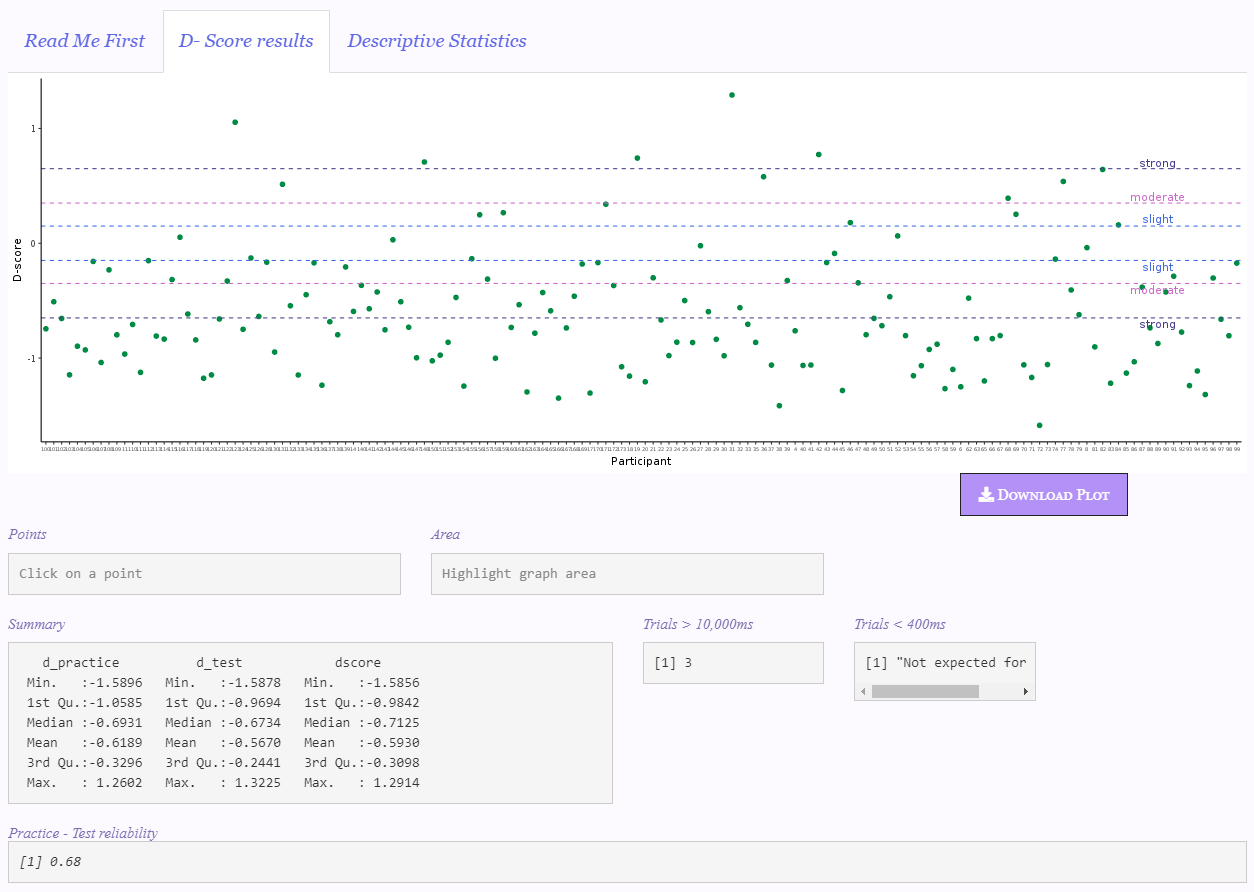
\includegraphics[width=0.8\textwidth]{resultsApp.png}
	\caption{DscoreApp results panel.}
	\label{fig:dscoreapp}
\end{figure}
%
Both descriptive statistics of the results and their graphical representation are available at the same time, and they change interactively as users change the configuration in ``Input panel''. The \texttt{Summary} box reports the descriptive statistics of the $D_{\text{practice}}$, $D_{\text{test}}$, and the actual \emph{D-score}. The \texttt{Trials > 10,000ms} box reports the number of trials discarded because of a slow latency (if any), while the \texttt{Trials < 400ms} box reports the trials discarded because of fast response times. This box is populated only when a \emph{D-score} with fast trials deletion is selected, otherwise the ``Not expected for this D'' label is displayed. The \texttt{Practice-Test reliability} box contains the IAT reliability computed as the correlation between associative practice and associative test blocks across participants \cite{gaw2017}.

DscoreApp provides users with different options for the graphical representation of the results (Figure \ref{fig:dscoregraph}), at both the individual (Figure \ref{fig:point}) and sample level (Figure \ref{fig:hist}, \ref{fig:dens}, \ref{fig:histdens}). 
%
\begin{figure}[h!]
	\centering 
	\begin{subfigure}{0.4\linewidth}
		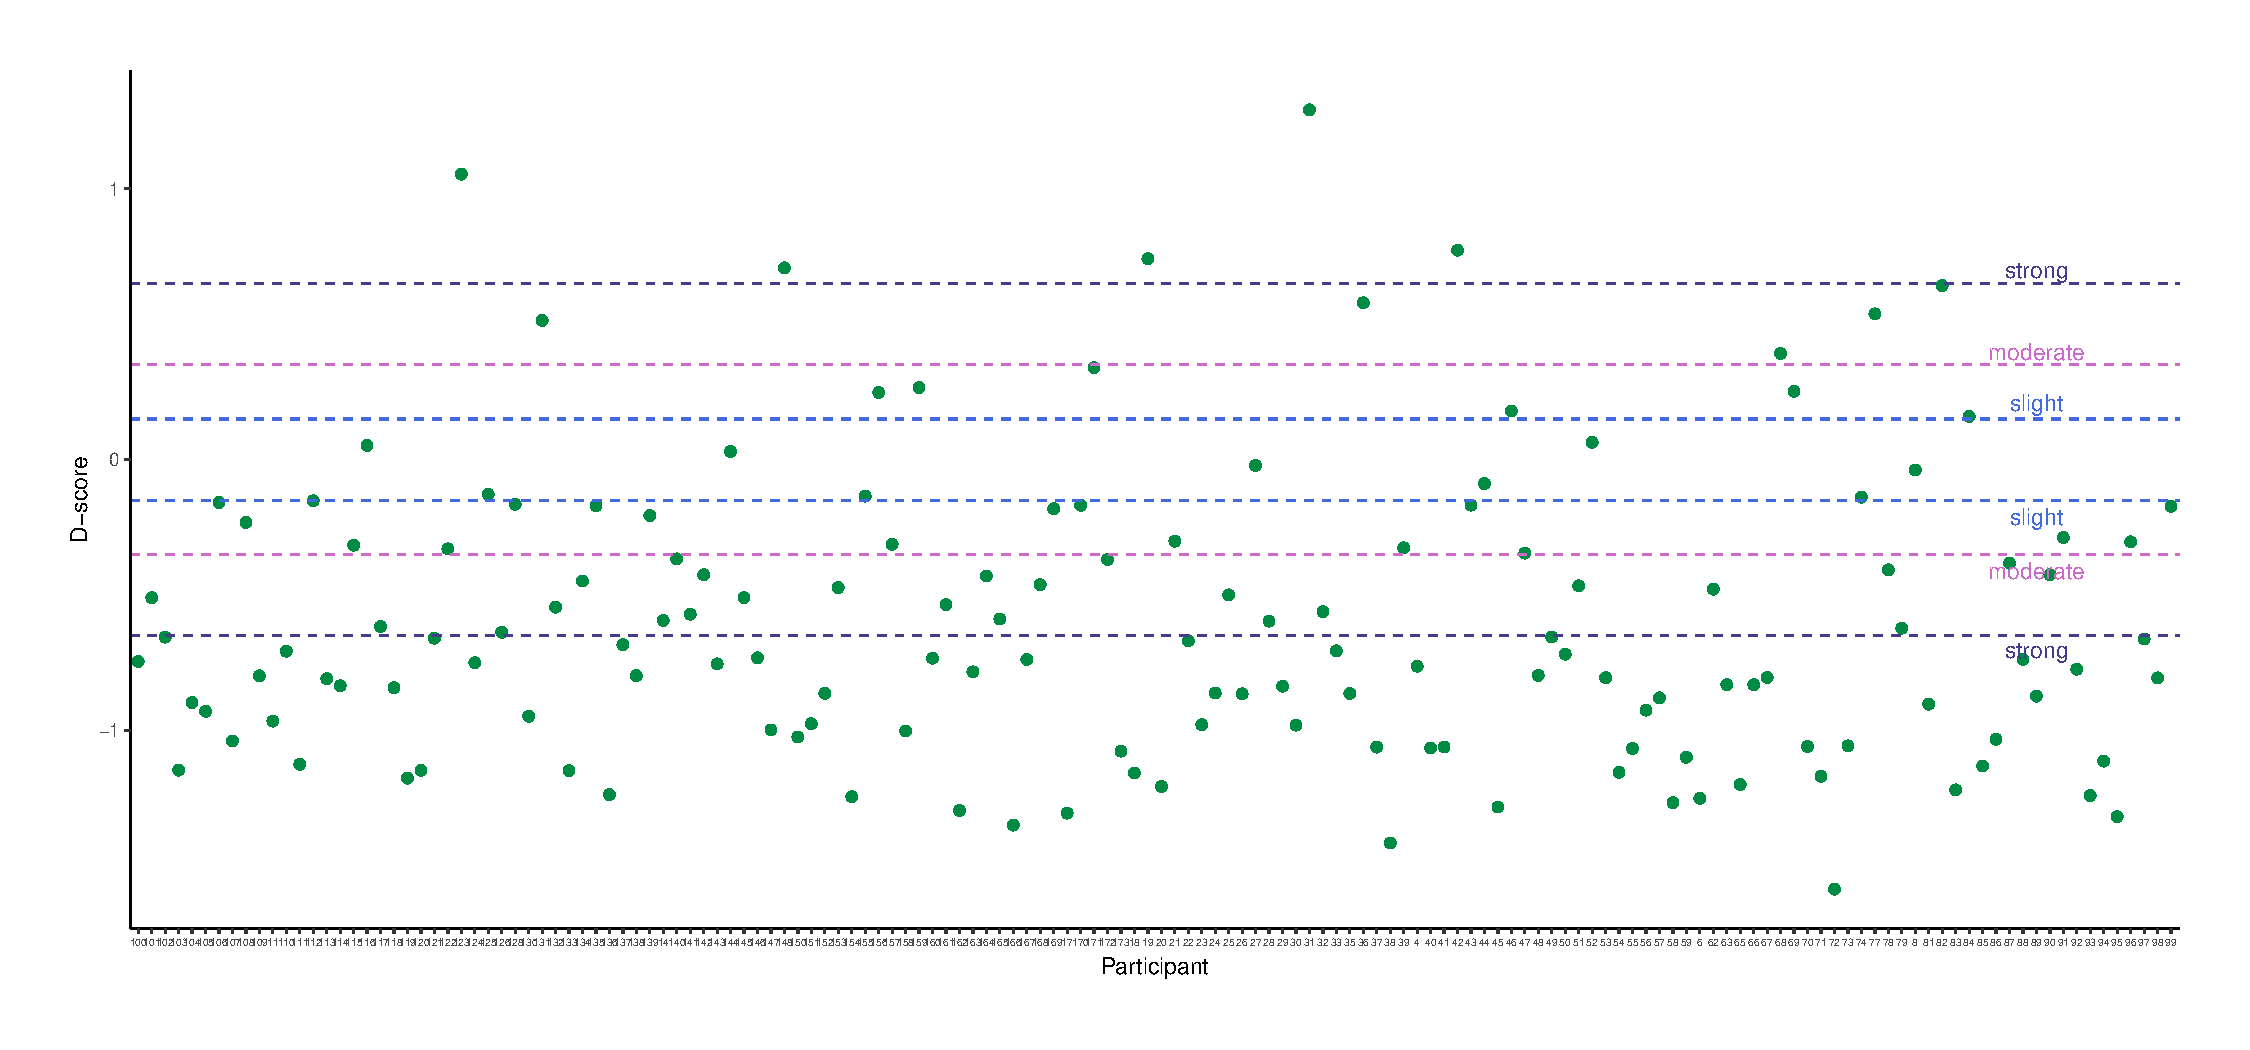
\includegraphics[width=\linewidth]{PointDefaultDscore3.pdf}
		\caption{Points graph.}
		\label{fig:point}
	\end{subfigure}
	\begin{subfigure}{0.4\linewidth}
		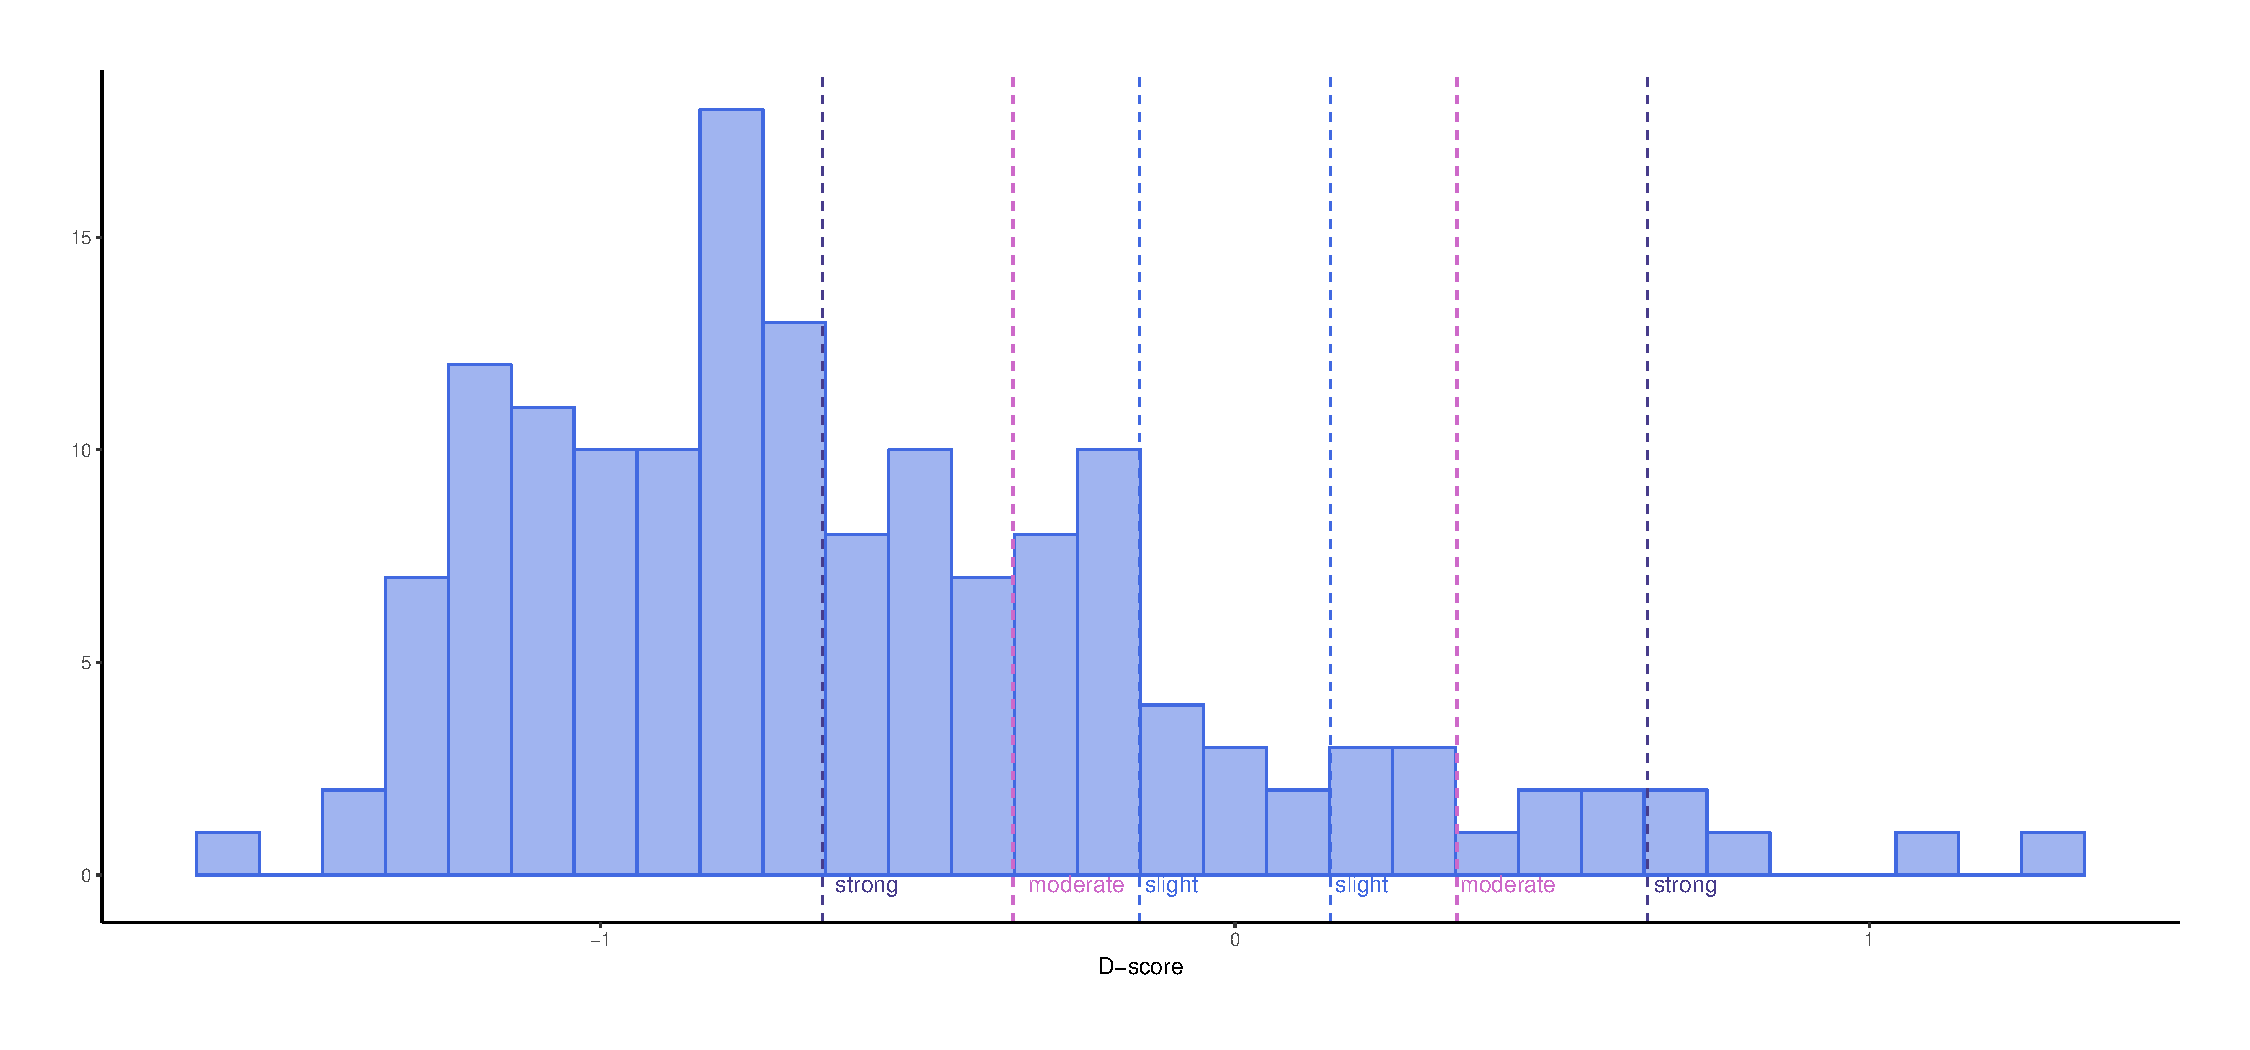
\includegraphics[width=\linewidth]{HistogramDscore3.pdf}
		\caption{Histogram.}
		\label{fig:hist}
	\end{subfigure}
	\begin{subfigure}{0.4\linewidth}
		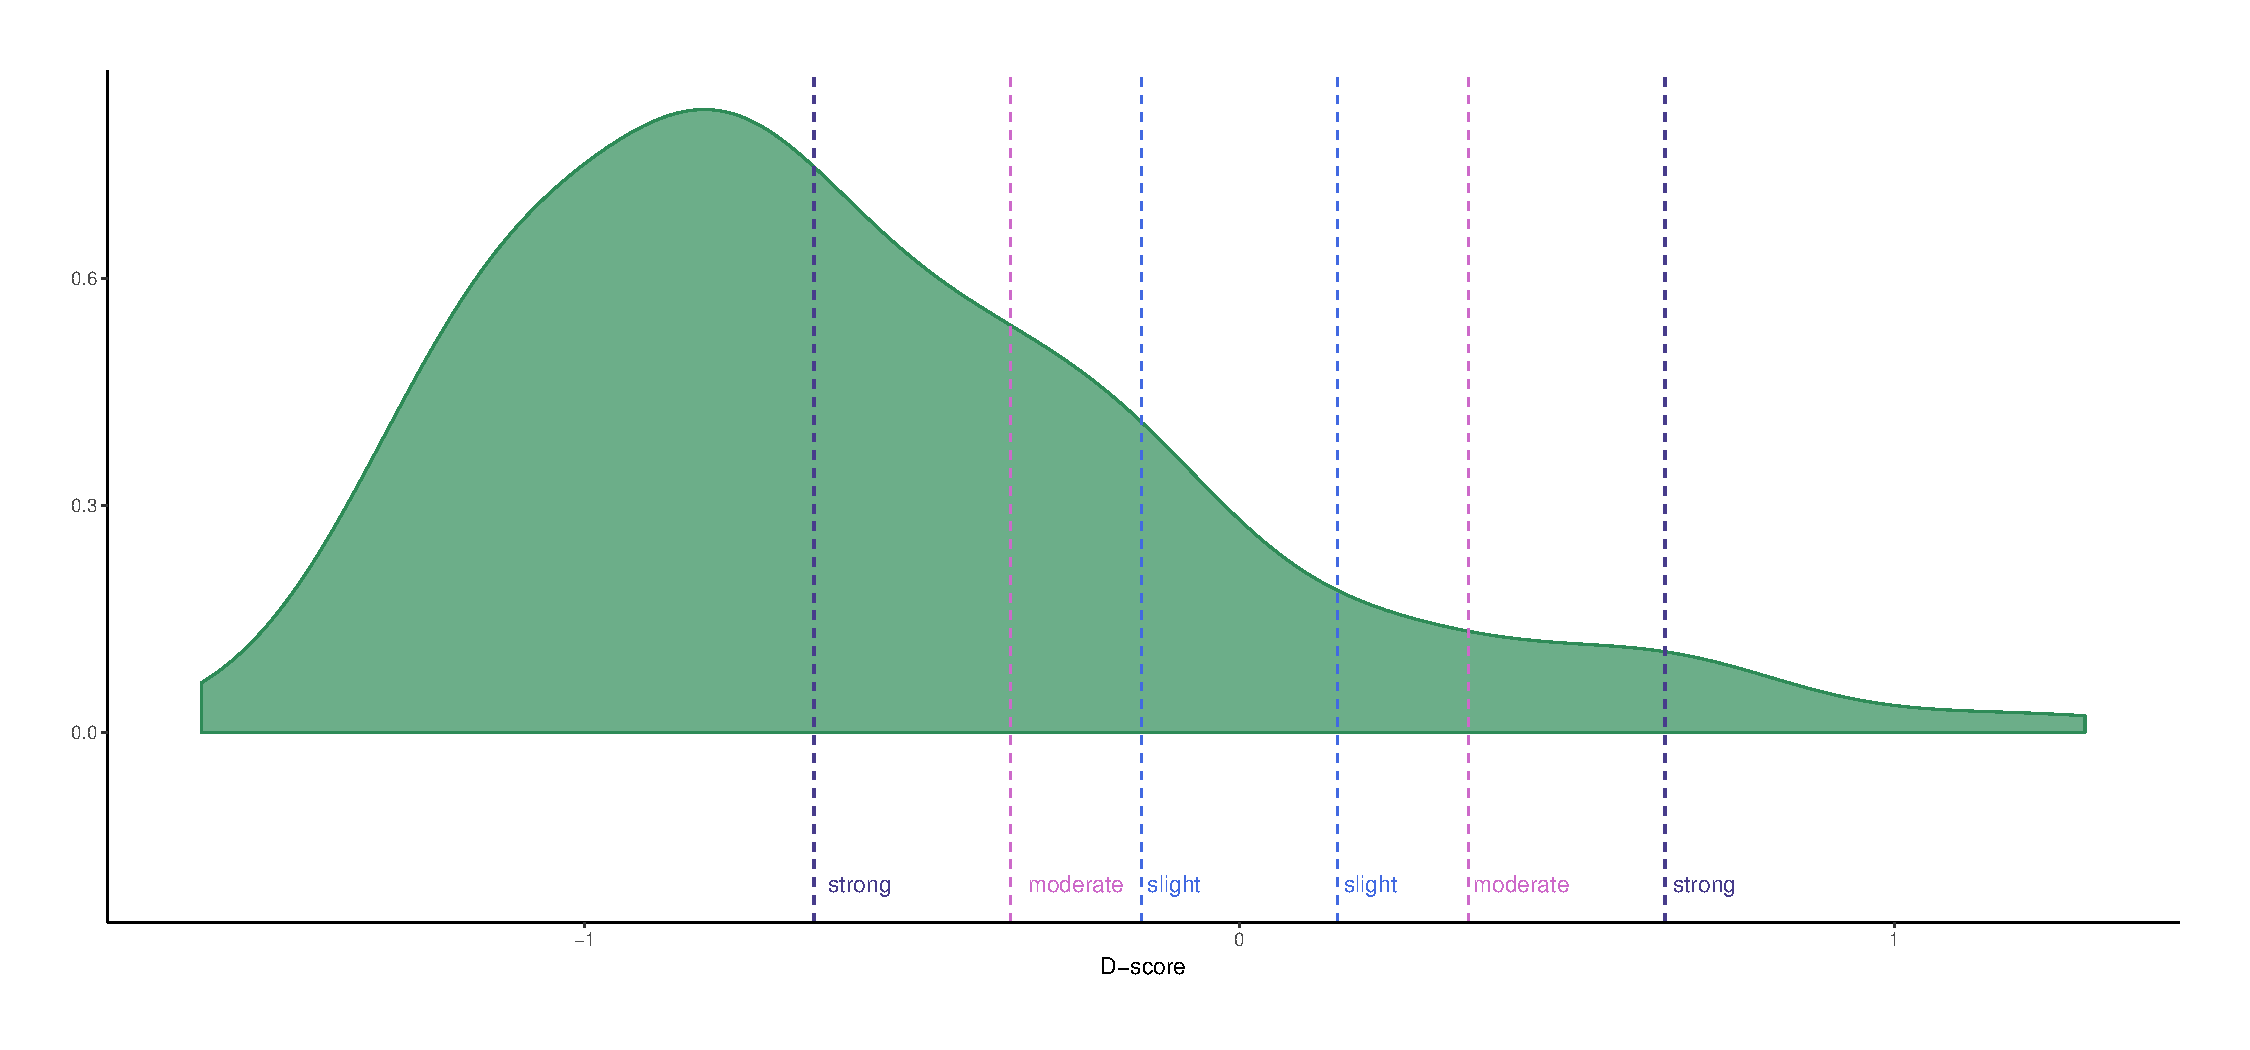
\includegraphics[width=\linewidth]{DensityDscore3.pdf}
		\caption{Density.}
		\label{fig:dens}
	\end{subfigure}
	\begin{subfigure}{0.4\linewidth}
		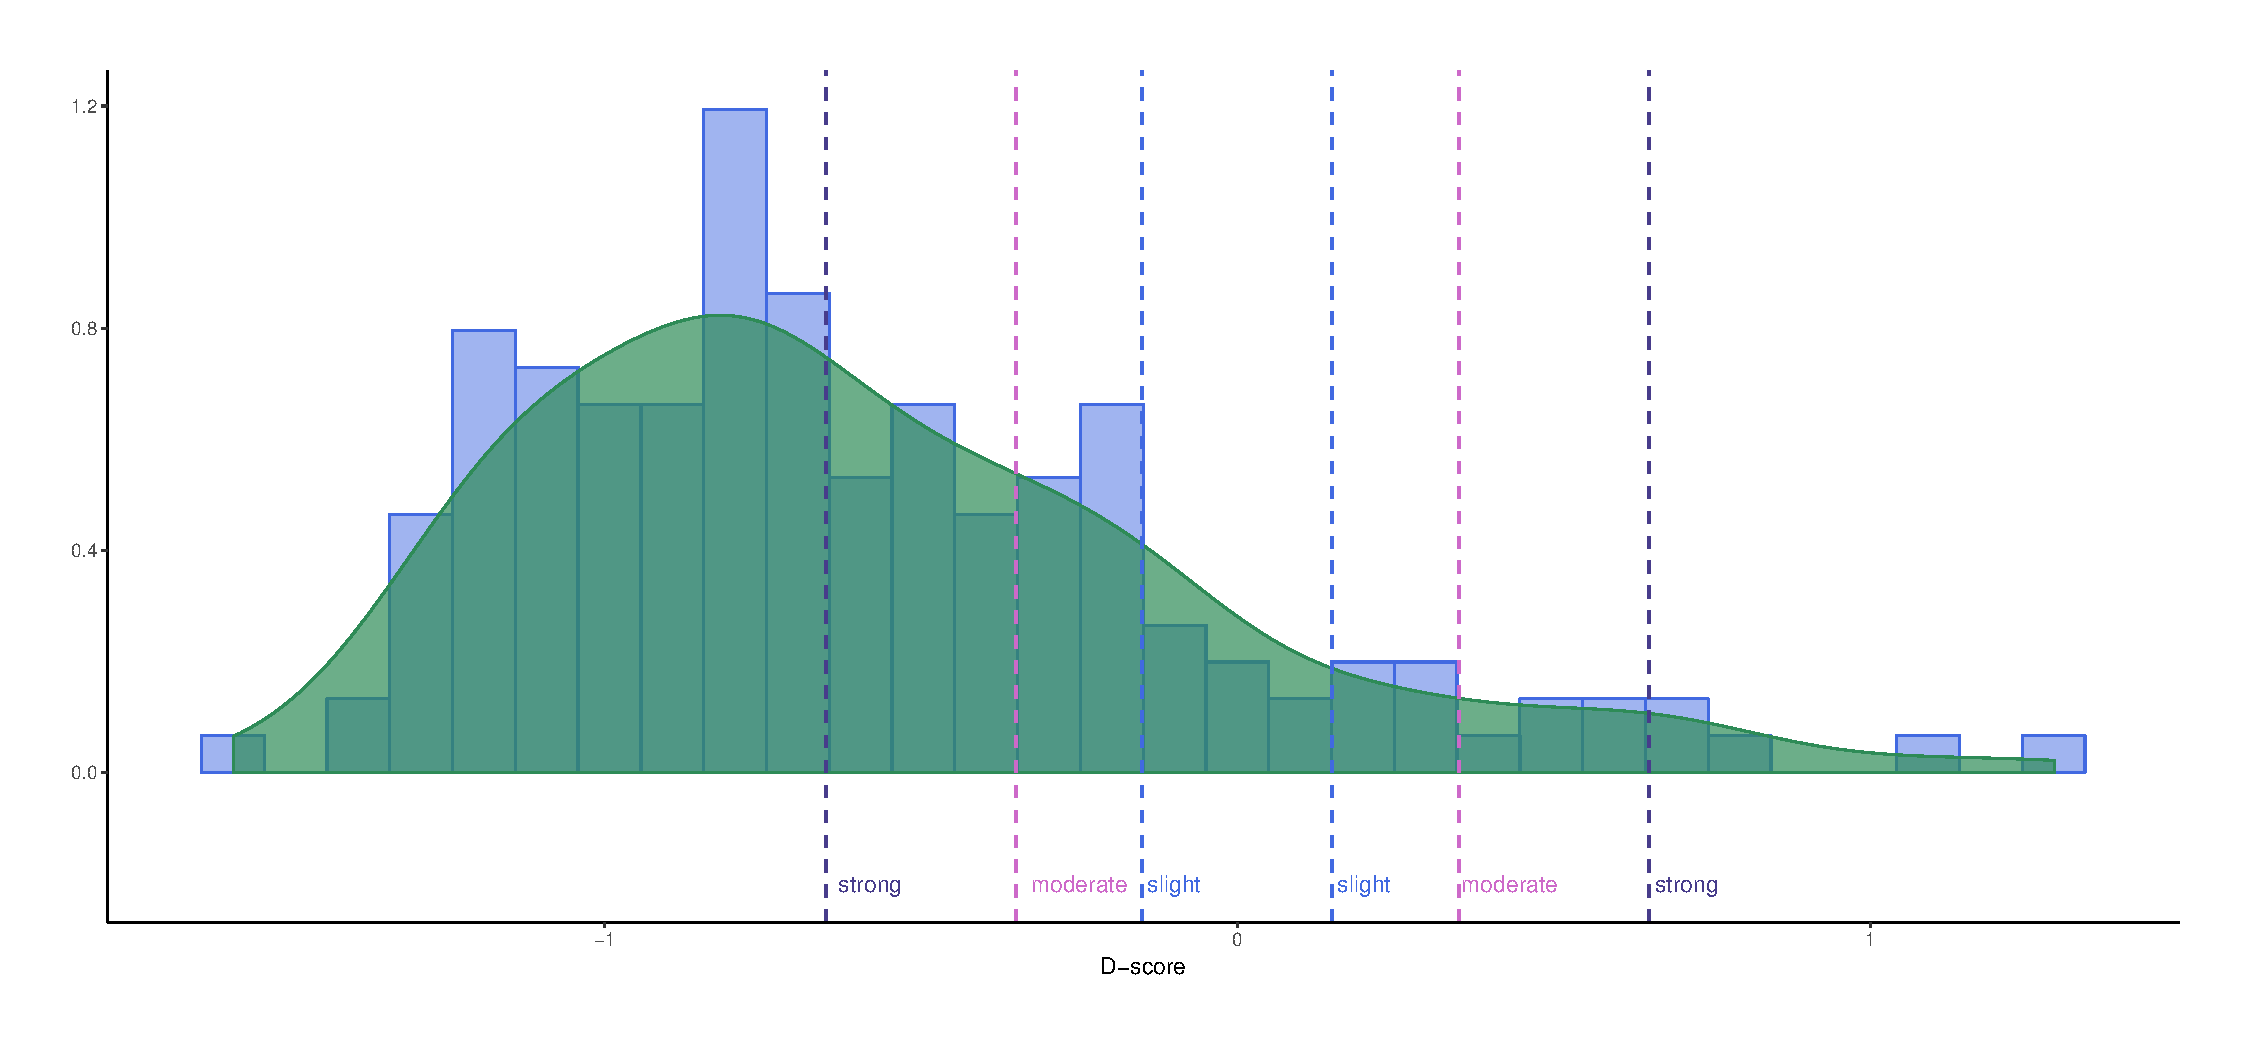
\includegraphics[width=\linewidth]{HistDensDscore3.pdf}
		\caption{Histogram and Density.}
		\label{fig:histdens}
	\end{subfigure}
	\caption{\label{fig:dscoregraph} Available graph representation}
\end{figure}

Graphical representation is a convenient way to identify extreme scores or particular response pattern. Since it might be difficult to link a particular point (or points area) in the graph with the corresponding participants' IDs in the data set, DscoreApp comes with two handy tools designed to access the respondents' IDs from the graph. By clicking on a point in the graph, the ID of the participant that corresponds to the selected point, and his/her \emph{D-score}, appears in the \texttt{Point} box (see Figure~\ref{fig:dscoreapp}). By highlighting an area of the graph, the IDs of participants included in the area, along with their \emph{D-score}s appears in the \texttt{Area} box (see Figure~\ref{fig:dscoreapp}).  

All the graphical representations are downloadable in a .pdf format.

\chapter{Formal modeling}

In this chapter, a brief overview of the models proposed for modeling IAT data is provided, and their advantages and drawbacks are highlighted. 
Some of these models are aimed at investigating the cognitive processes that are playing a role in the IAT by exploiting all the information that can be gathered from the accuracy responses (Section \ref{sec:multimodel}), while others are concurrently considering the accuracy and response times for delving deeper on the implicit associations driving the performance (Section \ref{sec:timeacc}). One common drawback of these models is that they are not able to provide information at the level of the individual stimulus.

The advantages of Rasch modeling of the IAT data by means of the Many Facet Rasch Modeling (MFRM) are illustrated in Section \ref{sec:mfrm}. Although this approach can provide stimulus--specific information, it also comes with drawbacks that cannot be ignored. 

%Different models have been proposed for getting a better understanding of the IAT effect. Some of these models, like the Quad Model \cite<Section \ref{sub:quad}>{Conrey2005} or the ReAL Model \cite{Meissner2013}, consider only the accuracy responses, while other models, like the Diffusion Model \cite<DM;>{Klauer2007} or the Discrimination-Association Model \cite<DAM;>{stefanutti2013}, simultaneously account for both accuracy and time responses. These models provide useful information at either the sample level (Quad model and ReAL model) or the respondent level (DAM and DM). DM and DAM also inform about the stimuli, but the information is provided at the level of stimuli categories and not at that of individual stimuli. 

%Nevertheless, fine-grained information at the stimuli level would allow for testing whether individual stimuli are actually recognizable as prototypical exemplars of their own reference categories. Furthermore, the investigation on the contribution of each stimulus to the IAT effect would help in shedding a light on the meaning of the implicit measure itself.
\newpage
\section{Multionomial Models}\label{sec:multimodel}
\subsection{Quad Model.}\label{sub:quad}
The Quad model \cite{Conrey2005} is a multinomial model introduced for distinguishing the contribution of automatic and controlled process in driving the respondents' performance in the IAT. Specifically, Quad model is aimed at highlighting the contribution of four qualitatively different processes defined by different levels of automaticity and/or controllability.  It is completely based on accuracy responses, and it exploits the logic of response compatibility. Response compatibility is the assumption on which the IAT rests, namely, that responses are more accurate and faster in the condition compatible with respondent's automatic association. 
The activation, or lack of thereof, of the four processes contributes to the overt response in the IAT. 
The observed probability of a correct response to a particular category of stimuli is the starting point for estimating the four parameters. The sum of the probabilities associated with a response is the total probability of that response. 

The likelihood that an automatic association is activated by a category of stimuli is captured by the \emph{association activation} parameter (AC), which expresses the most automatic component of the model and it is directly related to the strength of the association activated by the stimulus. The stronger the association, the more likely it will be activated by the triggering stimulus. 

The probability of giving the correct response also depends on the ability of identifying the actual correct response, and the \emph{discriminability} parameter (D) expresses the likelihood that the correct response (i.e., the correct category to which the triggering stimulus belongs) is identified.

If a negative automatic association is activated by the stimulus (e.g., racial prejudice), the respondent might try to fake the response in a socially desirable way. This process is captured by the \emph{overcoming bias} parameter (OB), which expresses the likelihood that an activated bias is overcome in favor of a deliberate, and probably more desirable, response. 

Parameters D and OB are the parameters that are mostly influenced by motivation and that mostly depend on the availability of cognitive resources to be effective. 

Finally, the Quad model takes into account the chance that, in absence of any other of the processes, the responses are influenced by any response bias, which might also be tendency to respond with the left response key. The \emph{guessing} parameters (G) defines the likelihood that this response bias is activated and drives the responses. 

%The first process considered is the likelihood that an automatic association is triggered by a stimulus (AC parameter). This process represents the automatic component of the model. The other three processes involved in the model represent processes with different degrees of controllability. One of them, namely defines the likelihood that the correct response Another process involved in the response is likelihood that the correct response is identified (D parameter). Besides the automatic activation of the association, also the likelihood that the respondent is able to overcome the automatic bias (OB parameter) plays a role. Finally, the likelihood that, in absence of any other information, a general response bias will guide the response will also be accounted for (G parameter). 

Despite this model results in a distinction between automatic and controlled processes taking place during the IAT, and can hence provide a better understanding of the IAT functioning, it presents some drawbacks. Since it is based solely on accuracy responses, it can present at least two issues. Firstly, the IAT is designed to be an extremely easy task, hence the proportion of correct responses is extremely high. Secondly, this model is neglecting all the information that can be gathered from the responses times, and that can potentially lead to further and more detailed results. Finally, all the parameters are at the sample level. 
 
%According to the Quad Model, the accuracy performance at the IAT depends on four qualitatively distinct processes: (i) the automatic activation of an association triggered by a stimulus, (ii) the ability to discriminate the correct category to which the stimulus belongs, (iii) the ability to overcome automatically activated associations, and (iv) any response bias (e.g., the tendency to respond with the right response key) that may drive the response in absence of any other process. 



\subsection{ReAL Model}\label{sub:real}

The ReAL model \cite{Meissner2013} is a multinomial processing tree model aimed at disentangling the different processes involved in the IAT. The assumption at the base of this model is that part of the respondents' performance is not ascribable to their automatic association, but it is due to strategies undertaken during the administration. Thus, this model should be able to mathematically distinguish between actual attitude associations and recoding strategies. 

As the Quad model, the ReAL model is based on the accuracy responses. Three processes are assumed to drive the correct and incorrect response pattern in the IAT, according to the IAT associative condition. Specifically, in the condition compatible with the automatic association of the respondent, all three processes are supposed to play a role, while in the incompatible condition only two of them are driving the response pattern. 

By assuming that attitude objects can activate evaluative associations, a Re-coding process (i.e., \emph{Re}) can intervene in the compatible condition. This means that the categorization tasks is reduced from four categories to two categories by exploiting the evaluative characteristics of the attitude objects. In the compatible condition, the object stimuli can be sorted by using their attribute characteristics (i.e., being evaluated as \emph{Good} or \emph{Bad}).  The Re-coding process can facilitate the task in the compatible condition, while it can interfere with it in the opposite one. If the Re-coding processes is not activated, then the Label-based (i.e., \emph{L}) process drives the response. This process represents the controlled search for the label representing the category to which the stimulus belongs. When neither the Re-coding process nor the Label-based one are involved, the Evaluative associations (i.e., \emph{A}) of the object categories can actually drive the response.

Evaluative associations and label based processes take place in both IAT associative conditions. Recoding takes place only in the condition that is consistent with the respondent's automatic activated association. 


\section{Time and Accuracy models}\label{sec:timeacc}
\subsection{Diffusion Model}
The first application of the Diffusion Model \cite<DM;>{ratcliff1978} to the IAT data can be found in \citeA{Klauer2007}. As the Quad and the ReAL models, also the DM is aimed at disentangling the contribution of different process contributing to performance at the IAT. Additionally, since DM maps accuracy and response times on the same metric, it can exploit the information deriving from both type of responses.  

The assumption on which the DM rests is that decisions in two-choice tasks like the IAT are based on processes of information accumulation during time. Once the amount of information reaches the thresholds for determining the responses, the response associated to that threshold is given. 

According to DM, there are four main components that intervene in information processing. The first one is the speed with which the information is accumulated. This components is expressed by the \emph{drift rate} (i.e., parameter $v$), which quantifies the direction and speed with which the information is accumulated. It determines both the respondent's accuracy and time performance. 

The thresholds defining the amount of information needed for giving a response are another component of the DM. Each threshold is associated with a response, namely the correct (stimulus correctly sorted in the category) and incorrect (stimulus incorrectly sorted in the incorrect category) one. This component si expressed by the \emph{separation} parameter (i.e., parameter $a$), which quantifies the amount of evidence in favor of one versus the other response. Clearly, the amount fo information that needs to be accumulated depends on the starting point from which the accumulation process starts, that is, the \emph{starting point} of information accumulation. This parameter informs about the response bias towards one of the two response thresholds. 

Finally, there is also a non-decision component involved in the response process. This component refers to the time used for actions that are not directly implicated in the response process, like the encoding of the stimuli or the response execution itself. Parameter $t_0$ represents the contribution of the non-decision component to the response processes. 

According to the DM, attitudes enter the IAT, and hence guide the responses, through the object stimuli. Specifically, the automatic association positively influences the \emph{drift-rate} in the compatible condition (i.e., faster and more accurate responses), while it negatively influences the \emph{drift-rate} in the incompatible condition (i.e., slower and less accurate responses). Consistently with the Recoding strategy illustrated in the ReAL model, the faster and more accurate responses in the compatible condition result from the use of the positive/negative valence of the object stimuli for their categorization, hence avoiding the task-switch cost from attribute to target. 

Since the DM provides the distribution of both correct and incorrect responses, it results in a detailed information on the IAT functioning and on the respondents' performance. However, for doing so, it needs a high proportion of incorrect responses, which is quite difficult to observe in an IAT. One solution to make the respondents commit more mistakes is to add more trials to the each associative condition. Moreover, DM is separately applied to each entire critical block, without distinguishing between the different stimuli categories. This also implies that parameters values estimated from different block cannot be compared. 
 
\subsection{Discrimination-Association Model}\label{sec:DAM}
The Discrimination-Association Model \cite<DAM;>{stefanutti2013} has been specifically developed for the analysis of IAT data, with the aim of separating automatic from controlled processes while accounting for both accuracy and time responses.  

DAM decomposes the IAT effect into three processes, namely stimuli discrimination, automatic association, and termination criteria. Stimuli discrimination informs about the functioning of the stimuli and, specifically, whether the stimuli can be easily recognized and categorized into the correct category. However, this information is not at the level of the individual stimulus but at that of the stimuli category. The process that mostly regards individual differences is the automatic association one, which provides information about the association between the evaluative dimension and the object categories. This information allows for a better understanding the meaning of the IAT measures. Consider again the Coke-Pepsi IAT in Section \ref{sec:iat}. A positive \emph{D-score} on this IAT might both indicate faster responses in associating Coke/Good, Pepsi/Bad, or both. In any case, a positive score is obtained, but with different meanings. If the Coke/Good association are driving the responses, it means that it is more the preference for Coke to guide the performance. Otherwise, if the associations Pepsi/Bad are driving the responses, it is more the dislike for Pepsi, than the preference for Coke, to determine the performance. However, the \emph{D-score} cannot distinguish between the two distinct automatic associations, while DAM can, providing a better understanding of the IAT measures.    
Finally, termination criteria represents the amount of information that must be accumulated before a response is given. It can be interpreted as either task difficulty or individual cautiousness in giving the responses.

DAM provides useful information on the IAT functioning, and it also overcomes some of the issues of DM. For example, since the DAM assumes that correct and incorrect responses are deriving from different processes, reliable parameters estimates can be obtained even when no error responses are present. Besides, DAM is applied on the entire set of IAT blocks. 

However, also DAM presents some shortcomings. Firstly, the information on stimuli functioning regards only the stimuli categories and not the individual stimulus. Secondly, since the termination criteria can be interpreted as either a property of the task (i.e., difficulty) or an individual characteristic (i.e., respondent's cautiousness), it is confounding the distinct contribution of the task and that of the respondent in determining the responses. 
Finally, DAM is based on Poisson processes, and it is actually an extension of the Poisson race model. The average user of the IAT tends not to be familiar with that kind of models, and might find the interpretation of the parameters, or the model itself, utterly complicated, without noticing the clear advantages deriving from this approach. 

\section{Rasch Modeling} \label{sec:mfrm}

By applying the Rasch model \cite[See Chapter \ref{sec:rasch}]{rasch1960} to IAT data it is possible to disentangle both respondents and stimuli contribution to each response process. The detailed and fine-grained information at both levels can be used to shed a new light on the meaning of the IAT measure. The information at the stimuli level can be used to test whether IAT stimuli are recognizable as prototypical exemplars of the category they are supposed to represent. Moreover, this information allows for investigating the contribution of each stimulus to the IAT effect, which can in turn help in understanding the meaning of the IAT measure. The information at the respondents' level might help in clarifying whether there are any artifacts in the IAT procedure that can affect respondents' performance, and hence the resulting IAT effect. 

The Many Facet Rasch Model \cite<MFRM;>{linacre1989} has been successfully applied to the discretized IAT time responses, providing interesting insights on the functioning of the IAT stimuli \cite{anselmi2011, anselmi2013, anselmi2013a}. The information obtained on the stimuli was used for disentangling the automatic associations that mostly contribute to the IAT effect. In the Rasch model, the likelihood of a correct responses depends on both the respondent's ability $\theta$ and the stimulus difficulty $b$. The MFRM is an extension of the classic Rasch model in which other sources of systematic variability (i.e., \emph{facets}) are accounted for the correct response. The IAT associative condition can be considered as a facet of the MFRM, and, as such, it allows for obtaining condition--specific stimuli parameters. For instance, by comparing the condition--specific stimuli parameters, \cite{anselmi2011} found a positive primacy effect, for which the IAT effect was mostly driven by positive stimuli. By drawing on this result, the authors suggested that the implicit preference for Caucasian people over African people that is often observed in Caucasian respondents could be expression of in-group favoritism rather than out-group derogation. 

%Despite the useful that can gathered from its application to IAT responses, the MFRM presents some drawbacks. Firstly, the MFRM was applied on the discretized time responses of the IAT. The discretization process can lead to a potentially large loss of information, that can be avoided by considering the response times in their continuous nature. Moreover, as it is, the MFRM cannot account for the cross-classified structure of the IAT, and, as such, it might result in biased estimates due to the non-independence of the observations. Finally, to obtain the condition--specific stimuli estimates, it was assumed that the difficulty of the IAT conditions was not changing across respondents, and hence the individual differences were completely overlooked. 


Despite Rasch modeling of the IAT data provides interesting insights on the IAT functioning, it also presents some shortcomings. Firstly, by discretizing the response times, a part of the information that can be retrieved is lost, and the variability of the responses is reduced. Secondly, by applying the MFRM to the IAT data, its fully-crossed structure is not accounted for, hence the non-independence of the observations was not accounted for. Thus, the estimates obtained through the application of this model might result biased by the influence of unwanted and uncontrolled error variance. Finally, in the application made by \citeA{anselmi2011}, the focus was on the functioning of the stimuli between the two associative conditions. To obtain the condition--specific estimates, it was assumed that the difficulty of the two conditions was assumed to be the same for all respondents. Consequently, it was not possible to investigate the respondents' individual differences in performing the IAT. 


\chapter{Rasch model model and log-normal model}
In this Chapter, Rasch model and log-normal models are briefly outlined. The advantages of using Linear Mixed Effect Models on IAT data are then discussed, as well as how to obtain the Rasch model and the log-normal model parameters estimates from the (Generalized) Linear Model, also considering the extension to multidimensional data. 

\newpage

\section{Rasch Model} \label{sec:rasch}

According to the Rasch model, the likelihood of a respondent $i$ to endorse the correct response on a item $j$ can be expressed as the function of the respondents ability $\theta$ and the item difficulty $b$. The correct response will be endorsed when the respondent ability is higher than the item difficulty. Vice-versa, an incorrect response will be endorsed when the respondent ability has a lower ability than the difficulty of the item. When the respondent's ability is equal to the stimulus ability, the respondent probability of endorsing the correct response will be equal to his/her probability of endorsing the incorrect response. 

The Rasch model can be formally expressed as follow:
%
\begin{equation}\label{eq:rasch}
P(x_{ij} = 1|\theta, b) = \frac{exp(\theta_i - b_j)}{1 + exp(\theta_i - b_j)},
\end{equation}
%
where $x_{ij}$ is the accuracy response of respondent $i$ on item $j$. 

In the IAT case, the correct response to each stimulus is given by the correct categorization of the stimulus in the category to which it belongs. Respondent's ability can hence be considered as the ability to correctly recognize the correct category to which the stimulus belongs and assign it to that category. Stimulus difficulty can be considered as the stimulus characteristics that are making it more or less recognizable as a prototypical exemplar of the category it is supposed to represent. 

The higher the value of $\theta_i$, the higher the respondent ability to sort the stimuli into the correct categories, and hence the higher the proportion of responses correctly identified. The higher the value of $b$, the more difficult a stimulus is, meaning that it is not easily identified as a prototypical exemplars of the category to which it belongs, and it hence gets a higher proportion of incorrect responses.

\section{Log-normal Model}

The discretization of the response times needed for the application of the MFRM (see Chapter \ref{sec:mfrm}) can be avoided by considering the normal distribution of the log-transformed response times. By doing so, it is possible to consider the response times in their continuous nature while obtaining a parametrization similar to Rasch parametrization by means of the log-normal model \cite{van2006}. 

According to the log-normal model, the log-time response of respondent $i$ on item $j$ can be expressed as a function of respondent's speed $\tau$ and stimulus time intensity $\delta$. Time intensity can be defined as the time each stimulus requires for getting a response, and it is strongly dependent on the characteristics of the stimulus itself \cite{van2006}. 

The log-normal model can be formally expressed as follow: 
%
\begin{equation}\label{eq:log}
f(t_{ij}| \tau_i, \delta_j) = \frac{1}{t_{ij}\sqrt{2\pi}}exp\left\{ -\frac{1}{2}[ln\;t_{ij} - (\delta_j - \tau_i)]^2 \right\},
\end{equation} 
%
where $t_{ij}$ is the response time of respondent $i$ on stimulus $j$. The person parameter $\tau$ describes the speed of the respondent; The larger the value of $\tau$, the smaller the amount of time the person needs to respond. Stimulus parameter $\delta$ is interpreted as the time a stimulus demands for getting a response (i.e., \emph{time intensity}); the larger the value of $\delta$, the more time is required by the stimulus to get a response. 

The relation between the stimulus parameter $\delta$ and the respondent parameter $\tau$, expressing the mean of the distribution of Equation (\ref{eq:log}), resembles the relation between the respondent parameter $\theta$ and stimulus parameter $b$ in the Rasch model (\ref{eq:rasch}).

\section{Linear Mixed Effects Models}

A Rasch approach to the analysis of the IAT data proven to be an efficient way to obtain stimuli parameters estimates leading to a deeper comprehension of the meausure itself. The use of a model considering the normal distribution of the log-time responses allows for considering the response time in their continuous nature and hence to overcome the issue of the loss of information due to the discretization for the application of the MFRM. Nonetheless, there is still something missing, that is, the cross-classified structure of the data is still not taken into account. 

To deal with the cross-classified structure characterizing both the IAT and the SC-IAT, the multilevel structure of the data must be considered as reflecting the random variability of the population from which the different levels are drawn \cite{Barr2013}. This can be done by considering the random variation of each level and by specifying it as a random effect \cite{Doran2007}. 

\subsection{(Generalized) Linear Model and Rasch Model}

A generalized linear model is a linear model in which the linear predictor for the $i$-th response is related to the expected value of the response, $\mu_i$ by an invertible link function \cite<\emph{g},>{mc1989}. The combination of the linear predictors can be written as $\eta_i = x_i\beta$, 
where $eta_i$ is the the combination of linear predictors and $x_i$ is the $i$-ith row of the \emph{observations} $\times$ \emph{predictors} model matrix \emph{\textbf{X}}, derived from the model and it covariates. 

The relationship between the linear predictors and the expected value of the response is as follows: 
%
\begin{equation}\label{eq:link}
	x_i\beta = \eta_i = g(\mu_i).
\end{equation}

The \emph{logit} is the natural link function for a binomial response \cite{mc1989}, defined as the logarithm of the odds (i.e., the ratio between the probability of a correct response and the probability of an incorrect response), for which: 
%
\begin{equation}
	\eta_i = g(\mu_i) = log\left( \frac{\mu_i}{1 - \mu_i}\right), 
\end{equation}

with inverse link: 
%
\begin{equation}\label{eq:inverse}
	\mu_i = g^{-1}(\eta_i) = \frac{exp(\eta_i)}{1 + exp(\eta_i)}.
\end{equation}

The structure of inverse of the \emph{logit} link function in Equation \ref{inverse} clearly allows for seeing the relationship with the Rasch model as expressed by the Model in Equation \ref{eq:rasch}.

\subsection{Extending to Multidimensional data}
To extend the generalized linear model to multilevel data, and hence to move from a GLM to a Generalized Linear Mixed Effect Model (GLMM), the linear combination of predictors $\eta$ must include both fixed effects $\beta$ and random effects $d$, such that: 
%
\begin{equation}
	\eta = X\beta + Zd,
\end{equation}

where $X$ is the \emph{observations} $\times$ \emph{predictors} model matrix, whereas $Z$ is the \emph{observations} $\times$ \emph{grouping factor}. Each component of the random effects $d$ is associated with a level of the grouping factor.  

At this point, the random variability of different grouping factors, being the type of items or the conditions of presentation, are included in the model matrix and are hence accounted for, and it is possible to obtain the Rasch model parameters by using the estimates of the fixed effects and the marginal modes of the random effects, or Best Linear Unbiased Predictors (BLUP). BLUPs are expressing the adjustment of each level of the random effects to the fixed effects. Formally, BLUPs are not parameters of the model themselves, and they are obtained after the estimation of the random effect parameters, that is, the expected variance of the specific level of the random effect.


\chapter{Models specification}

The (Generalized) Linear Mixed Effect models random structures are specified in this chapter. Form each of the illustrated random structure, different parameters for the Rasch and log-normal models. 

Since the IAT has a specific data structure, a Maximal Model was introduced. Nonetheless, the random structure of the Maximal Model is know to be too complex to fit on empirical data sets. Consequently, models with simpler random structures were specified starting by the random structure of the maximal model. A final overview of the Rasch and log-normal model that can be extracted from each of the random structures is presented. 

\newpage
\section{Maximal Model}

All the sources of variability in the IAT can be taken into account by specifying them in a model with the appropriate random structure, in which the error variance is decomposed into each of the sources of variation \cite<Maximal Model, MM;>{Barr2013}. The expected response $y$ for the observation $i = 1, \ldots, n$  for participant $j = 1,\ldots, J$ on stimulus $k = 1,\ldots, K$ in condition $l= 1,\ldots, L$ can be expressed by the following model:
%
\begin{equation}\label{maxmax}
y_{i} = \alpha + \beta_il_i + \alpha_{j[i]} + \alpha_{k[i]} +  \alpha_{j[i]}\alpha_{k[i]} + \beta_{j[i]}l_{i} + \beta_{k[i]}l_{i} + \epsilon_{i},
\end{equation}
with:
\begin{align}
(\alpha_{j} ,\beta_{j}) \sim  \mathcal{N}
\begin{pmatrix}
0,&
\begin{pmatrix}
\sigma_{\alpha_j}^2 & \sigma_{\alpha_j, \beta_j}^2 \\
\sigma_{\alpha_j, \beta_j}^2 & \sigma_{\beta_j}^2
\end{pmatrix}
\end{pmatrix},
\end{align}
\begin{align}
(\alpha_{k} ,\beta_{k}) & \sim  \mathcal{N}
\begin{pmatrix}
0,&
\begin{pmatrix}
\sigma_{\alpha_k}^2 & \sigma_{\alpha_k, \beta_k}^2 \\
\sigma_{\alpha_k, \beta_k}^2 & \sigma_{\beta_k}^2 
\end{pmatrix} 
\end{pmatrix},\\
(\alpha_{j } \alpha_{k}) & \sim  \mathcal{N}
\begin{pmatrix}
0,  \sigma_{\alpha_{j,k}}^2\\
\end{pmatrix},  \\
\epsilon & \sim N(0, \sigma^2).
\end{align}
%
The model Fixed effects are expressed by the fixed intercept $\alpha$ and the  fixed slope $\beta$. The fixed intercept $\alpha$ represents the expected average in the of the IAT condition and the fixed slope $\beta$ expresses the deviation from the first IAT condition. By summing up together, it is possible to obtain the estimate of the expected average in the second IAT condition. 


The between--respondents variability (i.e., difference in the response due to respondents individual differences) are accounted for by specifying their random intercepts $\alpha_{j[i]}$. Likewise, the between--stimuli variability is taken into account by specifying the stimuli random intercepts, represented by the term $\alpha_{k[i]}$. The variability due to the interaction between the stimuli and the respondents (i.e., respondents' individual reactions to each stimulus) is accounted for by the specification of the interaction effect between the stimuli and the respondents random intercepts (i.e., $\alpha_{j[i]}\alpha_{k[i]}$). 

The between--conditions variability is accounted for by specifying the respondents and stimuli random slopes in the associative conditions. The random slopes express the impairment/facilitation effect of the IAT condition on the respondents' performance or on the stimuli categorization. 

The MM, beyond being able to control for all the possible sources of random variation, is the one that allows for obtaining the higher amount of information. This model results in overall respondents' and stimuli parameters, as well as condition--specific respondents' and stimuli parameters. 

The comparison between respondents’ overall abilities and each of their two condition-specific parameters can inform about the bias in respondents' performance that is due to the IAT associative condition. Moreover, by computing the difference between the respondents' condition--specific parameters, it is possible to obtain a measure of this bias. 

Likewise, by comparing each stimulus condition--specific parameters with their overall parameter allows for investigating whether the stimuli categorization is somehow affected by the IAT associative condition. By computing the difference between the condition--specific stimuli parameters, a measure of the bias due to the IAT condition can be obtained. 

The MM is indeed providing numerous important information. Nonetheless, if the final aim is to obtain the Rasch and log-normal model parameters estimates from the IAT data, a model of such a complexity might not be needed. Moreover, a model of such a complexity is at risk of over-fitting or convergence failure \cite{Bates2015}, especially if the observed data do not have enough variability. 

Grounding on these considerations, models with simpler random structure were specified, starting from the random structure of the MM. Although interesting, it is not necessary to obtain both overall and condition--specific parameters for both the stimuli and the respondents. The model can hence be simplified by dropping the estimation of these parameters. Furthermore, the estimation of the interaction effect between the respondents' and the stimuli random intercepts can be dropped as well. Indeed, the estimation of this parameter requires a high variability in the data, and, if there is not, it brings to convergence failure. The estimation of this parameter should be added to the model only in those cases in which the error variance is still high after the estimation of all the other parameters \cite{Westfall2014}. For estimating the Rasch and the log-normal models parameters, either the respondents' or the stimuli parameters have to be centered at 0, otherwise the model is not identified \cite{Anselmi2011,Gelman2007}.


\section{Models random structure}

Three models for the accuracy responses (Rasch models) and three models for the log-time responses were specified. The random structures of these models were the same, besides the assumption on the error term $\epsilon$. This parameter was assumed to follow a logistic distribution for the accuracy models ($\epsilon \sim \mathcal{L}(0, \sigma^2)$) and a normal distribution for the log-time models ($\epsilon \sim \mathcal{N}(0, \sigma^2)$). 

Since the random structure is the same, and the only things that are changing are the assumptions on the error term and the dependent variable (either the accuracy or the log-time responses), only the equations for the specification of the accuracy models for the estimation of the Rasch models parameters are reported. The parameters of the log-normal model obtained through the application of the log-time models are commented as well. For both the accuracy and the log-time models, the fixed intercept $\alpha$ is set at 0, so that the estimates $\beta$ of the fixed effect of the associative condition can be interpreted as the expected proportion of correct responses in each condition (for the accuracy models) and as the expected average response time in each condition (for the log-time models) 

In Model 1, the within--respondents between--conditions variability and the between--stimuli variability are accounted for by specifying respondents' random slopes in conditions and stimuli random intercepts, respectively:
%
\begin{equation}\label{Accuracy1}
y_{i} = logit^{-1}(\alpha + \beta_il_i + \alpha_{k[i]} +  \beta_{j[i]}l_{i} + \epsilon_{i}),
\end{equation}
with:
\begin{align}
\beta_{j} \sim  \mathcal{N}
\begin{pmatrix}
0,&
\begin{pmatrix}
\sigma_{\beta_{jl_1}}^2 & \sigma_{\beta_ {jl_1}, \beta_{jl_2}}^2 \\
\sigma_{{\beta_{jl_1}}, \beta_{jl_2}}^2& \sigma_{\beta_{jl_2}}^2
\end{pmatrix}
\end{pmatrix},
\end{align}
\begin{align}
	\alpha_k \sim \mathcal{N} (0, \alpha_k^2).
\end{align}
%
The random structure of Model 1 results in condition--specific respondents' estimates and overall stimuli estimates. The condition--specific ability parameters of the Rasch model $\tau_{jl}$ are expressing the respondents' ability to perform the categorization task according to the associative condition. The higher the value of $\theta_{jl}$, the higher the ability of the respondent to perform the categorization task in the specific condition, and hence the higher the proportion of stimuli correctly categorized in that condition. Similarly, the condition--specific respondents' speed parameters $\tau_{jl}$ of the log-normal model are expressing the speed with which the respondents' are performing the categorization task in the specific associative condition. The lower the valued of $\tau_{jl}$, the higher the speed of the respondent, and hence the the lower the time needed for categorizing the stimuli. For both the Rasch and the log-normal models, the condition--specific respondents' parameters allow for testing whether there is an effect of the IAT associative condition on the respondents' accuracy or time performance, respectively.  Moreover, by computing the difference between the respondents' condition--specific parameters it is possible to obtain a measure of the bias in the performance due to the associative condition. The overall stimuli estimates, either easiness $b_{k}$ or time intensity $\delta_k$, can inform about each stimulus representativeness of its alleged category. The higher the easiness parameter $b$, the easier the stimulus is, meaning that it is easily recognizable as belonging to its category. The lower the value of the time intensity parameter $\delta_j$, the lower the time each stimulus needs to be categorized. 
The random structure of this model should be preferred when there is a low within--stimuli between--conditions variability, which can already indicate that the functioning of the stimuli does not change across conditions. 

In Model 2, the within--stimuli between--conditions variability and the between--respondents variability are taken into account by specifying stimuli random slopes in the associative conditions and respondents random intercepts, respectively: 
%
\begin{equation}\label{Accuracy2}
y_{i} = logit^{-1}(\alpha + \beta_il_i + \alpha_{j[i]} +  \beta_{k[i]}l_{i} + \epsilon_{i}),
\end{equation}
with:
\begin{align}
\beta_{k} \sim  \mathcal{N}
\begin{pmatrix}
0,&
\begin{pmatrix}
\sigma_{\beta_{kl_1}}^2 & \sigma_{\beta_ {kl_1}, \beta_{kl_2}}^2 \\
\sigma_{{\beta_{kl_1}}, \beta_{kl_2}}^2& \sigma_{\beta_{kl_2}}^2
\end{pmatrix}
\end{pmatrix},
\end{align}
\begin{align}
	\alpha_{j} \sim  \mathcal{N} (0, \sigma_{\alpha_j}^2). 
\end{align}

The random structure of Model 2 results in condition--specific stimuli parameters and overall respondents' parameters.  The condition--specific easiness parameters $b_{kl}$ are expressing the characteristics of the stimuli making them more easy to sort in the correct category according to the specific associative condition. The higher the value of $b_k$ in one condition, the easier the stimulus in that condition. This means that the stimulus is sorted more easily when it is associated with the stimulus category of that condition than in the other one. Likewise, the condition--specific time intensity parameters $\delta_{kl}$ are expressing the characteristics of the stimuli for which they are obtaining faster responses according to the associative condition. If a stimulus shows a higher $\delta_{k}$ parameter in one condition than in the other, it means that it obtained faster responses when it was associated with the stimuli category in the former condition than in the latter one. For both the Rasch and the log-normal models, the condition--specific stimuli parameters allow for testing the associative condition in which the stimuli are presented is influencing their functioning. Moreover, by computing the difference between the condition--specific parameters it is possible to obtain a measure of the bias due to the associative conditions, hence providing information on the contribution of each stimulus to the IAT effect. 
The overall respondents' parameters, either ability $\theta{jl}$ or speed $\tau_{jl}$, are giving a general information regarding the respondents' performance. 
The random structure of Model 2 should be preferred when a low within--respondents' between conditions variability is observed, which can already indicate that respondents' performance is not affected by the IAT associative condition. 

In Model 3, used as a Null model, between--respondents variability and between--stimuli variability were specified as respondents and stimuli random intercepts, respectively:
%
\begin{equation}\label{AccuracyMin}
y_{i} = logit^{-1}(\alpha + \beta_il_i + \alpha_{j[i]} +  \alpha_{k[i]} + \epsilon_{i}),
\end{equation}
with
\begin{align}
	\alpha_{j} \sim  \mathcal{N} ( 0, \sigma_{\alpha_j}^2),
\end{align}
\begin{align}
	\alpha_{k}  \sim  \mathcal{N} (0,\sigma_{\alpha_k}^2)
\end{align}
 The random structure of Model 3 results in overall stimuli and respondents parameters. The random structure of this model should be preferred in those cases where there is a low variability at both the respondents and the stimuli levels. This lack of variability is already indicating that there is no IAT effect on respondents' performance as well as no variability in the stimuli functioning between conditions. 
 
 AN overview of the parameters that can be obtained from the random structures presented in this Section is illustrated in Table \ref{tab:paroverview}
 %
 \begin{table}[h!]
 	\centering\doublespacing
 	\caption{Accuracy and log-time models overview.}
 	\label{tab:paroverview} 
 	\begin{tabularx}{\textwidth}{p{0.8cm} p{3cm} p{3cm} p{0.3cm} p{3cm} p{3cm} }
 		\toprule
 		&\multicolumn{2}{c}{Accuracy}
 		& & 
 		\multicolumn{2}{c}{Response times}\\ 
 		\cline{2-3}\cline{5-6} 
 		Model & Respondents & Stimuli & & Respondents & Stimuli \\
 		\midrule
 		1 & Condition--specific ability ($\theta_{ik}$) & Overall easiness ($b_j$) & & Condition--specific speed  ($\tau_{ik}$)   & Overall time intensity ($\delta_{j}$) \\
 		2 & Overall ability ($\theta_i$) & Condition--specific easiness ($b_{jk}$) &  & Overall speed ($\tau_i$)  & Condition--specific time intensity ($\delta_{jk}$)  \\
 		3 & Overall ability ($\theta_i$) & Overall easiness  ($b_j$) & & Overall speed ($\tau_i$) & Overall time ($\delta_j$) \\ 
 		\bottomrule
 		\multicolumn{6}{p{15cm}}{\footnotesize{\emph{Note:} Respondent $i = 1, \ldots, I$,  Stimulus $j = 1,\ldots, J$, Condition $k = 1,\ldots, K$, where $I$, $J$, and $K$, are the number of respondents, stimuli, and conditions, respectively.}}
 	\end{tabularx}
 \end{table}

\chapter[Empirical application to IAT data]{Empirical application to IAT data}

In the present chapter: (i) GLMMs have been applied to IAT accuracy responses to obtain estimates of Rasch model parameters; (ii) LMMs have been applied to IAT log-time responses to obtain  estimates of log-normal model parameters; (iii) The relationship between the classic measure of the IAT effect (i.e., the \emph{D-score}) and the models parameters obtained via the GLMMs and the LMMs has been investigated; (iv) The ability of model parameters and that of the \emph{D-score} to predict a behavioral choice have been compared.

Two different IATs were considered, one for the assessment of attitudes towards African people and Caucasian people (Race IAT, Section \ref{sec:rgm}), and one for the assessment of the preference for Dark Chocolate over Milk Chocolate (Chocolate IAT, \ref{sec:filling}).

Accuracy and log-time models were applied to both the Race IAT and the Chocolate IAT. Models were fitted with the \verb!lme4! package \cite{lme4} in R \cite<Version 3.5.1,>{rsoft}. The \verb!implicitMeasures! \cite{implicit} package was used for computing the IAT \emph{D-score}.  

\newpage



\section[Rasch gone mixed]{Rasch gone mixed: A mixed model approach to the Implicit Association test}\label{sec:rgm}

\subsection{Method}

\paragraph{Participants.}
Sixty-five university students (F $=49.23$\%, Age = $24.95\pm2.09$ years) voluntarily took part in the study. Participants were informed about the confidentiality of the data and asked for their consent to take part in the study. Most of them (84.62\%) self-identified as belonging to the Mediterranean ethnic group.  

\paragraph{Materials and procedure.}
Participants were presented with a Race IAT. It was composed by 16 attribute stimuli, divided in 8 positive words (i.e., ``love'',  ``good'', ``happiness'', ``joy'', ``glory'', ``peace'', ``pleasure'', ``laughter'') and 8 negative words (i.e., ``bad'', ``pain'', ``failure'', ``annoying'', ``evil'', ``hate'', ``horrible'', ``terrible''), and 12 object stimuli. Object stimuli \cite<same as in Study 2 of>{nosek2005} were 6 faces of Black people (3 male and 3 female) and 6 faces of White People (3 male and 3 female). Participants were presented with 60 trials in the White-Good/Black-Bad (WGBB) condition, and 60 trials in the Black-Good/White-Bad (BGWB) one. The IAT administration included a built-in correction: Participants were given feedback in case of an incorrect response and were asked to correct it to go on with the experiment. They were instructed to be as accurate and fast as they could. 

\paragraph{Data cleaning and \emph{D-score}.}
Exclusion criteria based on both latency and accuracy responses were applied \cite{Greenwald2003, Nosek2002}. 
%All the trials with a latency greater than 10,000 ms, as well as all participants with more than 10\% of latencies faster than 300 ms, were eliminated \cite{Greenwald2003}. Participants with more than 25\% of error responses in the critical blocks were removed from the analysis \cite{Nosek2002}. 
The algorithm \emph{D1} in \citeA{Greenwald2003} was used for computing the \emph{D-score}. The difference was computed between the average response time in the BGWB and the WGBB condition: Positive scores stood for a possible preference for White people over Black people. In applying the LMMs, the latencies at the incorrect responses were used. 

\subsection{Race IAT: Results}
No participants or trials were eliminated grounding on the response time exclusion criteria. Three participants were excluded because of the accuracy deletion criterion \cite{Nosek2002}. 
The sample was finally composed by 62 participants (F $=48.39$\%, Age = $24.92\pm2.11$ years).

\paragraph{Accuracy models.} Concerning AIC, Log-Likelihood, and Deviance, Model A2 (AIC = $3784.43$, Log-Likelihood = $-1886.21$, Deviance = $3722.43$) performed better than Model A1 (AIC = $3786.51$, Log-Likelihood  = $-1887.26$, Deviance  = $3774.51$) and Model A3 (AIC = $3785.87$, Log-Likelihood  = $-1888.93$, Deviance  = $3777.87$). However, the latter one showed the lowest BIC value ($3813.53$, $3825.91$, $3828.00$, BIC values for Model A3, A2, and A1, respectively). Model A2 was chosen. This model provided overall participants ability parameters $\theta$ and condition--specific stimuli easiness parameters ($b_{\texttt{WGBB}}$ and $b_{\texttt{BGWB}}$).
Results from Model A2 indicated a higher probability of correct response in the WGBB condition (\emph{log-odds} $= 3.45$, \emph{SE} $= 0.12$) than in the BGWB condition (\emph{log-odds} $= 2.07$, \emph{SE} $= 0.11$). Between--participants variability was 0.17. Between--stimuli variability in the WGBB condition ($\sigma^2 = 0.08$) was lower than the between--stimuli variability in the BGWB condition ($\sigma^2 = 0.15$). The correlation between stimuli variability in the two conditions was moderate ($r = .34$). 

%TABLE~\ref{tab:ModelComparison} ABOUT HERE
%
%%\begin{landscape}
%\begin{table}[h!]
%\caption{Model Comparison}
%\label{tab:ModelComparison}
%\resizebox{\textwidth}{!}{\begin{tabular}{l  c  ll ll l  l ll ll l}
%  \hline
%\multicolumn{1}{l}{} &   \multicolumn{1}{c}{}& \multicolumn{5}{c}{Accuracy Models} & & \multicolumn{5}{c}{Log-normal Models} \\
%   \hline
% \multicolumn{1}{l}{} & Model & \multicolumn{1}{l}{AIC} & BIC & Log-Likelihood & Deviance & Df residual & & AIC & BIC & Log-Likelihood & Deviance & Df residual\\
%\hline
%\multirow{3}{*}{Race IAT}  & 1 & $3786.51$ & $3828.00$ & $-1887.26$ & $3774.51$ & $7434$ & & $4399.66$ & $4448.06$ & $-2192.83$ & $4385.66$ & $7433$ \\
%                                      & 2 & $3784.43$ & $3825.91$ & $-1886.21$ & $3772.43$ & $7434$ & & \multicolumn{5}{c}{Aberrant estimates}\\
%	                                & 3 &  $3785.87$ & $3813.53$ & $-1888.93$ & $3777.87$ & $7436$ & & $4762.63$ & $4797.2$ & $-2376.32$ & $4752.63$ & $7435$\\\hline
%\multirow{3}{*}{Chocolate IAT} & 1 & \multicolumn{4}{c}{Failed to converge}& & & $7159.23$ & $7208.87$ & $-3572.62$ & $7145.23$ & $8873.00$ \\
%                                         & 2 & $3625.58$ & $3668.13$ & $-1806.79$ & $3613.58$ & $8874.00$ & &\multicolumn{5}{c}{Aberrant estimates} \\
%                                        & 3 & $3627.71$ & $3656.07$ & $-1809.85$ & $3619.71$ & $8876.00$ & &  $7856.45$ & $7891.91$ & $-3923.23$ & $7846.45$ & $8875.00$ \\ 
%\hline 
%\end{tabular}
%}
%\end{table}
%\end{landscape}

%Stimuli easiness in both conditions and participants' ability distributions are showed in the top left panel of Figure~\ref{fig:ParametersDistribution}.
%Stimuli in both conditions tended to be particularly easy given participants' ability. This effect was more evident for stimuli easiness in the WGBB condition.

Stimuli easiness parameters are reported in Table~\ref{tab:ParametersRaceIAT}.
Overall, IAT stimuli tended to be easy stimuli. Stimuli tended to be easier in the WGBB condition than in the BGWB condition, where they showed a higher easiness variability. On average, object stimuli in the WGBB condition were the easiest stimuli, while negative words stimuli tended to be the least easy stimuli in the BGWB condition, immediately followed by positive words in the same condition. 
The difference in stimuli easiness parameters is reported in Table~\ref{tab:ParametersRaceIAT}, as well. Object stimuli showed the lowest average easiness difference, while attribute stimuli, particularly positive word stimuli, showed the highest average difference between conditions. According to easiness difference, the stimuli giving the highest contribution to the IAT effect were \emph{joy} (\emph{Diff} = $1.85$), \emph{evil} (\emph{Diff} = $1.82$), \emph{happiness} (\emph{Diff} = $1.81$), and \emph{horrible} (\emph{Diff} = $1.79$). Stimulus \emph{bf3} showed the lowest difference between conditions (\emph{Diff} = $0.89$). 
%
\begin{landscape}
	\begin{table}[h!]
		\centering\onehalfspacing
		\caption{Stimuli condition--specific easiness parameters ($b_{jk}$) and overall time intensity parameters ($\delta_j$) - Race IAT}
		\label{tab:ParametersRaceIAT} 
		\resizebox{\linewidth}{!}{
			\begin{tabular}{l d{2.2}d{2.2}d{2.2}d{2.2} l l d{2.2}d{2.2}d{2.2}d{2.2}}
				\hline
				& \multicolumn{1}{c}{$b_{\text{WGBB}}$} & \multicolumn{1}{c}{$b_{\text{BGWB}}$} & \multicolumn{1}{c}{$b_{\text{WGBB}} - b_{\text{WGBB}}$} & \multicolumn{1}{c}{$\delta_j$} &  & \multicolumn{1}{c}{$b_{\text{WGBB}}$} & \multicolumn{1}{c}{$b_{\text{BGWB}}$} & \multicolumn{1}{c}{$b_{\text{WGBB}} - b_{\text{WGBB}}$} & \multicolumn{1}{c}{$\delta_j$}  \\
				\cline{2-5} \cline{7-10}
				\multicolumn{5}{l}{Positive words}
				
				&
				
				\multicolumn{5}{l}{Negative words}\\
				joy& 3.53 & 1.69 & 1.85& 0.02 & evil & 3.19 & 1.37 & 1.82& -0.01  \\
				happiness& 3.48 & 1.67 & 1.81 & 0.01 & horrible & 3.56 & 1.77 & 1.79& 0.05 \\
				pleasure& 3.29 & 1.60 & 1.69& 0.05 & bad & 3.11 & 1.58 & 1.53& 0.03  \\
				peace& 3.32 & 1.73 & 1.59& 0.01 & terrible & 3.34 & 1.81 & 1.52& 0.01 \\
				good& 3.54 & 1.95 & 1.59& 0.01 & hate & 3.34 & 1.85 & 1.50& 0.01 \\
				laughter& 3.54 & 2.03 & 1.52& 0.09 & failure & 3.43 & 2.06 & 1.38& 0.05 \\
				love& 3.48 & 1.99 & 1.49& 0.01 & annoying & 3.07 & 1.87 & 1.20& 0.09 \\
				glory& 3.42 & 1.99 & 1.43& 0.08 & pain & 3.21 & 2.02 & 1.19& 0.10 \\
				\multicolumn{1}{l}{\emph{M} (\emph{SD})} & \multicolumn{1}{l}{$3.45$ $(0.09)$} & \multicolumn{1}{l}{$1.83$ $(0.16)$} & \multicolumn{1}{l}{$1.62$ $(0.15)$}  &\multicolumn{1}{l}{$0.03$ $(0.04)$} & & \multicolumn{1}{l}{$3.28$ $(0.15)$} & \multicolumn{1}{l}{$1.79$ $(0.21)$} & \multicolumn{1}{l}{$1.49$ $(0.22)$} & \multicolumn{1}{l}{$0.04$ $(0.04)$}\\\hline 
				\multicolumn{5}{l}{Caucasian American people}
				
				&
				
				\multicolumn{5}{l}{African American people}\\
				wm3& 3.61 & 2.04 & 1.57& -0.05 & bm2 & 3.61 & 2.32 & 1.30& -0.08 \\ 
				wf3& 3.66 & 2.29 & 1.36& -0.05 & bf2 & 3.56 & 2.33 & 1.23& -0.06 \\ 
				wf2& 3.59 & 2.46 & 1.12& -0.03 & bf1 & 3.56 & 2.36 & 1.20& -0.04 \\ 
				wm2& 3.48 & 2.44 & 1.04& 0.03 & bm1 & 3.52 & 2.42 & 1.10& -0.10 \\ 
				wf1& 3.59 & 2.57 & 1.02& -0.05 & bm3 & 3.58 & 2.51 & 1.07& -0.09 \\ 
				wm1& 3.28 & 2.28 & 1.01& -0.02 & bf3 & 3.36 & 2.47 & 0.89& -0.05 \\ 
				\multicolumn{1}{l}{\emph{M} (\emph{SD})} & \multicolumn{1}{l}{$3.54$ $(0.14)$} & \multicolumn{1}{l}{$2.35$ $(0.17)$} & \multicolumn{1}{l}{$1.19$ $(0.21)$}  & \multicolumn{1}{l}{$-0.03$ $(0.03)$} & &\multicolumn{1}{l}{$3.53$ $(0.09)$} & \multicolumn{1}{l}{$2.40$ $(0.07)$} & \multicolumn{1}{l}{$1.13$ $(0.13)$} & \multicolumn{1}{l}{$-0.07$ $(0.02)$} \\ 
				\hline
				\multicolumn{10}{p{24cm}}{\emph{Note:}  ``wf'': Caucasian American female face, ``wm'': Caucasian American male face, ``bf'': African American female face, ``bm'': African American male face; WGBB: White-Good/Black-Bad condition;  BGWB: Black-Good/White-Bad condition. Rows are ordered by decreasing values of $b_{\text{WGBB}} - b_{\text{WGBB}}$}
			\end{tabular}
		}
	\end{table}
\end{landscape}

\paragraph{Log-normal models.}
The three log-time models were compared between each other. Model T2 produced aberrant estimates (i.e., correlation between the stimuli random slopes equal to 1). Model T1 (AIC = $4399.66$, BIC = $4448.06$, Log-Likelihood = $-2192.83$, Deviance = $4385.66$) performed better than Model T3 (AIC = $4762.63$, BIC = $4797.20$, Log-Likelihood = $-2376.32$, Deviance = $4752.63$). Model T1 was chosen. This model provided condition--specific participants' speed parameters ($\tau_{WGBB}$ and $\tau_{BGWB}$) and overall stimuli time intensity parameters $\delta$.
Responses in the WGBB condition tended to be faster ($\beta = -0.43$, \emph{SE} $= 0.02$) than responses in the BGWB condition ($\beta = -0.15$, \emph{SE} $= 0.03$). The between-stimuli variability was particularly low ($\sigma = 0.003$), while the between-participants variability was slightly higher in the BGWB condition ($\sigma = 0.05$) than in the WGBB one ($\sigma = 0.02$). The correlation between respondents' variability in the two conditions was strong ($r = .63$).

%Participants' speed in both conditions and stimuli time intensity distributions are showed in the top right panel of Figure \ref{fig:ParametersDistribution}. 
%Participants' speed tended to be higher than overall stimuli time intensity, but this effect was reduced in the BGWB condition. Stimuli showed a low variability in their time intensity parameters. 

Stimuli time intensity parameters $\delta$ are reported in Table~\ref{tab:ParametersRaceIAT}. 
Attribute stimuli required more time to get a response, while object stimuli were the ones requiring less time, with Black people faces inducing the fastest responses. Black male faces required less time to obtain a response than Black female faces did, while this pattern was not observed for White people faces. Three of the positive attribute stimuli (\emph{pleasure}, \emph{glory}, \emph{laughter}) showed time intensity estimates higher than the estimates of the stimuli belonging to the same category. Also three negative words (\emph{failure}, \emph{annoying}, \emph{pain}) showed a higher time intensity estimates than the other negative words. Object stimuli tended to have similar time intensity estimates.

\paragraph{Regression model: \emph{D-score}.}
A \emph{speed-differential} measure was computed as the difference between speed parameters in the BGWB condition and the WGBB condition. Negative values indicated a respondent faster in the BGWB condition than in the WGBB condition. Pearson's correlations were computed between participants' ability, condition--specific speed parameters and \emph{speed-differential}.
Participants' ability poorly and positively correlated with speed in the BGWB condition ($r = .13$, $p = .316$), while it correlated negatively and poorly with the \emph{speed-differential} ($r = -.14$, $p = .279$). Ability moderately correlated with the speed parameters in the WGBB condition ($r = .32$, $p = .011$).
Participants' ability and \emph{speed-differential} were regressed on the \emph{D-score}, and backward deletion was used to investigate the linear combination of predictors accounting for the higher proportion of explained variance. Backward deletion kept both the predictors in the model, which accounted for about 70\% of the total variance (\emph{Adjusted} $R^2 = .78$, $F(2, 59) = 106.3$, $p < .001$). \emph{Speed-differential} strongly and positively predicted \emph{D-score} ($\beta = 1.93$, $t(59) = 13.88$, $p < .001$): Ability negatively predicted the \emph{D-score} ($\beta = -0.18$, $t(59) = -2.48$, $p = .016$).

\section[Filling the Gap]{Filling the attitude-behavior gap: A Rasch modeling of the Implicit Association Test}\label{sec:filling}
Study 2 aimed at replicating the models from Study 1 on a different IAT, and at investigating the relation between model parameters and behavioral outcomes. An IAT for the assessment of the implicit preference towards Dark or Milk chocolate was hence developed. The use of a Chocolate IAT allowed for the inclusion of both a behavioral choice and of the explicit investigation of the chocolate preference. 

\subsection{Method}

\paragraph{Participants.}
Seventy-six university students (F $=71.05$\%, Age = $24.02\pm2.88$ years) volunteered to take part in the study. 
They were informed about the confidentiality of the data and they were asked for their consent to take part in the study. 

\paragraph{Materials and procedure.}
The Chocolate IAT used the same stimuli described by \citeA{epifania2019}. Specifically, twenty-six attribute stimuli (13 positive words and 13 negative words) and seven chocolate images were used. The images of chocolate were modified to represent either Milk or Dark chocolate, resulting in 14 object stimuli.

%The Chocolate IAT was composed by 13 positive words (i.e., ``good'', ``laughter'', ``pleasure'', ``glory'', ``peace'', ``happiness'', ``joy'', ``love'', ``wonderful'', ``beautiful'', ``excellent'', ``heaven'', ``marvelous'') and 13 negative words (i.e., ``evil'', ``bad'', ``horrible'', ``terrible'', ``annoying'', ``pain'', ``failure'', ``hate'', ``nasty'', ``disaster'', ``agony'', ``ugly'', ``disgust''). Seven chocolate images were used. They were modified to represent either Milk or Dark chocolate, resulting in 14 object stimuli. 

Respondents were presented with 60 trials in the Dark-Good/Milk-Bad (DGMB) condition, as well as 60 trials in the Milk-Good/Dark-Bad (MGDB) condition. Participants did not receive any feedback on their performance, and they were instructed to be as accurate and fast as they could.
Participants' explicit chocolate preferences were investigated with two items (i.e., \textit{``How much do you like Milk/Dark chocolate?''}) evaluated on a 6 points Likert-type scale (``0 - Not at all'', ``5 - Very much''). They were also asked about their food habits and behaviors through a 6-item scale (Cronbach's $\alpha = 0.80$, example item \textit{``I am usually on a diet''}), rated on a 4-point agreement Likert-type scale (``1 - Strongly Disagree'', ``4 - Strongly agree''). Higher scores indicated higher care about food habits. 
At the end of the experiment, participants were invited to choose between a free piece of Dark or Milk chocolate as a reward for their participation. The experimenter registered participants' choices after they left the laboratory.

\textbf{Data cleaning and \emph{D-score}.}
The same data cleaning procedures employed in Study 1 were applied. Algorithm \emph{D4} in \citeA{Greenwald2003} was used for the \emph{D-score} computation. The difference was computed between the average response time in the MGDB condition and in the DGMB condition: Positive scores stood for a possible preference for Dark chocolate. In applying the LMMs, the latencies at the incorrect responses were used. 

\subsection{Chocolate IAT: Results}
One trial was eliminated because of a latency higher than 10,000 ms. Two participants were eliminated grounding on the accuracy elimination criterion \cite{Nosek2002}. The final sample was composed by 74 participants  (F $=71.62$\%, Age = $24.08 \pm2.88$ years). Milk chocolate was chosen by $41.90$\% of the participants.

\paragraph{Accuracy models.}
Model A2 from Study 1 was applied to Chocolate IAT accuracy responses and compared against the other Accuracy Models. Model A1 failed to converge, while Model A2 (AIC = $3625.58$, Log-Likelihood = $-1806.79$, Deviance = $3613.58$) performed better than Model 3A (AIC = $3627.71$, Log-Likelihood  = $-1809.85$, Deviance  = $3619.71$). Nonetheless, Model A3 showed a lower value of BIC than Model A2 ($3656.07$, $3668.13$ for Model A3 and Model A2, respectively). Model A2 was chosen. The model resulted in the estimation of overall respondents' ability $\theta$ and condition--specific easiness parameters ($b_{\texttt{MGDB}}$ and $b_{\texttt{DGMB}}$).
A higher probability of a correct response was found in the MGDB condition (\emph{log-odds} $= 3.67$, \emph{SE} $= 0.14$) than in DGMB (\emph{log-odds} $= 2.61$, \emph{SE} $= 0.10$). Participants showed a high variability ($\sigma^2 = 0.33$). Between-stimuli variability was higher in the MGDB condition ($\sigma^2 = 0.21$) than in the DGMB condition ($\sigma^2 = 0.01$). Stimuli variability in the two conditions were weakly correlated  ($r = .20$). 

%Condition--specific stimuli easiness and participants' ability distributions are reported in the bottom left panel of Figure~\ref{fig:ParametersDistribution}.
%Stimuli tended to be particularly easy given participants' ability level, and this effect was more noticeable for stimuli easiness in the MGDB condition.

Stimuli easiness parameters are reported in Table \ref{tab:ParametersChocolateIAT}. Stimuli tended to be easier in the MGDB condition than in the DGMB condition. On average, positive words and images of Milk chocolate had a similar easiness estimate in the MGDB condition. Milk chocolate stimuli showed the highest easiness difference between the two conditions, while the lowest difference was found for negative words stimuli. Positive attribute stimuli, like \emph{joy} (\emph{Diff} = $-1.40$) and \emph{happiness} (\emph{Diff} = $-1.39$), contributed the most to the IAT effect, while negative attribute stimuli tended to give a lesser contribution, despite some exceptions, like \emph{hate} (\emph{Diff} = $-1.26$) and \emph{failure} (\emph{Diff} = $-1.25$). \emph{Dark 5} was the object stimulus contributing the most to the IAT effect (\emph{Diff} = $-1.38$), while \emph{agony} was the stimulus that gave the least contribution (\emph{Diff} = $0.08$). 
%
\begin{landscape}
	\begin{table}[h!]
		\centering\onehalfspacing
		\caption{Stimuli condition--specific easiness parameters ($b_{jk}$) and overall time intensity parameters ($\delta_j$) - Chocolate IAT}
		\label{tab:ParametersChocolateIAT} 
		\resizebox{\linewidth}{!}{
			\begin{tabular}{l d{2.2}d{2.2} d{2.2}d{2.2}l ld{2.2}d{2.2}d{2.2}d{2.2}}
				\hline
				& \multicolumn{1}{l}{$b_{\text{DGMB}}$} & \multicolumn{1}{l}{$b_{\text{MGDB}}$} & \multicolumn{1}{l}{$b_{\text{DGMB}} - b_{\text{DGMB}}$} & \multicolumn{1}{l}{$\delta_j$} &  & \multicolumn{1}{l}{$b_{\text{DGMB}}$} & \multicolumn{1}{l}{$b_{\text{MGDB}}$} & \multicolumn{1}{l}{$b_{\text{DGMB}} - b_{\text{DGMB}}$} & \multicolumn{1}{l}{$\delta_j$}  \\
				\cline{2-5} \cline{7-10}
				\multicolumn{5}{l}{Positive words}
				
				&
				
				\multicolumn{5}{l}{Negative words}\\
				joy& 2.62 & 4.02 & -1.40& 0.01 &hate& 2.59 & 3.85 & -1.26& 0.01 \\ 
				happy& 2.64 & 4.03 & -1.39& 0.02 &failure& 2.68 & 3.93 & -1.25& 0.07 \\ 
				pleasure& 2.56 & 3.70 & -1.15& 0.01 &terrible& 2.64 & 3.89 & -1.24& 0.04 \\ 
				peace& 2.64 & 3.77 & -1.14& -0.03 &disaster& 2.66 & 3.90 & -1.24& 0.07 \\ 
				heaven& 2.63 & 3.77 & -1.14& 0.08 &bad& 2.58 & 3.73 & -1.15& 0.07 \\ 
				marvelous& 2.66 & 3.79 & -1.13& 0.05 &horrible& 2.62 & 3.76 & -1.14& 0.05 \\ 
				laughter& 2.67 & 3.76 & -1.10& 0.06 &evil& 2.63 & 3.74 & -1.11& 0.10 \\ 
				good& 2.66 & 3.74 & -1.08& 0.01 &disgust& 2.60 & 3.70 & -1.11& 0.01 \\ 
				glory& 2.57 & 3.57 & -1.00& 0.02 &nasty& 2.59 & 3.33 & -0.74& 0.04 \\ 
				love& 2.62 & 3.58 & -0.96& 0.02 &ugly& 2.60 & 3.32 & -0.72 & -0.01 \\ 
				excellent& 2.64 & 3.59 & -0.95& 0.01 &pain& 2.58 & 3.23 & -0.65& 0.05 \\ 
				beauty& 2.61 & 3.46 & -0.85& 0.02 &annoying& 2.58 & 3.05 & -0.47& 0.08 \\ 
				wonderful& 2.62 & 3.45 & -0.83& 0.09 &agony& 2.57 & 2.49 & 0.08& 0.04 \\ 
				\multicolumn{1}{l}{\emph{M} (\emph{SD})} & \multicolumn{1}{l}{$2.63$ $(0.03)$} & \multicolumn{1}{l}{$3.71$ $(0.17)$} & \multicolumn{1}{l}{$-1.09$ $(0.17)$}  &\multicolumn{1}{l}{$0.03$ $(0.03)$} & & \multicolumn{1}{l}{$2.61$ $(0.03)$} & \multicolumn{1}{l}{$3.53$ $(0.41)$} & \multicolumn{1}{l}{$-0.92$ $(0.40)$} & \multicolumn{1}{l}{$0.05$ $(0.03)$}\\\hline 
				\multicolumn{5}{l}{Dark Chocolate}
				
				&
				
				\multicolumn{5}{l}{Milk Chocolate}\\
				Dark5& 2.56 & 3.94 & -1.38 & -0.12 & Milk3 & 2.60 & 3.95 & -1.35& -0.04 \\ 
				Dark2& 2.60 & 3.82 & -1.23& -0.11 &Milk6& 2.66 & 3.99 & -1.33& -0.04 \\ 
				Dark6& 2.55 & 3.72 & -1.16& -0.10 &Milk4& 2.53 & 3.80 & -1.27& -0.04 \\ 
				Dark4& 2.62 & 3.62 & -1.00& -0.07 &Milk2& 2.57 & 3.61 & -1.04& -0.06 \\ 
				Dark3& 2.58 & 3.53 & -0.95& -0.08 &Milk5& 2.62 & 3.64 & -1.02& -0.05 \\ 
				Dark7& 2.58 & 3.41 & -0.83& -0.07 &Milk1& 2.62 & 3.62 & -1.01& -0.03 \\ 
				Dark1& 2.49 & 3.27 & -0.78& -0.11 &Milk7& 2.54 & 3.49 & -0.95& -0.04 \\
				\multicolumn{1}{l}{\emph{M} (\emph{SD})} & \multicolumn{1}{l}{$2.57$ $(0.03)$} & \multicolumn{1}{l}{$3.62$ $(0.22)$} & \multicolumn{1}{l}{$-1.05$ $(0.20)$}  & \multicolumn{1}{l}{$-0.10$ $(0.02)$} & &\multicolumn{1}{l}{$2.59$ $(0.05)$} & \multicolumn{1}{l}{$3.73$ $(0.17)$} & \multicolumn{1}{l}{$-1.14$ $(0.17)$} & \multicolumn{1}{l}{$-0.04$ $(0.01)$} \\ \hline
				\multicolumn{10}{p{24cm}}{\emph{Note:} DGMB: Dark-Good/Milk-Bad condition; MGDB: Milk-Good/Dark-Bad condition; Difference: Difference between DGMB and MGDB condition. Rows are ordered by absolute decreasing values of $b_{\text{DGMB}} - b_{\text{DGMB}}$}
			\end{tabular}
		}
	\end{table}
\end{landscape}

\paragraph{Log-normal models.}
Model T1 from Study 1 was applied to log-time responses of the Chocolate IAT and compared against Model T2 and Model T3. Model T2 produced aberrant estimates. Model T2 (AIC = $7159.23$, BIC = $7208.87$, Log-Likelihood = $-3572.62$, Deviance = $7145.23$) performed better than model T3 (AIC = $7856.45$, BIC = $7891.91$, Log-Likelihood = $-3923.23$, Deviance = $7846.45$). Model T1 was chosen. The model resulted in overall stimuli time intensity parameters $\delta$ and respondents' condition--specific speed parameters ($\tau_{\texttt{MGDB}}$ and $\tau_{\texttt{MGDB}}$).
Responses tended to be faster in the MGDB condition ($\beta = -0.36$, \emph{SE} $= 0.02$) than in the DGMB condition ($\beta = -0.12$, \emph{SE} $= 0.03$). Between-stimuli variability was extremely low ($\sigma^2 = 0.004$). Between-participants variability was higher in the DGMB condition ($\sigma^2 = 0.05$) than in the MGDB one ($\sigma^2 = 0.03$). The correlation between participants slopes in the two conditions was moderate ($r = .40$).

%Distributions of condition--specific participants' speed parameters, along with stimuli time intensity parameters distribution, are reported in bottom right panel of Figure~\ref{fig:ParametersDistribution}.
%Participants' speed in MGDB condition tended to be higher than stimuli time intensity, while this effect was attenuated in the DGMB condition.

Stimuli time intensity parameters $\delta_k$ are reported in Table~\ref{tab:ParametersChocolateIAT}.     
Object stimuli tended to require less time to get a response than attribute stimuli did. Specifically, images of Dark chocolate were the stimuli requiring, on average, the least amount of time for getting a response. Negative words stimuli were the stimuli requiring more time to get a response, with stimulus \emph{evil} requiring the longest time ($\delta = 0.10$).

%\begin{center}
%TABLE~\ref{tab:ParametersChocolateIAT} ABOUT HERE
%\end{center}

\paragraph{Regression model: \emph{D-score}.}
A \emph{speed-differential} was computed as the difference between participants' speed parameters in the MGDB condition and the DGMB condition. Positive values indicated faster respondents in the DGMB condition. Pearson's correlation was computed between participants' ability, condition--specific speed parameters, and \emph{speed-differential}.
Participants' ability correlated neither with participants' speed in the DGMB condition ($r = .07$, $p = .559$), nor with participants' speed in the MGDB condition ($r = .18$, $p = .530$), and nor with \emph{speed-differential} ($r = .07$, $p = .529$). 

\emph{Speed-differential}, participants' ability, and explicit preferences for Milk and Dark chocolate were regressed on the \emph{D-score}. 
After backward deletion, the model including only the \emph{speed-differential} accounted for the higher proportion of explained variance (\emph{Adjusted} $R^2 = .90$, $F(1, 72) = 685.60$, $p < .001$). \emph{Speed-differential} strongly and positively predicted the \emph{D-score} ($\beta = 2.46$, $t(72) = 26.18$, $p < .001$).

\paragraph{Regression model: Behavioral outcome.}
The ability of the models parameters and that of the \emph{D-score} to predict a behavioral choice was investigated and compared.
Dark chocolate choice (DCC) was labeled as $0$ and Milk chocolate choice (MCC) was labeled as $1$. Explicit evaluations of Milk and Dark chocolate were not included since they were asked right before the behavioral choice. Collinearity was found between \emph{D-score}, \emph{speed-differential}, and condition--specific speed parameters (Variance Inflation Factors, \emph{VIF}s $> 10$). No collinearity was found between other predictors (i.e., condition--specific speed, participants' ability, food habits, \emph{VIF}s $< 4.00$).  
Three models were specified, including only one of the relevant predictors at a time (\emph{D-score}, \emph{speed-differential}, the two condition--specific speed parameters). After backward deletion, model general accuracy (i.e., percentage of choices correctly identified by the model), model DCC accuracy (i.e., percentage of DCCs correctly identified by the model), and model MCC accuracy (i.e., percentage of MCCs correctly identified by the model) were used as criteria to decide which of the predictors best accounted for the actual choice. 
After backward deletion, only \emph{D-score} (\emph{Deviance }$= 84.70$, $df =72$, \emph{Nagelkerke} $R^2 = 0.19$), \emph{speed-differential} (\emph{Deviance }$= 84.45$, $df =72$, \emph{Nagelkerke} $R^2 = 0.20$) and condition--specific speed parameters (\emph{Deviance }$= 83.88$, $df =71$, \emph{Nagelkerke} $R^2 = 0.20$) remained in their respective models. 
%All the models were compared against the same Null Model, in which only the intercept was included ($Deviance = 100.63$ and $df = 73$). 
\emph{D-score} (\emph{log-odds} $= -2.03$, $z(72) = -3.36$, $p < .001$) and \emph{speed-differential} (\emph{log-odds} $= -5.02$, $z(72) = -3.51$, $p < .001$) negatively predicted the chocolate choice. Speed in MGDB (\emph{log-odds} $= -5.99$, $z(71) = -3.02$, $p = .003$) negatively predicted the choice, while speed in DGMB (\emph{log-odds} $= 4.73$, $z(71) = 3.19$, $p < .001$) positively predicted it.
The model including the \emph{D-score} showed a general accuracy of 66\%, a DCC accuracy of 70\%, and an MCC accuracy of 61\%. The model including the \emph{speed-differential} correctly identified 68\% of chocolate choices, 72\% of DCCs, and 61\% of MCCs. The model with the condition--specific speed parameters showed a general accuracy of 72\%, a DCC accuracy of 74\% of cases, and a MCC accuracy of 68\%. 

%\textcolor{red}{According to \citeA{faraway2006}, model general accuracy resulted from the ratio between the DCCs and MCCs correctly identified by the model and the total number of choices. DCC accuracy resulted from the ratio between the number of DCCs correctly identified by the model and the total number of observed DCC. Likewise, MCC resulted from the ratio between the number of MCCs correctly identified by the model and the total number of observed MCC}.
%FIGURE~\ref{fig:ParametersDistribution} ABOUT HERE


%\begin{figure}[hp]
%\begin{center}
% \caption{\footnotesize{Models parameters distribution. Panel (clockwise) : (i) Race IAT Accuracy model: Participants' ability is depicted in black. Dark gray depicts stimuli easiness in the WGBB condition, light gray represents stimuli easiness in the BGWB condition, (ii) Race IAT Log-normal model: Dark gray depicts participants' speed in the WGBB condition, light gray depicts participants' speed in BGWB condition. Stimuli time intensity is depicted in black, (iii) Chocolate IAT Accuracy model: Participants' ability is depicted in black. Dark gray represents stimuli easiness in the MGDB condition, light gray represents stimuli easiness in the DGMB condition, (iv) Chocolate IAT Log-normal model: Dark gray depicts participants' speed in the MGDB condition, light gray depicts participants' speed in DGMB condition. Stimuli time intensity are represented in black.}}
%  \includegraphics[width=\linewidth]{graph.pdf}
%\label{fig:ParametersDistribution}
% \end{center}
%\end{figure}

%\subsection{Brief discussion}
%Both accuracy and response time models from Study 1 were successfully replicated on Chocolate IAT data. As in Study 1, an IAT effect was found on respondents' time performance but not on their accuracy performance. Likewise, a different functioning in stimuli easiness between conditions, but not in their time intensity, was found.

%Milk chocolate stimuli showed the highest easiness difference between the conditions, being also the stimuli having a greater impact on the IAT. Similarly to the Race IAT, object stimuli, particularly Dark chocolate images, required less time to get a response. 
%\emph{D-score} was predicted only by participants' \emph{speed-differential}. Condition--specific speed parameters outperformed both the \emph{speed-differential} and the \emph{D-score} in predicting the behavioral choice.

\section{Discussion and Conclusions}


The application of the (G)LMMs to IAT data proved to be an effective modeling framework for obtaining Rasch and log-normal models parameters while accounting for the non-independence of the observations.

%The approach presented in these studies allows for addressing the non-independent observations of IAT data, resulting in detailed information on participants' performance and stimuli functioning.

The fine-grained analysis at the stimuli level allowed for a deeper understanding of the meaning of the IAT measure, for example by giving the chance of investigating the stimuli that either were not representative of their category or were not contributing to the IAT effect. If a stimulus was hardly recognizable as belonging to its alleged category, it would have resulted in a lower easiness parameter, as well as a higher time intensity parameter. Additionally, this stimulus was expected to have similar condition--specific easiness parameter estimates, which suggested a low contribution to the IAT effect. The information available at the stimuli level can also be used for highlighting the stimuli giving the highest contribution to the IAT effect. These stimuli can be selected and employed for the design of briefer, but still highly informative IATs.

%Detailed information on participants' accuracy and speed performance were also available. In both the IATs, the IAT effect was found on participants' time performance, while it was not evident on their accuracy performance. Accordingly, the IAT conditions might have an effect on the speed with which participants are performing the task, but not on their ability of sorting the stimuli into the correct category.

These models also resulted in detailed information on respondents' accuracy and speed performance. Indeed, understating how respondents are behaving during the IAT administration is crucial for getting a deeper comprehension of the measure obtained and of the factors that might influence it. In both the considered IATs, respondents' accuracy performance was not affected by the IAT conditions, while their speed performance was. Drawing on this result, it can be speculated that the IAT effect is mostly due to respondents' slowdown in one condition while the accuracy performance remains consistent between the two conditions. 

%Understanding how each stimulus is functioning may help in pinpointing malfunctioning stimuli that should be eliminated or replaced to obtain better performing IATs.

The \emph{D-score} was strongly related with respondents' \emph{speed-differential}, while it was related with their ability only when the built-in correction was included. The administration procedure of the IAT itself (i.e., providing or not feedback for incorrect responses) might play a role in influencing the IAT effect, at least regarding the \emph{D-score}. Nonetheless, this result may be due to different concurring factors (e.g., stimuli employed, number of stimuli), and it might deserve a more thorough and systematic investigation.

While the \emph{speed-differential} did not outperform the \emph{D-score} in predicting the behavioral choice, the condition--specific speed parameters did. Different explanations should be considered for this result. Firstly, a differential measure, like the \emph{D-score} or the \emph{speed-differential}, might conceal important components of the implicit preference that can be acknowledged when the condition--specific parameters are considered. 
Nonetheless, when the single components of the \emph{D-score} (i.e., average response time in each associative condition) were used to predict the behavioral choice, the accuracy of the prediction was still outperformed by the condition--specific speed parameters performance.
Since the \emph{D-score} is obtained by averaging across all the trials in the two associative conditions, it can result in biased estimates of the implicit preference \cite{wols2017}. Thus, the \emph{D-score} computation strategy itself could have affected its prediction ability. Finally, the \emph{D-score} is computed including the inflated time for the incorrect responses, while condition--specific speed parameters are estimated using the actual response time for the error responses. These elements taken together might bring to a more accurate inference of the implicit preference from the condition--specific speed, resulting in a better prediction of the choice.

So far, information gained from accuracy responses (participants ability and stimuli easiness) and from time responses (participants' speed and stimuli time intensity) are not combined together. Combining these information, for example with the Hierarchical Model for Accuracy and Speed \cite{VanDerLinden2007}, might provide further insights on the IAT general functioning. 
At the stimuli level, it would be possible to investigate whether particularly easy stimuli are also the fastest stimuli, or, vice-versa, whether more difficult stimuli are also the stimuli requiring more time to get a response. If not, it would probably mean that the responses to a particularly difficult stimulus are mostly given by chance, hence resulting in higher proportion of incorrect responses and faster responses.

Given their flexibility and adaptability, these models can be used for modeling data from other implicit measures that are similar to the IAT, like the Single Category IAT \cite<SC-IAT;>{karpinski2006} or the Go/No-Go Association Task \cite<GNAT;>{gnat}. Since the SC-IAT results from a slight modification of the IAT procedure and is based on speed and accuracy of stimuli categorization, both the accuracy and the log-normal models can be used for modeling its responses. Differently, the GNAT is just based on the accuracy responses. Given that the accuracy and the log-time models do not rely on each other to be applied, it is possible to use just the accuracy models for obtaining the estimates of the Rasch model parameters on the GNAT accuracy responses. Finally, since the IAT can be used together with either the SC-IAT \cite<e.g.,>{karpinski2006, chevance2018} or the GNAT \cite<e.g.,>{ueda, yang2017}, it is possible to specify LMMs able to simultaneously account for the different implicit measures in one comprehensive model.

Finally,  this work highlighted how a simple approach can lead to a thorough and detailed analysis of the IAT data within a Rasch framework. The fine-grained analysis at the stimuli, participants, and associative condition levels provided by these models may lead to new interesting insights on the IAT functioning and meaning.

%These models have been proved to be feasible and flexible tools for analyzing IAT data within a Rasch approach, while addressing the cross-classified structure of the test itself.

\chapter[Make it comprehensive]{Making it comprehensive: Mixing the Implicit}
\newpage


To the best of our knowledge, no attempts of modeling the SC-IAT responses with a Rasch modeling approach have been made \textcolor{blue}{so far}. Moreover, it appears that no attempts to concurrently model IAT and SC-IAT responses under one comprehensive model have been made so far.

In the present study, we aim to fill these gaps by presenting a modeling framework able to simultaneously account for the sources of dependency between and within IAT and SC-IAT responses, and to provide Rasch model and log-normal model estimates. To pursue these aims, LMMs with appropriate random structures have been specified for modeling the IAT and SC-IAT responses.  Three levels of modeling complexity have been considered. At a first level, the IAT and SC-IAT observations have been modeled separately with distinct models (Single measure models). At a second level, both the IAT and the SC-IAT observations have been modeled concurrently, but only the between--measures variability has been considered (Type measure models). Finally, at the third and most complex level, the IAT and the SC-IAT observations have been modeled together by accounting for the associative conditions of each implicit measure (Implicit condition models).
The relationship between the parameters obtained through these models and classic IAT and SC-IAT \emph{D-score}s has been investigated as well. Finally, the ability of the Rasch and log-normal parameter estimates and that of the classic \emph{D-score}s to predict a behavioral outcome have been investigated and compared.
It is expected that the Implicit condition model would result in more reliable estimates, as expressed by their relationship with the classic scores and the prediction of the behavioral outcome.




\chapter{The feedback effect on implicit measures performance}
Built in vs no built-in




\chapter{General discussion}

%\appendix
%\chapter{First Appendix}

\backmatter
\chapter{Last note}
I just hope the end will come soon, silently, and painless. 

\newpage
\bibliographystyle{apacite} 
\doublespacing
\bibliography{biblioTesi}
\end{document}